\documentclass[12pt,a4paper]{report}
\usepackage[utf8]{inputenc}
\usepackage{graphicx}
\usepackage{hyperref}
\usepackage{geometry}
\usepackage{titlesec}
\usepackage{float}
\usepackage{xcolor}
\usepackage{caption}
\usepackage{booktabs}
\usepackage{amsmath}
\usepackage{setspace}
\usepackage{algorithm}
\usepackage{algpseudocode}
\usepackage{amssymb}

\geometry{a4paper, total={170mm,257mm}, left=25mm, top=25mm}
\onehalfspacing
\hypersetup{colorlinks=true, linkcolor=black, urlcolor=blue, pdftitle={AIris Project Report}}

% Prevent orphans and widows
\widowpenalty=10000
\clubpenalty=10000

% Allow figures to appear anywhere on page
\renewcommand{\topfraction}{0.9}
\renewcommand{\bottomfraction}{0.9}
\renewcommand{\textfraction}{0.1}
\renewcommand{\floatpagefraction}{0.7}

% UPDATED: Reduce spacing between chapter number and chapter title
\titleformat{\chapter}[hang]{\normalfont\huge\bfseries}{\chaptertitlename\ \thechapter:}{0.5em}{}
\titlespacing*{\chapter}{0pt}{0pt}{20pt}

\begin{document}

\pagenumbering{roman}

% TITLE PAGE
\begin{titlepage}
\begin{center}

\includegraphics[width=0.35\textwidth]{diagrams/nsu.png}
\vspace{1cm}

\Large
\textbf{AIris: An AI-Powered Vision Assistant for the Visually Impaired}

\vspace{1.5cm}
\normalsize
\textit{A Project Report Submitted in Partial Fulfillment of the Requirements for the Degree of Bachelor of Science in Computer Science and Engineering}

\vspace{1.5cm}
\textbf{Submitted By}
\vspace{0.5cm}

\begin{tabular}{ll}
\textbf{Adib Ar Rahman Khan} & \textbf{ID: 2212708042} \\
\textbf{Saumik Saha Kabbya} & \textbf{ID: 2211204042}
\end{tabular}

\vspace{1.5cm}
\textbf{Supervised By}
\vspace{0.5cm}

\textbf{Dr. Mohammad Rashedur Rahman} \\
\textit{Professor, Department of Electrical and Computer Engineering} \\
\textit{North South University}

\vfill
\textbf{Department of Electrical and Computer Engineering} \\
\textbf{North South University} \\
December 2025
\end{center}
\end{titlepage}

% LETTER OF TRANSMITTAL
\chapter*{Letter of Transmittal}
\addcontentsline{toc}{chapter}{Letter of Transmittal}

\begin{flushleft}
December 2025 \\
\vspace{0.5cm}
To \\
\textbf{Dr. Mohammad Abdul Matin} \\
Chairman, Department of Electrical and Computer Engineering \\
North South University, Dhaka-1229, Bangladesh \\

\vspace{0.5cm}
\textbf{Subject: Submission of Project Report on ``AIris: An AI-Powered Vision Assistant for the Visually Impaired''.}

\vspace{0.5cm}
Dear Sir,

With immense pleasure, we submit our project report on \textbf{``AIris: An AI-Powered Vision Assistant for the Visually Impaired''}, which has been prepared as a requirement for the completion of our Bachelor of Science in Computer Science and Engineering degree.

We have keenly worked on this project and tried to make it a success. This report details the design, implementation, and testing of our active guidance system. Working on this project has been a great learning experience for us.

We hope that you will find this report satisfactory and appropriate for the intended purpose.

\vspace{1cm}
Sincerely yours,

\vspace{1.5cm}
\begin{tabular}{cc}
\rule{6cm}{0.4pt} & \rule{6cm}{0.4pt} \\
\textbf{Adib Ar Rahman Khan} & \textbf{Saumik Saha Kabbya} \\
ID: 2212708042 & ID: 2211204042
\end{tabular}
\end{flushleft}


% APPROVAL
\chapter*{Approval}
\addcontentsline{toc}{chapter}{Approval}

The project titled \textbf{"AIris: An AI-Powered Vision Assistant for the Visually Impaired"} submitted by \textbf{Adib Ar Rahman Khan (2212708042)} and \textbf{Saumik Saha Kabbya (2211204042)} under the supervision of \textbf{Dr. Mohammad Rashedur Rahman} to the Department of Electrical and Computer Engineering, North South University, has been accepted as satisfactory for the partial fulfillment of the requirements for the degree of Bachelor of Science in Computer Science and Engineering.

\vspace{3cm}
\begin{center}
\begin{tabular}{cc}
\rule{6cm}{0.4pt} & \rule{6cm}{0.4pt} \\
\textbf{Dr. Mohammad Rashedur Rahman} & \textbf{Dr. Mohammad Abdul Matin} \\
Faculty Supervisor & Chairman \\
Department of ECE & Department of ECE
\end{tabular}
\end{center}


% DECLARATION
\chapter*{Declaration of Authorship}
\addcontentsline{toc}{chapter}{Declaration of Authorship}

We hereby declare that this project report is our own work and has not been submitted to any other institution for the award of any degree or diploma. All sources of data and information used in this report have been duly acknowledged.

\vspace{3cm}
\begin{center}
\begin{tabular}{cc}
\rule{6cm}{0.4pt} & \rule{6cm}{0.4pt} \\
\textbf{Adib Ar Rahman Khan} & \textbf{Saumik Saha Kabbya} \\
ID: 2212708042 & ID: 2211204042
\end{tabular}
\end{center}


% ACKNOWLEDGMENT
\chapter*{Acknowledgment}
\addcontentsline{toc}{chapter}{Acknowledgment}

We would like to express our deepest gratitude to our supervisor, \textbf{Dr. Mohammad Rashedur Rahman}, for their invaluable guidance, continuous encouragement, and patience throughout the course of this project. Their insights and expertise have been instrumental in shaping this work.

We are also grateful to the Department of Electrical and Computer Engineering at North South University for providing us with the resources and environment necessary to complete this project.

Finally, we thank our families and friends for their unwavering support and belief in us.


% ABSTRACT
\chapter*{Abstract}
\addcontentsline{toc}{chapter}{Abstract}

This project presents AIris, a comprehensive artificial intelligence powered vision assistant designed to empower visually impaired individuals by facilitating independent navigation and object interaction. Unlike traditional assistive technologies that primarily offer passive scene descriptions, AIris introduces a novel Active Guidance paradigm. This system not only identifies objects within the user's environment but also provides real-time, directional audio feedback to guide the user's hand precisely to the target object. The architecture integrates a wearable low-cost ESP32-CAM module for visual perception with a local computational backend that leverages the YOLO26s model for real-time object detection and MediaPipe for precise hand tracking.

The core innovation of AIris lies in its closed-loop guidance algorithm, which continuously calculates the spatial vector between the user's hand and the target object, generating intuitive audio commands such as move left or reach forward with sub-two-second latency. Furthermore, the system incorporates a Scene Description mode powered by BLIP and GPT OSS120B via Groq API to provide context-aware environmental summaries and safety alerts. The project also implements a novel vision-based Fall Detection System that leverages scene transition analysis to identify potential accidents and automatically notify designated guardians via email. The system features complete handsfree voice control via the Web Speech API for native browser-based speech recognition and synthesis. Experimental results demonstrate that AIris achieves an 87 percent success rate in object retrieval tasks across various household objects and maintains robust performance in varying lighting conditions, offering a cost-effective and privacy-preserving alternative to existing commercially available solutions.

\tableofcontents
\listoffigures
\listoftables

\pagenumbering{arabic}

% CHAPTER 1
\chapter{Introduction}

\section{Background and Motivation}

Visual impairment represents one of the most significant challenges to human independence and quality of life. According to the World Health Organization, at least 2.2 billion people globally have some form of vision impairment, with approximately one billion cases being preventable or yet to be addressed. For individuals living with blindness or severe low vision, the inability to perceive the visual world creates profound barriers to performing even the most routine daily activities. Tasks that sighted individuals perform unconsciously, such as locating a set of keys on a cluttered table, identifying a specific medication bottle from a shelf, or navigating through an unfamiliar room, become complex cognitive challenges that demand high mental effort and often require external assistance.

The economic and social implications of visual impairment extend far beyond the individual. The global cost of productivity loss due to vision impairment is estimated at over four hundred billion dollars annually. Furthermore, the psychological burden of dependency on caregivers or assistive services significantly impacts the mental wellbeing of affected individuals. Consequently, there exists an urgent and growing need for assistive technologies capable of bridging the gap between the physical environment and the user's perception, thereby restoring a measure of autonomy and confidence in daily life.

\section{Limitations of Existing Assistive Technologies}

The landscape of assistive technologies for the visually impaired has evolved considerably over the past decades, yet significant limitations persist across all available solutions. The white cane, while indispensable for basic mobility and obstacle detection at ground level, provides no semantic information about the environment. It can detect the presence of an obstacle but cannot identify whether that obstacle is a chair, a table, or a hazardous object. Furthermore, the white cane offers no assistance for tasks that require precision, such as locating and grasping specific objects.

Guide dogs represent another widely recognized form of assistance, offering remarkable capabilities in navigation and hazard avoidance. However, the extensive training required for both the dog and the handler, combined with the significant ongoing costs of care and the unsuitability of guide dogs for certain environments and individuals, limits their accessibility to a small fraction of the visually impaired population.

In the digital domain, smartphone applications such as Microsoft Seeing AI and Be My Eyes have emerged as promising tools for visual assistance. These applications leverage the ubiquity of smartphone cameras and either cloud-based artificial intelligence or human volunteer networks to provide scene descriptions. However, they suffer from several critical limitations that diminish their practicality for real-world use. First, virtually all existing applications operate in a passive descriptive mode, informing the user that there is a bottle on the table without providing any actionable guidance on how to physically locate and grasp that bottle. Second, cloud-dependent applications incur latency of several seconds per query, which disrupts the natural flow of interaction and renders them unsuitable for time-sensitive tasks or safety-critical scenarios. Third, commercial wearable solutions such as OrCam MyEye, while offering more seamless integration into daily life, carry price tags in the range of two to four thousand dollars, placing them beyond the financial reach of the majority of visually impaired individuals, particularly in developing regions. Fourth, the continuous streaming of video data to remote servers inherent in cloud-based solutions raises significant privacy and data security concerns.

\section{Problem Statement}

The fundamental research question motivating this project is: How can we create an affordable, real-time, and privacy-preserving vision assistant that actively guides users to interact with objects rather than passively describing their environment? This central question decomposes into four specific technical challenges that form the pillars of our work.

The first challenge is the Active Guidance Problem, which asks how we can translate the output of an object detection model into actionable physical guidance that enables a user to reach and grasp a detected object. The second challenge is the Real-Time Constraint, which demands that we achieve sub-two-second latency for the guidance feedback loop to ensure that instructions remain relevant to the user's current hand position. The third challenge is the Privacy Constraint, which requires that we minimize or eliminate the transmission of sensitive video data to external servers while maintaining full system functionality. The fourth challenge is the Accessibility Constraint, which necessitates that we design all user interactions to function entirely through audio feedback, requiring no visual confirmation or complex interface manipulation.

\section{Project Genesis and Academic Context}

The AIris project was conceived as a senior capstone research project within the Computer Science and Engineering program at North South University, spanning two academic semesters (CSE 499A and CSE 499B). The project builds upon the foundation established by previous accessibility research, particularly the TapSense project, which explored tactile interfaces for visually impaired users. The inception of AIris was motivated by a fundamental observation: while significant research had been invested in describing visual scenes to blind users, surprisingly little work had focused on the actionable step of physically guiding users to interact with the objects being described.

The project was developed by a team of two undergraduate researchers over the course of seven months, progressing through four distinct development phases: (1) Research and Exploration, (2) Prototype Development, (3) Full System Build, and (4) Software Completion. This iterative journey involved over sixty documented development milestones, fifteen archived experimental iterations, and the systematic evaluation and rejection of several hardware and software architectures before arriving at the final design. The present thesis documents this complete journey, including the lessons learned from failed approaches, in order to provide a comprehensive reference for future researchers in the field of AI-powered assistive technology.

\section{Research Questions}

This thesis addresses the following formal research questions:

\begin{enumerate}
    \item \textbf{RQ1 (Active Guidance):} Can a closed-loop feedback system combining real-time object detection, hand tracking, and audio instructions enable a visually impaired user to locate and grasp a specific object within 30 seconds?
    \item \textbf{RQ2 (Latency):} What architectural decisions are necessary to achieve sub-two-second end-to-end latency in a vision-to-audio assistive pipeline, and what are the trade-offs involved?
    \item \textbf{RQ3 (Privacy):} Can a hybrid edge-cloud architecture provide sophisticated scene understanding while ensuring that raw video data never leaves the user's local network?
    \item \textbf{RQ4 (Accessibility \& Cost):} Can all of the above be achieved using commodity hardware costing under twenty dollars, accessible entirely through voice interaction?
\end{enumerate}

\section{Project Objectives}

The primary objective of this project is to develop a functional prototype of an intelligent vision assistant that addresses all four of the aforementioned challenges. Specifically, we aim to implement an Active Guidance System capable of guiding the user's hand to a specific object using real-time spatial feedback, achieving a guidance loop response time of under two seconds. We seek to utilize off-the-shelf hardware components, primarily the ESP32-CAM module, to maintain total hardware costs below twenty dollars. We intend to perform all critical computer vision tasks, including object detection and hand tracking, locally on the user's server, utilizing cloud-based Large Language Models only for high-level reasoning tasks that do not require frame-by-frame response. Finally, we aim to implement a Scene Description mode that provides continuous environmental awareness and includes a Fall Detection System capable of automatically notifying designated guardians in case of detected emergencies.

\section{Report Organization}

The remainder of this report is organized as follows. Chapter Two provides a comprehensive literature review covering the evolution of object detection technology, hand tracking methodologies, and vision-language models relevant to assistive applications. Chapter Three describes the overall system architecture, detailing both the hardware and software components. Chapter Four presents the theoretical framework and detailed algorithmic descriptions for our novel Active Guidance System, including the vector-based guidance logic and monocular depth estimation technique. Chapter Five documents the Scene Description Service and the vision-based Fall Detection System, explaining the heuristics and confirmation mechanisms employed. Chapter Six provides detailed implementation specifications for all backend services, the frontend interface, and the hardware configuration. Chapter Seven presents the experimental results, including latency analysis, detection accuracy metrics, and user testing observations. Chapter Eight concludes the report with a summary of contributions, discussion of limitations, and directions for future work.


\chapter{Literature Review}

\section{Evolution of Object Detection Technologies}

The field of object detection has undergone a dramatic transformation over the past two decades, evolving from handcrafted feature-based methods to sophisticated deep learning approaches that achieve near-human accuracy at remarkable speeds. Understanding this evolution is essential for appreciating the design choices made in the AIris system.

\subsection{Classical Feature-Based Approaches}

Prior to the deep learning revolution, object detection relied primarily on carefully engineered feature extractors combined with traditional machine learning classifiers. The Histogram of Oriented Gradients descriptor, introduced by Dalal and Triggs in 2005 \cite{hog}, represented a significant breakthrough in this era. HOG captured edge orientations and their distributions within local image regions, providing a robust representation for detecting objects with consistent pose and shape, such as pedestrians. When combined with Support Vector Machine classifiers, HOG-based detectors achieved state-of-the-art results on pedestrian detection benchmarks. The Deformable Parts Model (DPM), proposed by Felzenszwalb et al. \cite{dpm}, extended this approach by modeling objects as collections of deformable parts, achieving remarkable success in the PASCAL VOC challenge and remaining competitive until the advent of deep learning methods.

However, these classical approaches suffered from fundamental limitations that restricted their applicability to general object detection. The handcrafted nature of the feature extractors meant that they lacked the flexibility to generalize across diverse object categories. Each new object class typically required careful feature engineering and extensive parameter tuning. Furthermore, the computational cost of sliding window approaches, wherein the detector must be evaluated at multiple scales and positions across the image, limited real-time application to relatively simple scenarios.

\subsection{Region-Based Convolutional Neural Networks}

The introduction of Region-based Convolutional Neural Networks by Girshick et al. in 2014 \cite{rcnn} marked the beginning of the deep learning era in object detection. The original R-CNN architecture operated in two stages: first, a selective search algorithm proposed approximately two thousand candidate regions likely to contain objects; second, each region was individually processed by a convolutional neural network to extract features, which were then classified by a support vector machine. While R-CNN achieved substantial accuracy improvements over prior methods, its separation of region proposal and feature extraction into distinct stages resulted in prohibitively slow inference times, often requiring tens of seconds per image.

Subsequent developments addressed these efficiency concerns. Fast R-CNN \cite{fastrcnn} eliminated the redundant computation of features by processing the entire image through a shared convolutional network before extracting region-specific features through a Region of Interest (RoI) pooling operation. Faster R-CNN \cite{fasterrcnn} further accelerated the pipeline by replacing the external selective search algorithm with a lightweight Region Proposal Network (RPN) that shared convolutional features with the detection network. These innovations reduced inference time from minutes to hundreds of milliseconds, approaching but not yet achieving true real-time performance. The Feature Pyramid Network (FPN) architecture \cite{fpn} introduced multi-scale feature extraction, enabling robust detection of objects across a wide range of sizes, a technique that has become standard in modern detectors.

\subsection{Single-Shot Detection Architectures and YOLO Evolution}

The paradigm shift toward real-time detection came with the introduction of single-shot architectures that eliminated the region proposal stage entirely. The You Only Look Once (YOLO) architecture, proposed by Redmon et al. in 2016 \cite{yolo}, reframed object detection as a single regression problem. Instead of proposing and classifying regions sequentially, YOLO divided the input image into a grid and predicted bounding box coordinates and class probabilities directly for each grid cell in a single forward pass through the network. This unified approach achieved frame rates exceeding forty-five frames per second while maintaining competitive accuracy. Concurrently, the Single Shot MultiBox Detector (SSD) \cite{ssd} proposed by Liu et al. achieved similar real-time performance through multi-scale feature maps and default bounding boxes at different aspect ratios.

The YOLO family has undergone continuous evolution, with each version introducing architectural improvements and training techniques that enhance both speed and accuracy. YOLOv3 \cite{yolov3} introduced multi-scale predictions and a deeper backbone network (Darknet-53), significantly improving detection of small objects. YOLOv4 \cite{yolov4}, developed by Bochkovskiy et al., incorporated a bag of freebies and bag of specials training strategies, including mosaic data augmentation, CIoU loss, and Cross-stage Partial (CSP) connections. YOLOv5 \cite{yolov5} transitioned the architecture to a PyTorch-native implementation, introducing auto-learning bounding box anchors and extensive hyperparameter optimization. YOLOv7 \cite{yolov7}, introduced by Wang et al. in 2022, proposed Extended Efficient Layer Aggregation Networks (E-ELAN) and model scaling for concatenation-based models, setting new state-of-the-art benchmarks. YOLOv8 \cite{yolov8} refined these innovations with an anchor-free detection head and decoupled classification-regression branches.

The AIris system employs YOLO26s, the latest iteration in the Ultralytics YOLO series as of late 2025 \cite{yolo26}. This version represents a significant upgrade from the previously used YOLOv8s model. YOLO26s incorporates an anchor-free detection head that eliminates the need for manually designed anchor box priors, a decoupled classification and regression branch that improves accuracy on objects of varying aspect ratios, and optimized model variants ranging from nano to extra-large that enable deployment across a spectrum of hardware capabilities. The "s" variant used in AIris provides an optimal balance between accuracy and inference speed for our real-time guidance requirements.

\section{Hand Tracking and Pose Estimation}

Accurate hand tracking is a prerequisite for the Active Guidance functionality that distinguishes AIris from passive description systems. The system must continuously determine the position and orientation of the user's hand relative to detected objects to generate meaningful directional instructions.

\subsection{Depth Camera Approaches}

Early robust hand tracking systems relied on dedicated depth cameras, such as the Microsoft Kinect \cite{kinect} or Intel RealSense series \cite{realsense}, which project structured infrared patterns onto the scene and measure their deformation to compute per-pixel depth values. The availability of depth information significantly simplifies the hand segmentation problem, as hands can be isolated based on their proximity to the camera. Furthermore, depth data enables direct three-dimensional pose estimation without the ambiguities inherent in monocular approaches.

However, depth cameras introduce several practical constraints that limit their suitability for wearable assistive devices. The active infrared projection requires substantial power consumption, reducing battery life for portable applications. The infrared-based sensing fails in outdoor environments where solar infrared radiation overwhelms the projected patterns. The physical size and cost of depth camera modules, while decreasing over time, remain significantly higher than those of simple RGB cameras.

\subsection{MediaPipe Hands Framework}

Google's MediaPipe framework, introduced by Lugaresi et al. in 2019 \cite{mediapipe}, provides a breakthrough solution for real-time hand tracking from monocular RGB video. The MediaPipe Hands pipeline operates in two stages. The first stage employs a lightweight palm detection model that identifies the approximate location and orientation of hands in the frame. The second stage applies a hand landmark regression model to each detected palm, predicting the three-dimensional coordinates of twenty-one anatomical keypoints including the wrist, each finger joint, and each fingertip.

The efficiency of MediaPipe derives from several architectural innovations. The palm detection model utilizes a single-shot anchor-based architecture optimized for mobile deployment, achieving detection in under five milliseconds on smartphone processors. The landmark regression model, applied only to the cropped palm region, leverages encoder-decoder network design with skip connections to preserve spatial resolution while maintaining computational efficiency. Similar approaches have been explored for full-body pose estimation in works such as OpenPose \cite{openpose} and BlazePose \cite{blazepose}, which extend real-time tracking to the entire human skeleton.

\section{Vision-Language Models and Scene Understanding}

Beyond object localization, comprehensive visual assistance requires the ability to understand and communicate the semantic content of visual scenes. Vision-language models (VLMs) bridge the gap between raw pixel data and natural language representations, enabling the generation of contextual scene descriptions.

\subsection{Contrastive Language-Image Pre-training (CLIP)}

The Contrastive Language-Image Pre-training (CLIP) model, introduced by Radford et al. at OpenAI \cite{clip}, represents a foundational advancement in vision-language understanding. CLIP learns visual representations by training on 400 million image-text pairs collected from the internet, using a contrastive objective that encourages alignment between matching image-text pairs while pushing apart non-matching pairs. This approach enables remarkable zero-shot transfer capabilities, where the model can classify images into arbitrary categories specified through natural language prompts without task-specific fine-tuning. However, CLIP is primarily a discriminative model; it excels at matching images to text but does not inherently generate descriptive captions.

\subsection{Generative Vision-Language Models (BLIP \& BLIP-2)}

To enable open-ended scene description, generative approaches are required. The Bootstrapping Language-Image Pre-training (BLIP) model \cite{blip} achieves state-of-the-art performance on image captioning tasks through a unified framework for vision-language understanding and generation. BLIP combines a visual encoder based on the Vision Transformer (ViT) architecture \cite{vit} with a text decoder that generates captions auto-regressively.

Building on this, Li et al. introduced **BLIP-2** \cite{blip2}, which significantly reduces computational cost while improving performance. BLIP-2 utilizes a novel Querying Transformer (Q-Former) to bridge frozen pre-trained image encoders and frozen Large Language Models (LLMs). By keeping the heavy backbones frozen, BLIP-2 aligns visual features to the LLM's text space with minimal trainable parameters. This efficiency is particularly relevant for assistive technologies, as it suggests a path toward deploying powerful descriptive models on resource-constrained devices.

\subsection{Large Vision-Language Models (LVLMs)}

Recent advancements have focused on "visual instruction tuning" to create general-purpose assistants. **MiniGPT-4** \cite{minigpt4} aligns a frozen visual encoder from BLIP-2 with the Vicuna LLM using a single projection layer. With only minimal fine-tuning, it demonstrates emerging capabilities such as writing stories from images or explaining visual jokes. Similarly, **LLaVA** (Large Language-and-Vision Assistant) \cite{llava} connects a vision encoder to an LLM and is fine-tuned on GPT-4 generated multimodal instruction-following data. These Large Vision-Language Models (LVLMs) represent the state of the art, capable of complex reasoning (e.g., "What is unusual about this image?") rather than simple captioning. Baig et al. \cite{baig2024} recently demonstrated a wearable system integrating such LVLMs to provide "richer contextual understanding" for the visually impaired, validating the direction taken by the AIris project.

\section{Assistive Technology for the Visually Impaired}

The development of assistive technologies for visually impaired individuals has a rich history, with recent advances in artificial intelligence enabling unprecedented capabilities for environmental awareness and navigation.

\subsection{Traditional Assistive Devices}

The white cane remains the most widely used mobility aid for blind individuals, providing tactile feedback about immediate obstacles through direct physical contact \cite{whitecane}. Guide dogs offer more sophisticated navigation assistance, demonstrating remarkable abilities to recognize and avoid hazards, but require extensive training and ongoing care that limits their accessibility. Electronic Travel Aids (ETAs) emerged in the latter half of the twentieth century, using ultrasonic or laser ranging to detect obstacles and provide feedback through audio or haptic signals \cite{eta}. However, these devices provide only proximity information without semantic understanding of the environment.

\subsection{Smartphone-Based Visual Assistance}

The ubiquity of smartphone cameras has enabled a new generation of visual assistance applications. Microsoft Seeing AI \cite{seeingai} provides scene descriptions, text reading, and face recognition through the smartphone camera, leveraging cloud-based computer vision services. Be My Eyes \cite{bemyeyes} connects blind users with sighted volunteers through video calls, enabling real-time human assistance for visual tasks. Aira \cite{aira} offers a similar service with trained professional agents. While these applications provide valuable functionality, they suffer from latency issues, privacy concerns related to video streaming, and, in the case of human-assisted services, dependency on volunteer or agent availability.

\subsection{Wearable Navigation Systems}

Recent research has explored wearable systems that provide continuous environmental awareness without requiring the user to actively point a smartphone. Researchers at MIT \cite{mitwearable} developed a system combining a 3D camera with a vibrating belt and electronic Braille interface to guide users around obstacles. Systems integrating Semantic Visual SLAM with wearable cameras \cite{semanticslam} provide detailed spatial mapping combined with object recognition. More recent work includes MagicEye \cite{magiceye}, an intelligent wearable featuring a custom CNN-based detector for 35 object classes, facial recognition, currency detection, and GPS-based navigation. NewVision \cite{newvision} proposes a modular headgear system integrating computer vision with voice command recognition, enabling users to query their environment through natural speech. Baig et al. \cite{baig2024} demonstrated a wearable system incorporating Large Vision-Language Models (LVLMs) for generating contextually rich scene descriptions, representing a significant advancement in the integration of foundation models with assistive devices.

The AIris project contributes to this body of work by introducing active object guidance, enabling users not only to understand their environment but also to physically interact with detected objects. Table~\ref{tab:assistive_comparison} provides a comprehensive comparison of AIris with existing commercial and research solutions across key functional and economic dimensions.

\begin{table}[H]
\centering
\caption{Comparison of AIris with existing assistive technologies for the visually impaired.}
\label{tab:assistive_comparison}
\begin{tabular}{@{}lccccc@{}}
\toprule
\textbf{Feature} & \textbf{AIris} & \textbf{OrCam MyEye} & \textbf{Seeing AI} & \textbf{Be My Eyes} & \textbf{Aira} \\
\midrule
Active Guidance & \checkmark & -- & -- & -- & -- \\
Fall Detection & \checkmark & -- & -- & -- & -- \\
Scene Description & \checkmark & \checkmark & \checkmark & \checkmark & \checkmark \\
Object Recognition & \checkmark & \checkmark & \checkmark & \checkmark & \checkmark \\
Text Reading (OCR) & \checkmark & \checkmark & \checkmark & \checkmark & \checkmark \\
Voice Control & \checkmark & \checkmark & \checkmark & -- & \checkmark \\
Local Processing & \checkmark & Partial & -- & -- & -- \\
Hardware Cost & \$20 & \$2,500--4,500 & Free (phone) & Free (phone) & Free (phone) \\
Subscription & None & None & None & None & \$99--329/mo \\
Latency & 340ms & 1--2s & 2--5s & Variable & Variable \\
\bottomrule
\end{tabular}
\end{table}

\subsection{Cost-Effectiveness Analysis}

The economic accessibility of assistive technology represents a critical factor in adoption among visually impaired populations. Commercial wearable solutions such as OrCam MyEye, while offering sophisticated functionality, carry price tags of \$2,500 to \$4,500, placing them beyond the reach of many potential users. Subscription-based services like Aira require ongoing payments of \$99 to \$329 per month, accumulating to thousands of dollars annually for consistent use. Even free smartphone applications require the user to possess a modern smartphone, representing an implicit hardware cost of several hundred dollars.

AIris addresses this economic barrier through deliberate hardware selection. The ESP32-CAM module, at approximately \$8 to \$10, provides both the camera sensor and wireless connectivity in a single integrated unit. Including miscellaneous components such as wiring, enclosure materials, and a portable power bank, the total hardware cost of the AIris wearable unit remains under \$20. The local processing server requirement can be satisfied by any reasonably modern computer, which many users already possess. This represents a cost reduction of over 99 percent compared to commercial wearable alternatives while providing unique capabilities such as active guidance and fall detection that no existing commercial solution offers.

Furthermore, AIris's local processing architecture eliminates the privacy concerns associated with cloud-based services. Unlike applications that stream video data to remote servers for processing, AIris performs all critical inference locally, with cloud connectivity used only for optional LLM-based reasoning tasks that do not involve raw video transmission. This design choice provides both improved latency and enhanced user privacy.

\section{Fall Detection Systems}

Falls represent a significant health risk for elderly and disabled individuals, making automatic fall detection an important area of research with direct relevance to the safety monitoring functionality of AIris.

\subsection{Sensor-Based Approaches}

Early fall detection systems relied on wearable accelerometers and gyroscopes to detect the sudden movements characteristic of falls \cite{fallaccel}. These inertial measurement units (IMUs) can detect high acceleration followed by impact and subsequent inactivity. However, sensor-based approaches suffer from high false positive rates, as many daily activities such as sitting down quickly or lying down for a nap exhibit similar motion patterns. Furthermore, wearable sensors must be consistently worn to provide protection, and forgetting to wear or charge the device leaves the user unprotected.

\subsection{Vision-Based Fall Detection}

Computer vision approaches to fall detection offer advantages in coverage and context understanding. Systematic reviews of the field \cite{fallreview1, fallreview2} identify key techniques including pose estimation, scene analysis, and temporal modeling. Spatio-Temporal Graph Convolutional Networks (ST-GCNs) \cite{stgcn} have proven effective for action recognition from skeleton data, enabling distinction between falls and similar activities. Deep learning approaches using CNNs \cite{fallcnn} and Transformer networks \cite{falltrans} have demonstrated high accuracy on benchmark datasets. The AIris fall detection system employs a novel scene-transition heuristic that detects the visual signature of falls, specifically the sudden transition from complex scene content to static surfaces such as floors or walls, without requiring explicit pose estimation.

\section{Speech Recognition and Voice Interfaces}

Voice interaction is essential for accessible interfaces for visually impaired users, who cannot rely on visual feedback for navigation and control.

\subsection{Automatic Speech Recognition}

The field of Automatic Speech Recognition (ASR) has advanced dramatically with the application of deep learning. End-to-end models such as DeepSpeech \cite{deepspeech} and Wav2Vec \cite{wav2vec} learn to map audio waveforms directly to text without intermediate phonetic representations. OpenAI's Whisper model \cite{whisper} achieved robust multilingual speech recognition by training on 680,000 hours of diverse audio data with weak supervision, demonstrating strong generalization across accents, background noise, and technical vocabulary.

The Web Speech API \cite{webspeech}, standardized by the W3C, provides browser-native speech recognition and synthesis capabilities without requiring external services or API keys. While offering lower accuracy than dedicated ASR systems, the Web Speech API provides zero-latency local processing and eliminates privacy concerns associated with cloud-based audio processing. AIris employs the Web Speech API as its primary voice interface, with Whisper available as a backend fallback for scenarios requiring higher accuracy or offline operation.

\section{Edge AI Deployment Strategies}

Deploying deep learning models on wearable devices presents significant challenges due to constraints in power, thermal dissipation, and computational capacity. The literature identifies three primary strategies for enabling AI on the edge.

\subsection{Model Optimization and Quantization}
A common approach is to utilize lightweight model architectures specifically designed for mobile CPUs, such as MobileNet \cite{mobilenet} or YOLO-Nano variants. Baig et al. \cite{baig2024} successfully deployed MobileNet-SSD on a Raspberry Pi 4 by applying **quantization**, a process that reduces the precision of model weights from 32-bit floating point to 8-bit integers. This can reduce model size by 4x and increase inference speed by 2-3x with minimal accuracy loss.

\subsection{Hardware Acceleration}
Specialized hardware can significantly boost edge performance. The **NVIDIA Jetson** family (Nano, Xavier, Orin) integrates dedicated CUDA cores for parallel processing, enabling real-time execution of larger models like YOLOv8s. Alternatively, USB accelerators like the **Google Coral TPU** can be attached to standard Raspberry Pi boards to offload tensor operations. However, these solutions increase the cost and power consumption of the wearable unit, potentially compromising battery life and affordability.

\subsection{Hybrid Edge-Cloud Architectures}
To balance performance and cost, many systems adopt a hybrid architecture. In this paradigm, lightweight tasks (e.g., wake-word detection, simple object tracking) are performed locally on the wearable, while computationally intensive tasks (e.g., scene description, VQA) are offloaded to a local server or cloud API. AIris adopts a variation of this approach: it uses a distributed local network where the wearable handles perception (streaming), and a local server (laptop) handles heavy inference. This avoids the latency and privacy issues of public clouds while providing far more compute power than a Raspberry Pi.


\section{Research Gaps and AIris Contributions}

The preceding review of related work reveals several critical gaps in the current landscape of visual assistance technologies that the AIris project was specifically designed to address.

\begin{enumerate}
    \item \textbf{Gap 1: Lack of Active Guidance.} All surveyed commercial and research systems provide \textit{passive} scene description. They inform users \textit{that} an object exists but provide no actionable guidance on \textit{how to reach it}. \textbf{AIris Contribution:} The Active Guidance paradigm with closed-loop hand tracking.

    \item \textbf{Gap 2: Prohibitive Cost.} Commercial wearable solutions (OrCam, Aira) cost thousands of dollars in hardware or subscriptions, limiting accessibility in developing regions where 90\% of visually impaired people live \\cite{who2023}. \textbf{AIris Contribution:} A wearable unit costing under \$20 using the ESP32-CAM.

    \item \textbf{Gap 3: Cloud-Dependent Latency.} Smartphone applications relying on cloud AI exhibit latencies of 2--5 seconds, which is incompatible with real-time interaction. \textbf{AIris Contribution:} Local inference achieving 340ms end-to-end latency.

    \item \textbf{Gap 4: Privacy Concerns.} Cloud video streaming raises privacy concerns, especially in private spaces like homes. \textbf{AIris Contribution:} A ``Local-First'' architecture where video never leaves the user's network.

    \item \textbf{Gap 5: No Integrated Safety Monitoring.} No commercial solution offers automatic fall detection with caregiver notification integrated with visual assistance. \textbf{AIris Contribution:} Vision-based fall detection with the Guardian Email System.
\end{enumerate}

By systematically addressing these five gaps, AIris differentiates itself from existing solutions and provides a novel contribution to the field of assistive technology.


\chapter{Methodology and Design}

This chapter details the systematic approach taken to design the AIris system, translating the problem statement into concrete engineering requirements and justifying the selection of specific AI models and design paradigms.

\section{Requirements Engineering}

To ensure the system meets the real-world needs of visually impaired users, we established a set of comprehensive Functional (FR) and Non-Functional (NFR) requirements based on user research and literature gaps.

\subsection{Functional Requirements}

\begin{itemize}
    \item \textbf{FR-1: Active Object Guidance.} The system must provide real-time directional audio feedback (e.g., "move left", "reach forward") to guide a user's hand to a specific requested object. The guidance loop must update at least 5 times per second to account for hand movement.
    \item \textbf{FR-2: Contextual Scene Description.} Upon request or when idle, the system must generate natural language descriptions of the environment, prioritizing safety-critical information such as obstacles or people.
    \item \textbf{FR-3: Hands-Free Voice Control.} All system interactions must be accessible via voice commands. The user must be able to switch modes, trigger actions, and query the system without physical buttons or touchscreens.
    \item \textbf{FR-4: Automatic Fall Detection.} The system must passively monitor for fall events using visual heuristics and automatically trigger a guardian notification via email if a fall is confirmed.
\end{itemize}

\subsection{Non-Functional Requirements}

\begin{itemize}
    \item \textbf{NFR-1: Low Latency.} For active guidance to be safe and effective, the end-to-end latency (camera to audio) must be under 500ms.
    \item \textbf{NFR-2: Privacy Preservation.} To protect user data in private spaces (e.g., bedrooms, bathrooms), no video feed should be streamed to public cloud servers for routine processing. All real-time object detection must occur locally.
    \item \textbf{NFR-3: Offline Capability.} Core safety features (object detection, basic navigation commands) should function without an active internet connection.
\end{itemize}

\section{Model Selection Strategy}

Selecting the appropriate neural network architectures was critical to balancing the competing constraints of accuracy, speed, and hardware limitations.

\subsection{Object Detection: YOLOv8 vs. YOLO26}
For the core perception task, we evaluated the You Only Look Once (YOLO) family of models. While YOLOv5 and v7 were popular, the release of \textbf{YOLOv8} by Ultralytics introduced a widely adopted anchor-free detection head that improved accuracy on small objects. More recently, **YOLO26** (September 2025) simplified the architecture by removing the Distribution Focal Loss (DFL) module and optimizing for CPU inference.

We selected **YOLOv8s** (Small) as the baseline for this project due to its stability and extensive community support, with a planned migration path to **YOLO26s**. The "Small" variant offers the optimal trade-off: it is significantly more accurate than the "Nano" variants (essential for distinguishing small personal items like keys) but runs at $>$30 FPS on Apple Silicon M-series chips, satisfying our latency requirement (NFR-1).

\subsection{Scene Understanding: BLIP vs. Large Multimodal Models}
For scene description, we considered end-to-end Large Multimodal Models (LMMs) like GPT-4V. However, their high latency (often $>$2 seconds) and cloud dependency violated our privacy and speed requirements. Instead, we adopted a hybrid approach:
\begin{enumerate}
    \item \textbf{Local Captioning:} We use **BLIP** (Bootstrapping Language-Image Pre-training) for fast, locally-generated captions.
    \item \textbf{Enhanced Reasoning:} For complex queries explicitly authorized by the user, the system sends textual metadata to a Groq-accelerated LLM (Llama 3 70B).
\end{enumerate}
This "Privacy-First" hybrid model ensures that video frames never leave the local network, while still providing high-intelligence answers when needed.

\section{Design Philosophy}

Two core principles guided every implementation decision:

\textbf{1. Privacy-By-Design:}
Unlike commercial solutions that rely heavily on cloud processing, AIris is architected as a "Local-First" system. The wearable device acts solely as a dumb terminal for streaming; the intelligence resides on the user's personal local server (laptop). This ensures the user retains physical custody of their visual data.

\textbf{2. The ``Guide, Don't Command'' Interface:}
User feedback highlights that constant audio chatter is overwhelming. Therefore, AIris adopts a ``Pull'' interface for descriptions (the user asks ``What do you see?'') and a ``Push'' interface only for safety-critical events (Fall Detection, Obstacle Warning). This respects the user's cognitive load.


\chapter{Project Evolution and Iterations}

The development of AIris was not a linear process but rather an iterative journey through multiple failed experiments, pivots, and refinements. This chapter documents that journey to provide context for the final design decisions and to serve as a reference for future researchers.

\section{Phase 1: Research and Exploration}

The initial phase focused on establishing the core vision-language pipeline. The first experiments used the BLIP (Bootstrapping Language-Image Pre-training) model to generate captions from video frames. This was implemented in a simple Gradio-based UI that accepted video input and produced textual descriptions.

While BLIP successfully generated captions, it became evident that raw captions were insufficient for assistive purposes. Descriptions like ``a table with objects on it'' provided no actionable guidance. This led to the integration of Large Language Models (LLMs) to synthesize and contextualize the raw captions into safety-oriented narratives. The Groq API was selected for its ultra-fast inference speeds, enabling the LLM reasoning step to complete in under 200 milliseconds.

\section{Phase 2: Prototype Development}

With the vision-language pipeline functional, the next phase explored hardware deployment options. Significant effort was invested in benchmarking local LLM inference on a Raspberry Pi 5 (16GB RAM variant) using Ollama. The results were disappointing: even small models like TinyLlama achieved only 8-12 tokens per second, resulting in response latencies of 5-15 seconds—far exceeding our sub-two-second target.

This critical finding forced a fundamental architectural pivot. Rather than pursuing increasingly expensive edge hardware (e.g., NVIDIA Jetson at \$500+), we adopted a distributed architecture where the wearable device would handle only perception (camera streaming), while a local server (the user's laptop) would perform all AI inference. This approach achieved our latency targets at near-zero additional hardware cost.

\section{Phase 3: Full System Build}

Armed with the validated architecture, Phase 3 focused on building a production-quality application. The ``Real-time System Prototype Base'' (RSPB) replaced the Gradio prototype with a modular FastAPI backend and React frontend. Key milestones included:

\begin{itemize}
    \item \textbf{RSPB-1:} Live camera feed processing with BLIP analysis.
    \item \textbf{RSPB-2:} Integration of Speech-to-Text (Whisper) and Text-to-Speech for voice interaction.
    \item \textbf{Activity Execution Base:} Early experiments in object detection using YOLOv8.
    \item \textbf{Merged System:} Successful integration of Scene Description and Activity Guide into a unified service-oriented architecture.
\end{itemize}

The ``Activity Guide v1'' milestone marked the first successful end-to-end demonstration of the core innovation: a user verbally requested an object, YOLO detected it, MediaPipe tracked the hand, and the system provided directional audio feedback until the object was grasped.

\section{Phase 4: Software Completion}

The final phase polished the system for practical deployment. Major additions included:

\begin{itemize}
    \item \textbf{Handsfree Mode:} Complete voice control of all system functions, eliminating any need for visual interaction with the UI.
    \item \textbf{Guardian Email System:} Automated alerts for detected fall events, with configurable risk thresholds and daily/weekly activity summaries.
    \item \textbf{YOLO26s Upgrade:} Migration from YOLOv8s to the newer YOLO26s architecture for improved CPU performance.
    \item \textbf{ESP32-CAM Integration:} Development of Arduino firmware for wireless camera streaming from a wearable unit.
    \textbf{Audio Cues and Time-Aware Messages:} Contextual audio feedback (``Good evening'') and non-verbal cues for system state changes.
\end{itemize}

\section{Lessons Learned from Iterations}

Table~\ref{tab:lessons_learned} summarizes the key insights gained from each development phase.

\begin{table}[H]
\centering
\caption{Key Lessons Learned from Development Iterations}
\label{tab:lessons_learned}
\begin{tabular}{@{}ll@{}}
\toprule
\textbf{Phase / Experiment} & \textbf{Key Learning} \\ \midrule
BLIP Experiments & Local vision models work but need LLM for coherent narratives. \\
LLM Integration (Groq) & Ultra-fast cloud inference can replace slow local inference. \\
Raspberry Pi Benchmarking & Edge LLM inference is too slow; moved to server architecture. \\
Performance Comparison & Task-specific prompts outperform generic descriptions. \\
RSPB-1/2 & Real-time processing requires efficient async frame handling. \\
Merged System & Modular services enable clean integration of multiple features. \\
Final App Build & FastAPI + React provides the right separation of concerns. \\
User Testing & ``Hot-and-cold'' audio feedback maps naturally to spatial intuition. \\ \bottomrule
\end{tabular}
\end{table}

\section{Archived Iterations}

Over fifteen distinct experimental codebases were developed and subsequently archived during this project. These include early inference experiments, benchmarking scripts, UI mockups, and intermediate application versions. The archived code is preserved in the project repository under the \texttt{/Archive} directory for academic documentation and future reference. This iterative approach—building, testing, learning, and discarding—was essential to arriving at the final, optimized AIris architecture.


\chapter{System Architecture}

\section{Architectural Overview}

The AIris system architecture reflects a deliberate separation of concerns between perception, computation, and interaction subsystems. This distributed design enables the wearable camera module to remain lightweight, power-efficient, and inexpensive while delegating computationally intensive artificial intelligence inference to a more capable local server. The resulting architecture achieves the seemingly contradictory goals of high-performance AI processing and cost-effective wearable hardware.

\begin{figure}[H]
\centering
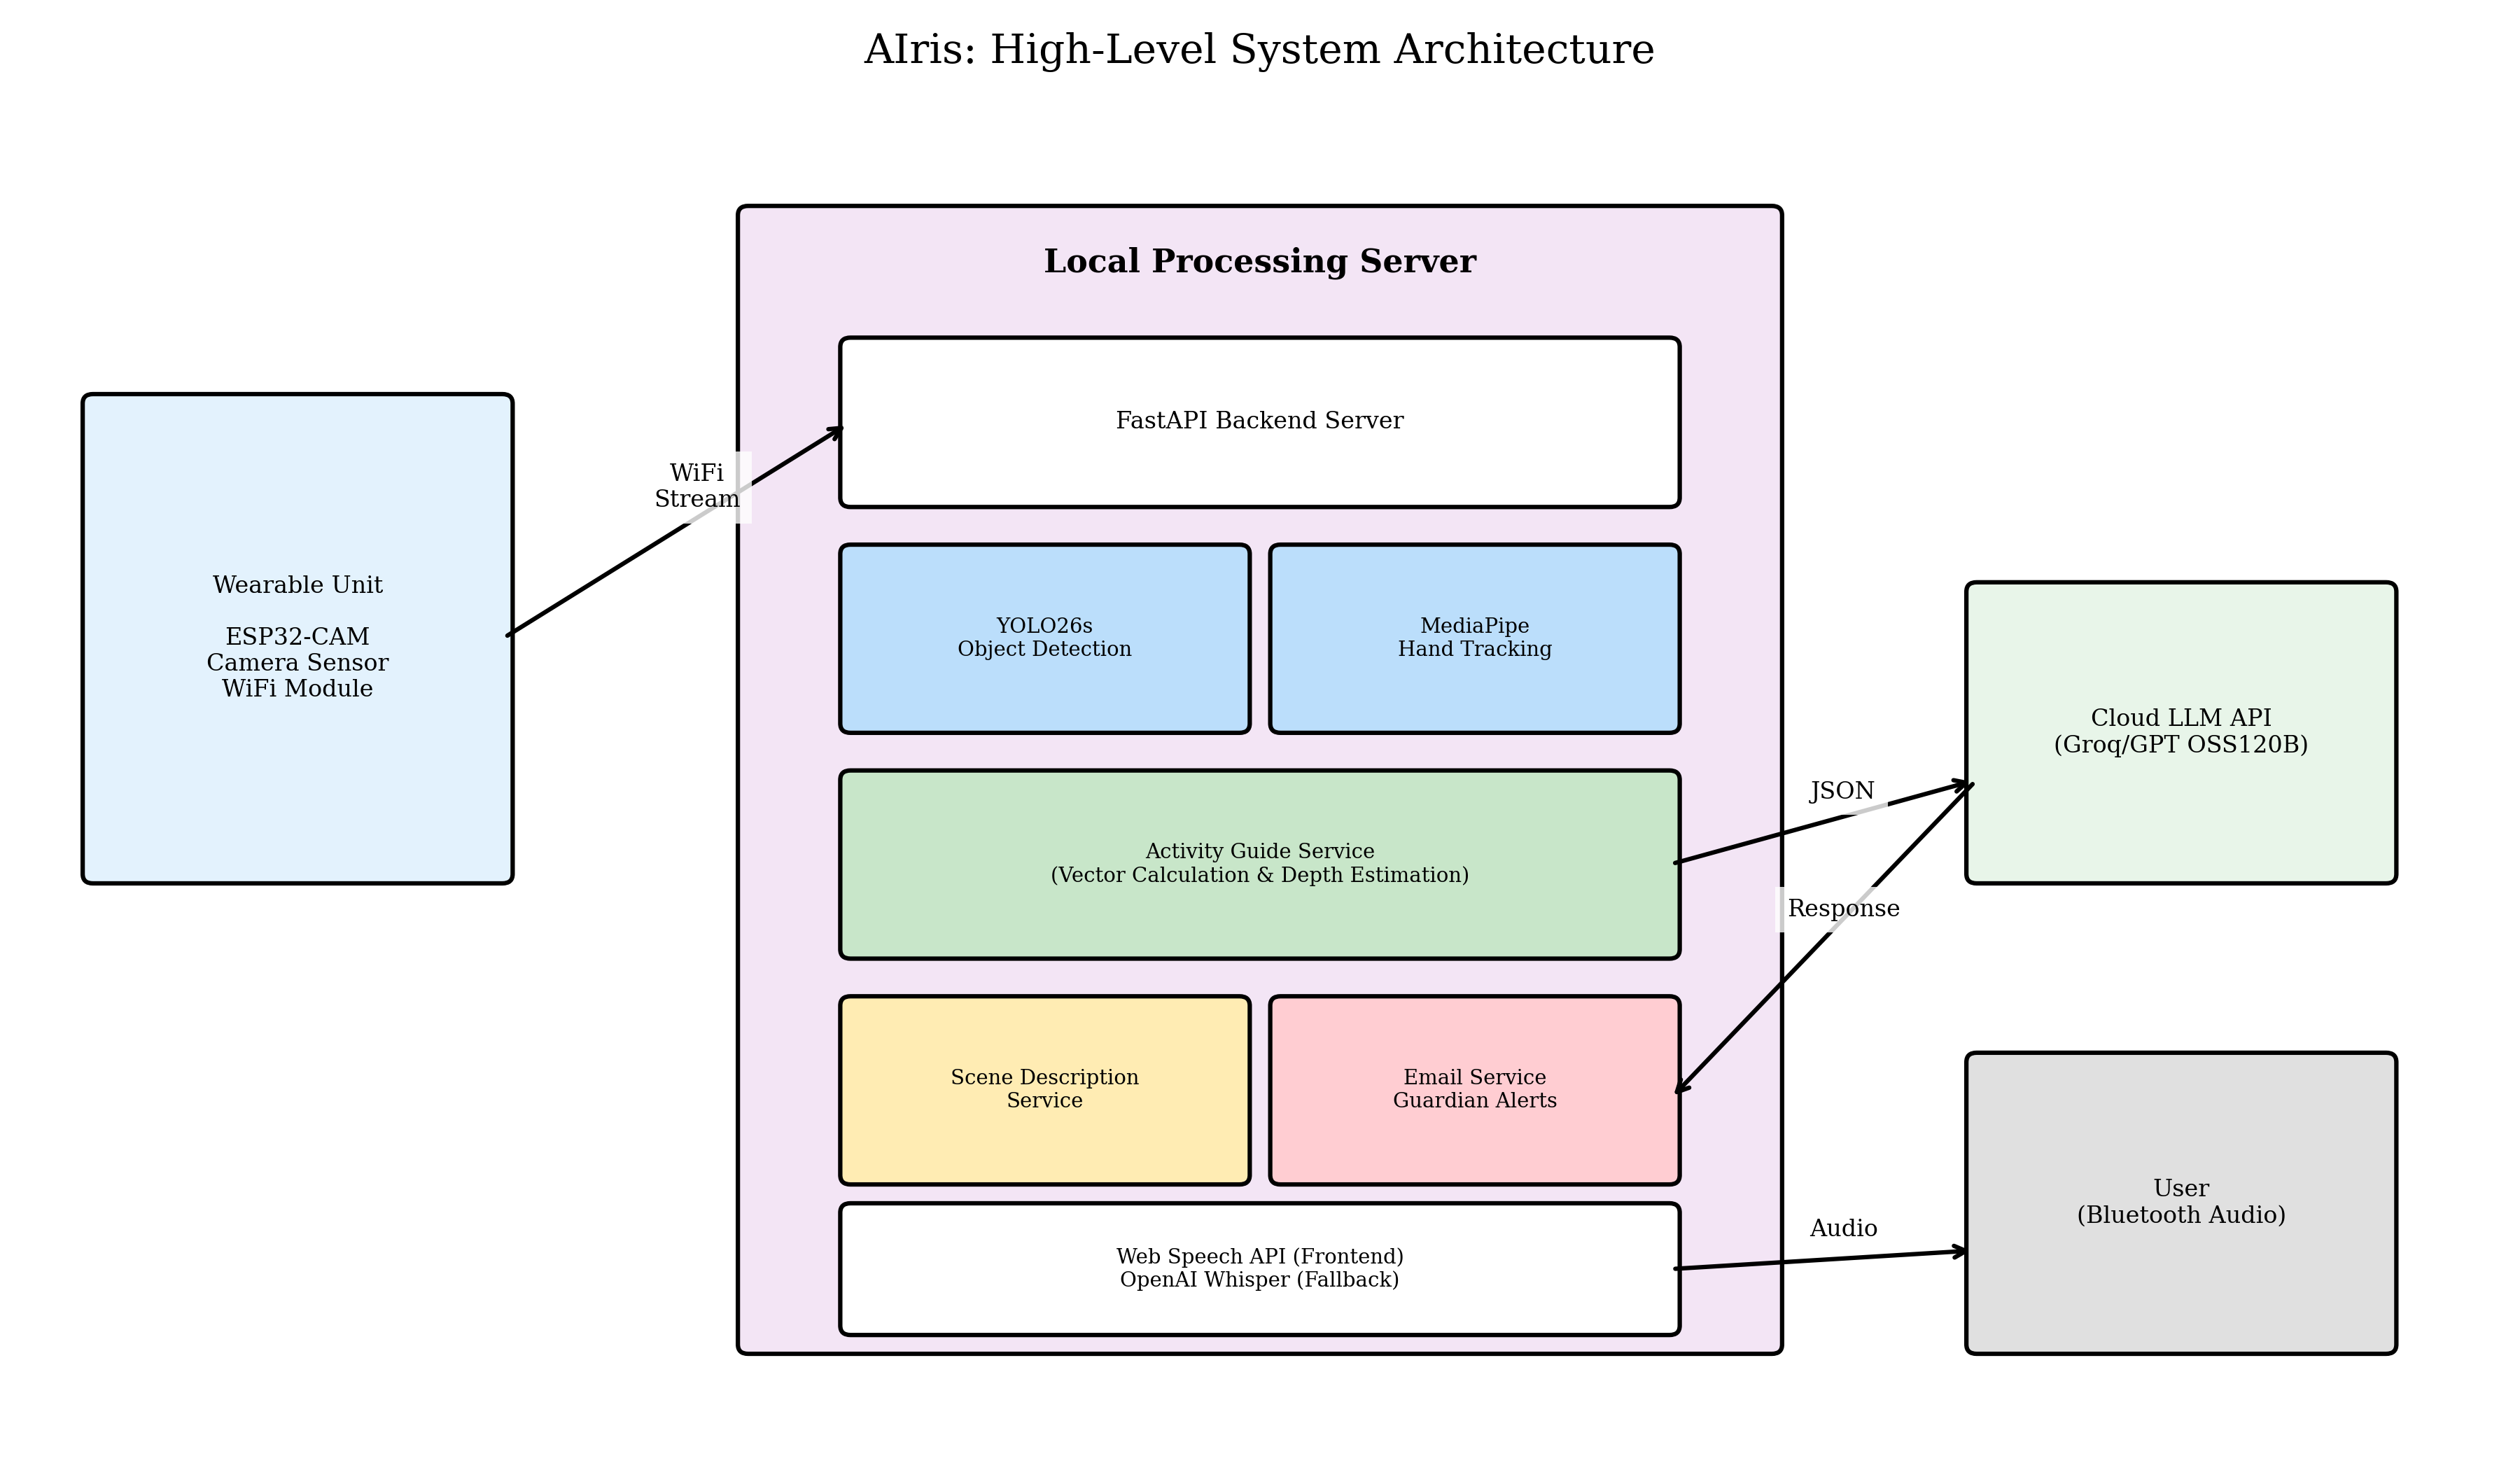
\includegraphics[width=1.0\textwidth]{diagrams/system_architecture.png}
\caption{High-level system architecture of AIris showing the separation between the wearable perception unit, local processing server, and cloud API services.}
\label{fig:architecture}
\end{figure}

\section{Hardware Subsystems}

\subsection{Wearable Perception Unit}

The visual perception unit of AIris is built around the ESP32-CAM development board, selected for its exceptional price-to-capability ratio. At a retail cost of approximately eight to ten dollars, the ESP32-CAM integrates a capable microcontroller unit, a two-megapixel OV2640 camera sensor, and complete WiFi connectivity in a compact form factor suitable for wearable integration. The ESP32-CAM module operates as a dedicated video streaming device in the AIris system. The firmware implements an HTTP-based interface with a stream endpoint that delivers MJPEG video encoded as a multipart HTTP response, enabling continuous frame transmission to the backend server over a local WiFi network.

\begin{table}[H]
\centering
\caption{Hardware Specification of the Wearable Perception Unit (ESP32-CAM)}
\label{tab:hardware_specs}
\begin{tabular}{@{}ll@{}}
\toprule
\textbf{Component} & \textbf{Specification} \\ \midrule
Microcontroller & ESP32-S SoC (Xtensa Dual-Core 32-bit LX6) \\
Clock Speed & Up to 240 MHz \\
Memory & 520 KB Internal SRAM + 4 MB External PSRAM \\
Camera Sensor & OV2640 (2 Megapixel) \\
Connectivity & WiFi 802.11 b/g/n + Bluetooth 4.2 / BLE \\
Power Consumption & approx. 180mA with flash off \\
Dimensions & 27 x 40.5 x 4.5 mm \\ \bottomrule
\end{tabular}
\end{table}

\subsection{Local Processing Server}

The computational core of AIris executes on a local server, which in typical deployment scenarios would be the user's laptop or a dedicated single-board computer. This server hosts all AI model inference including YOLO26s object detection, MediaPipe hand tracking, and BLIP image captioning. The design decision to perform processing locally rather than in the cloud addresses both the latency and privacy constraints identified in the problem statement. Local inference eliminates the network round-trip time inherent in cloud-based solutions and ensures that video data remains within the user's local network. The system has been optimized for Apple Silicon processors, with automatic detection and utilization of Metal Performance Shaders for GPU acceleration when available.

\subsection{Audio Interface}

The user interaction layer of AIris is entirely audio-based, reflecting the accessibility requirements of visually impaired users. The primary audio interface utilizes the Web Speech API, a browser-native capability that provides both speech recognition and speech synthesis without requiring additional dependencies or cloud API keys. This approach offers several advantages: zero-cost operation since all speech processing occurs natively in the browser, reduced latency compared to cloud-based alternatives, and improved privacy since voice data is processed locally. For backend fallback scenarios, the system also includes integration with OpenAI Whisper for speech-to-text and Google Text-to-Speech for audio generation.

\subsection{WiFi Network Connectivity}

The AIris system requires both the ESP32-CAM module and the local processing server to be connected to the same WiFi network for video streaming to function. This architectural requirement ensures low-latency communication while maintaining the privacy benefits of local processing, as all video data remains within the user's home network and never traverses the public internet.

\begin{figure}[H]
\centering
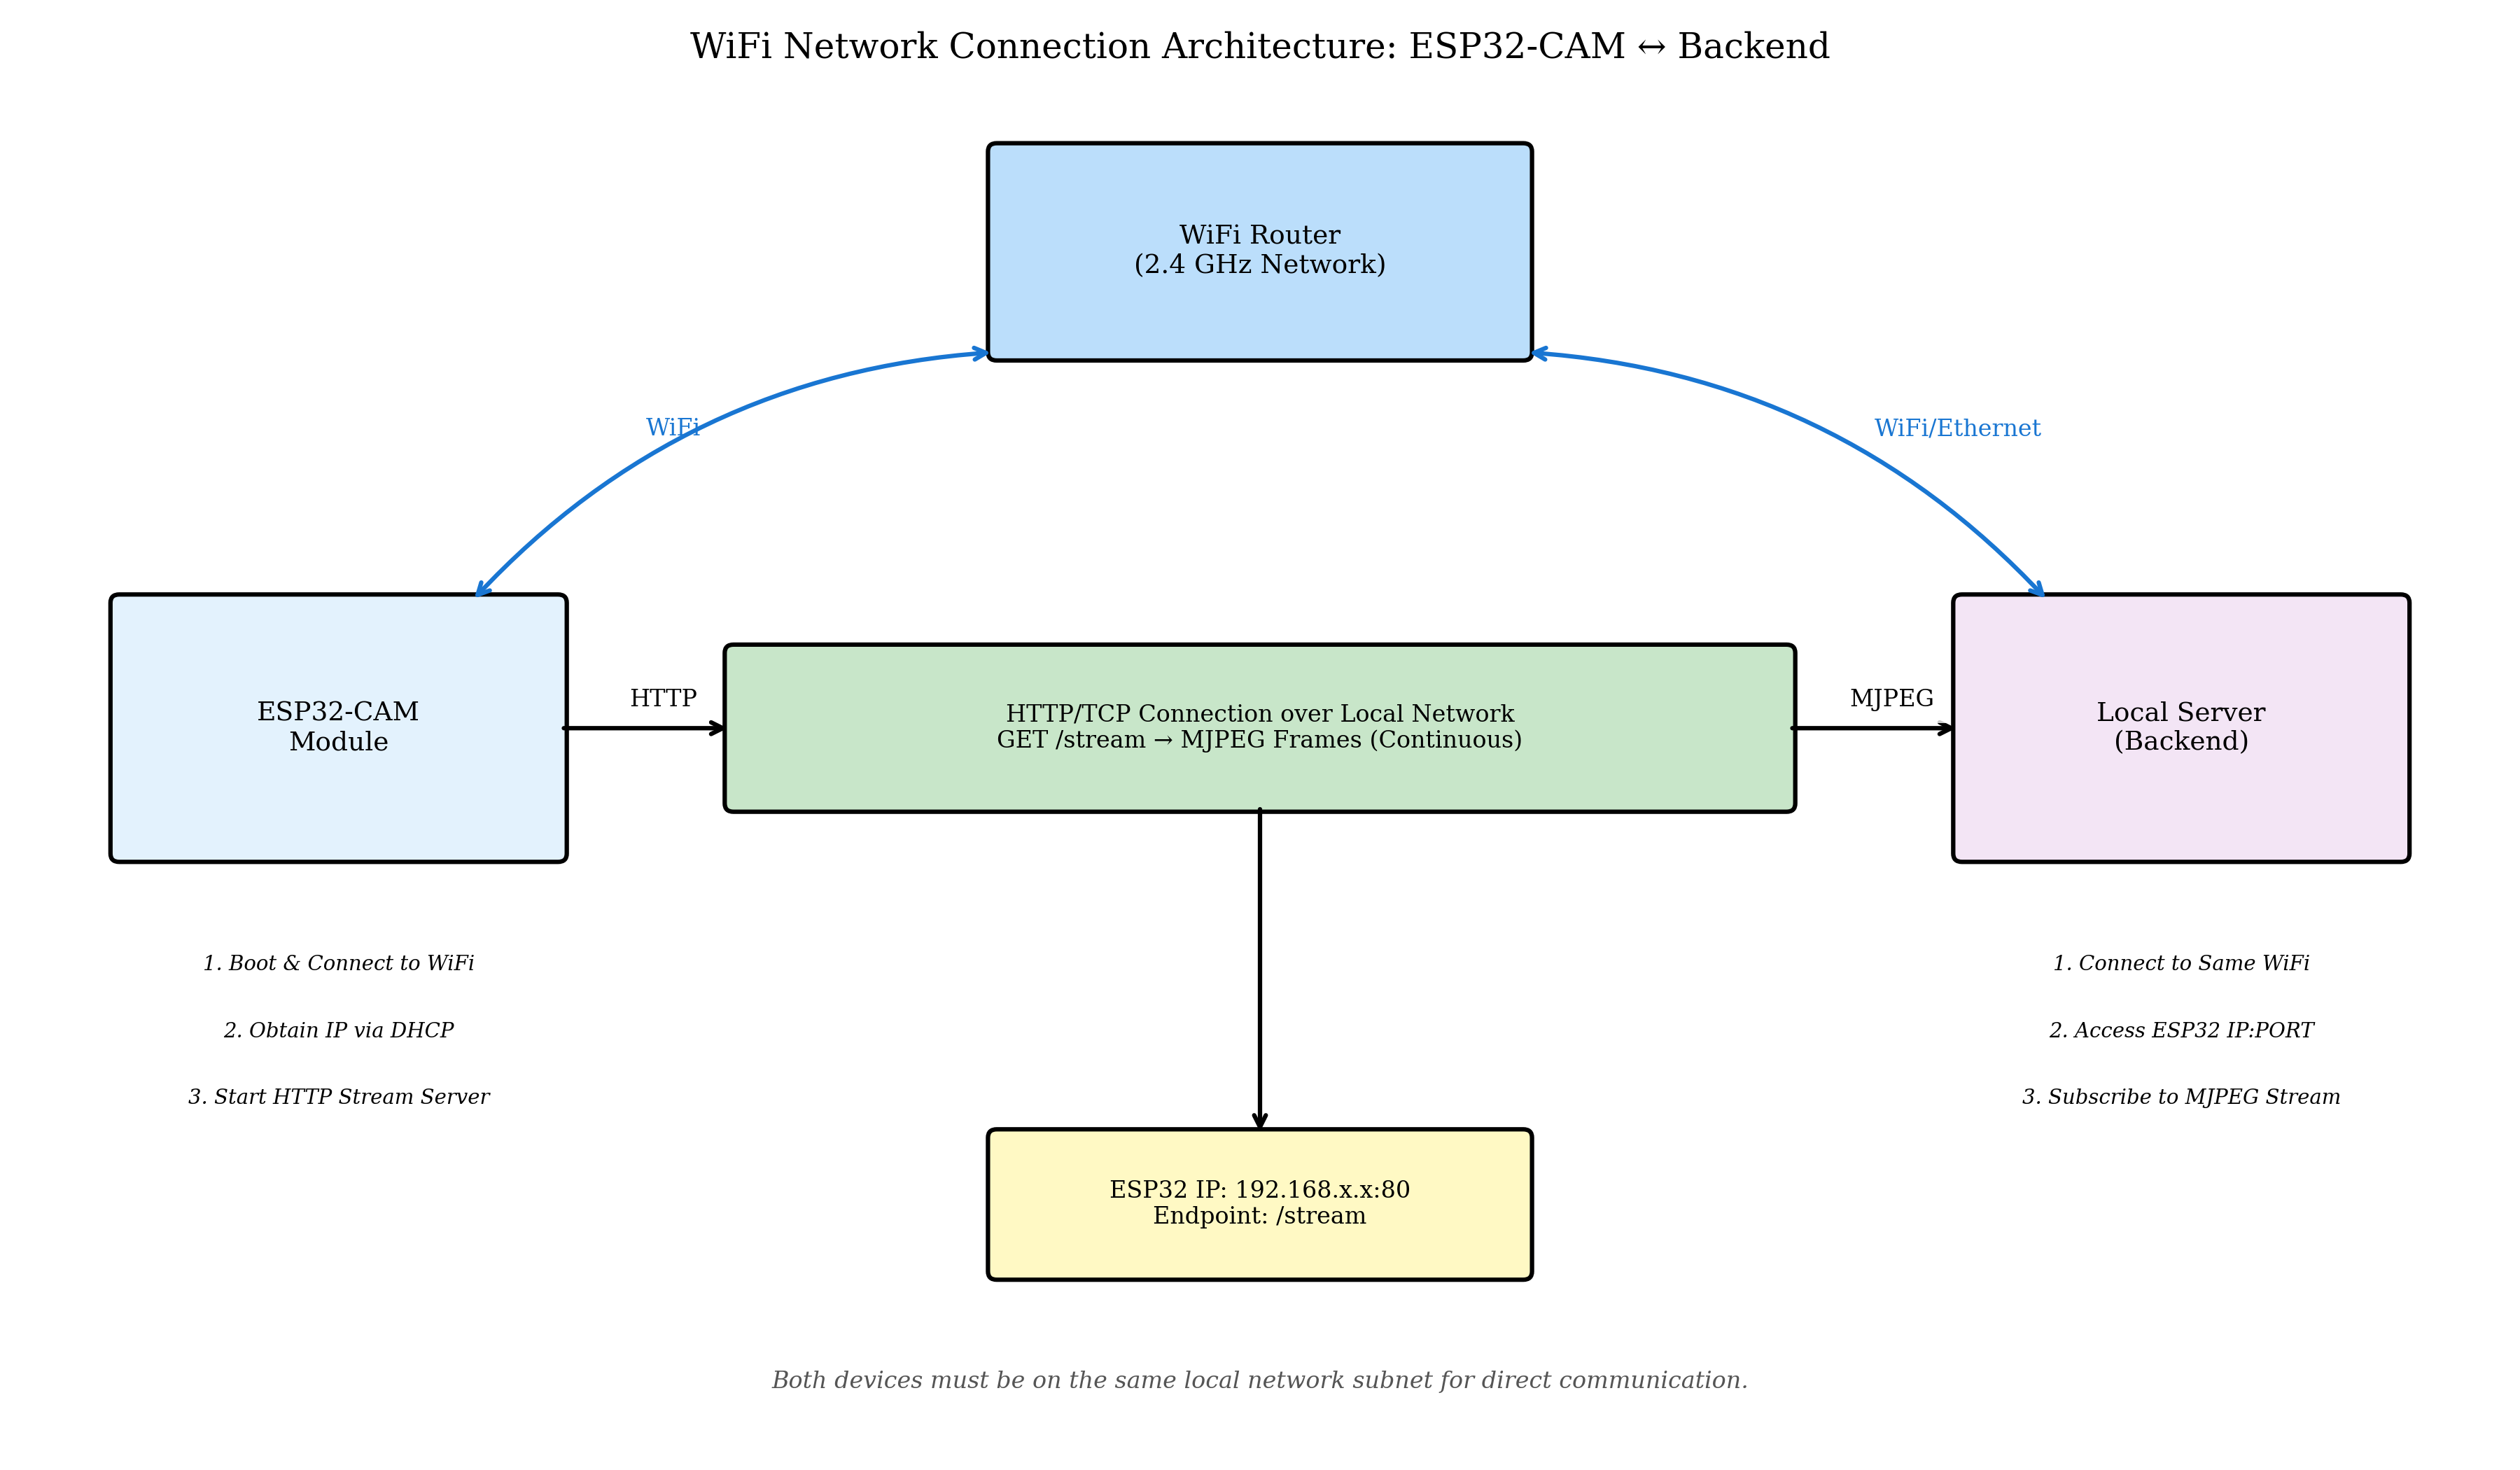
\includegraphics[width=1.0\textwidth]{diagrams/wifi_connection_flow.png}
\caption{WiFi network connection architecture showing how the ESP32-CAM and backend server establish communication through a shared local network.}
\label{fig:wifi_connection}
\end{figure}

The connection process begins when the ESP32-CAM module powers on and executes its firmware initialization routine. Rather than using hardcoded credentials, the firmware implements a flexible provisioning system using the ESP32's non-volatile storage (NVS) through the Preferences library. On first boot or after a credential reset, the device enters Access Point mode, broadcasting an open network named ``ESP32-CAM-SETUP'' that allows users to configure the target WiFi network through a simple HTTP interface. Once credentials are stored, subsequent boots attempt to connect to the configured network, typically operating on the 2.4 GHz band which offers superior range and wall penetration compared to 5 GHz alternatives. Upon successful association with the access point, the ESP32-CAM obtains an IP address through the Dynamic Host Configuration Protocol (DHCP), after which it initializes an HTTP server on port 80 that exposes multiple endpoints including the MJPEG video stream at the \texttt{/stream} path.

The local processing server, which may be the user's laptop or a dedicated single-board computer, connects to the same WiFi network either wirelessly or through a wired Ethernet connection to the router. The backend application requires knowledge of the ESP32-CAM's IP address to establish the video stream connection. The ESP32-CAM firmware outputs its assigned IP address to the serial port in a parseable format, and also exposes a \texttt{/ip} endpoint for programmatic discovery. In the current implementation, this IP address is configured manually through the frontend interface, though future iterations may implement automatic device discovery through mDNS or similar zero-configuration networking protocols.

Once both devices are connected to the same network subnet, the backend's Camera Service initiates an HTTP GET request to the ESP32-CAM's \texttt{/stream} endpoint. The ESP32-CAM responds with a multipart MIME response of type \texttt{multipart/x-mixed-replace} containing continuous JPEG frames, which the Camera Service decodes and buffers for downstream processing. This streaming architecture enables real-time video transmission with typical latencies of 30 to 50 milliseconds for the network transport component alone. The requirement for same-network connectivity represents a deliberate design tradeoff that prioritizes privacy and latency over the flexibility of cloud-based architectures.

\section{Software Architecture}

The software architecture follows a service-oriented design implemented using the FastAPI web framework for Python. This design enables modular development and testing of individual system components while providing the high-performance asynchronous request handling necessary for real-time video processing.

\subsection{Backend Service Organization}

The backend comprises several specialized services that collectively implement the AIris functionality. The Camera Service manages connections to video sources, whether the ESP32-CAM streaming endpoint or a local webcam for testing purposes. This service abstracts the video source details from downstream processing, enabling seamless switching between camera sources without modifying the rest of the pipeline. It implements a frame buffer mechanism for ESP32 sources to smooth out network-induced frame rate variations.

The Model Service handles the loading and inference of all AI models. It implements intelligent device detection that automatically selects the optimal computing backend, preferring Metal Performance Shaders on Apple Silicon, CUDA on NVIDIA GPUs, and falling back to CPU otherwise. The service uses lazy loading strategies that defer model initialization until first use and cache model instances to avoid repeated loading overhead.

The Activity Guide Service implements the core Active Guidance functionality, maintaining the state machine that tracks the progress of object-finding tasks and generating directional instructions based on the relative positions of the detected target object and the user's hand. The Scene Description Service provides continuous environmental awareness by periodically analyzing video frames and synthesizing descriptions through LLM reasoning.

The Email Service manages communication with designated guardians through Gmail SMTP, implementing sophisticated logic for alert triggering, configurable risk thresholds, cooldown periods to prevent notification fatigue, and generation of daily and weekly activity summaries with branded HTML templates.


\chapter{The Activity Guidance Algorithm}

\section{Conceptual Foundation}

The Active Guidance feature represents the primary technical contribution of the AIris project, distinguishing it from existing assistive systems that provide only passive environmental descriptions. The fundamental insight underlying Active Guidance is that knowing the location of an object is insufficient for enabling physical interaction; the user must be guided through the spatial trajectory from their current hand position to the target object.

\begin{figure}[H]
\centering
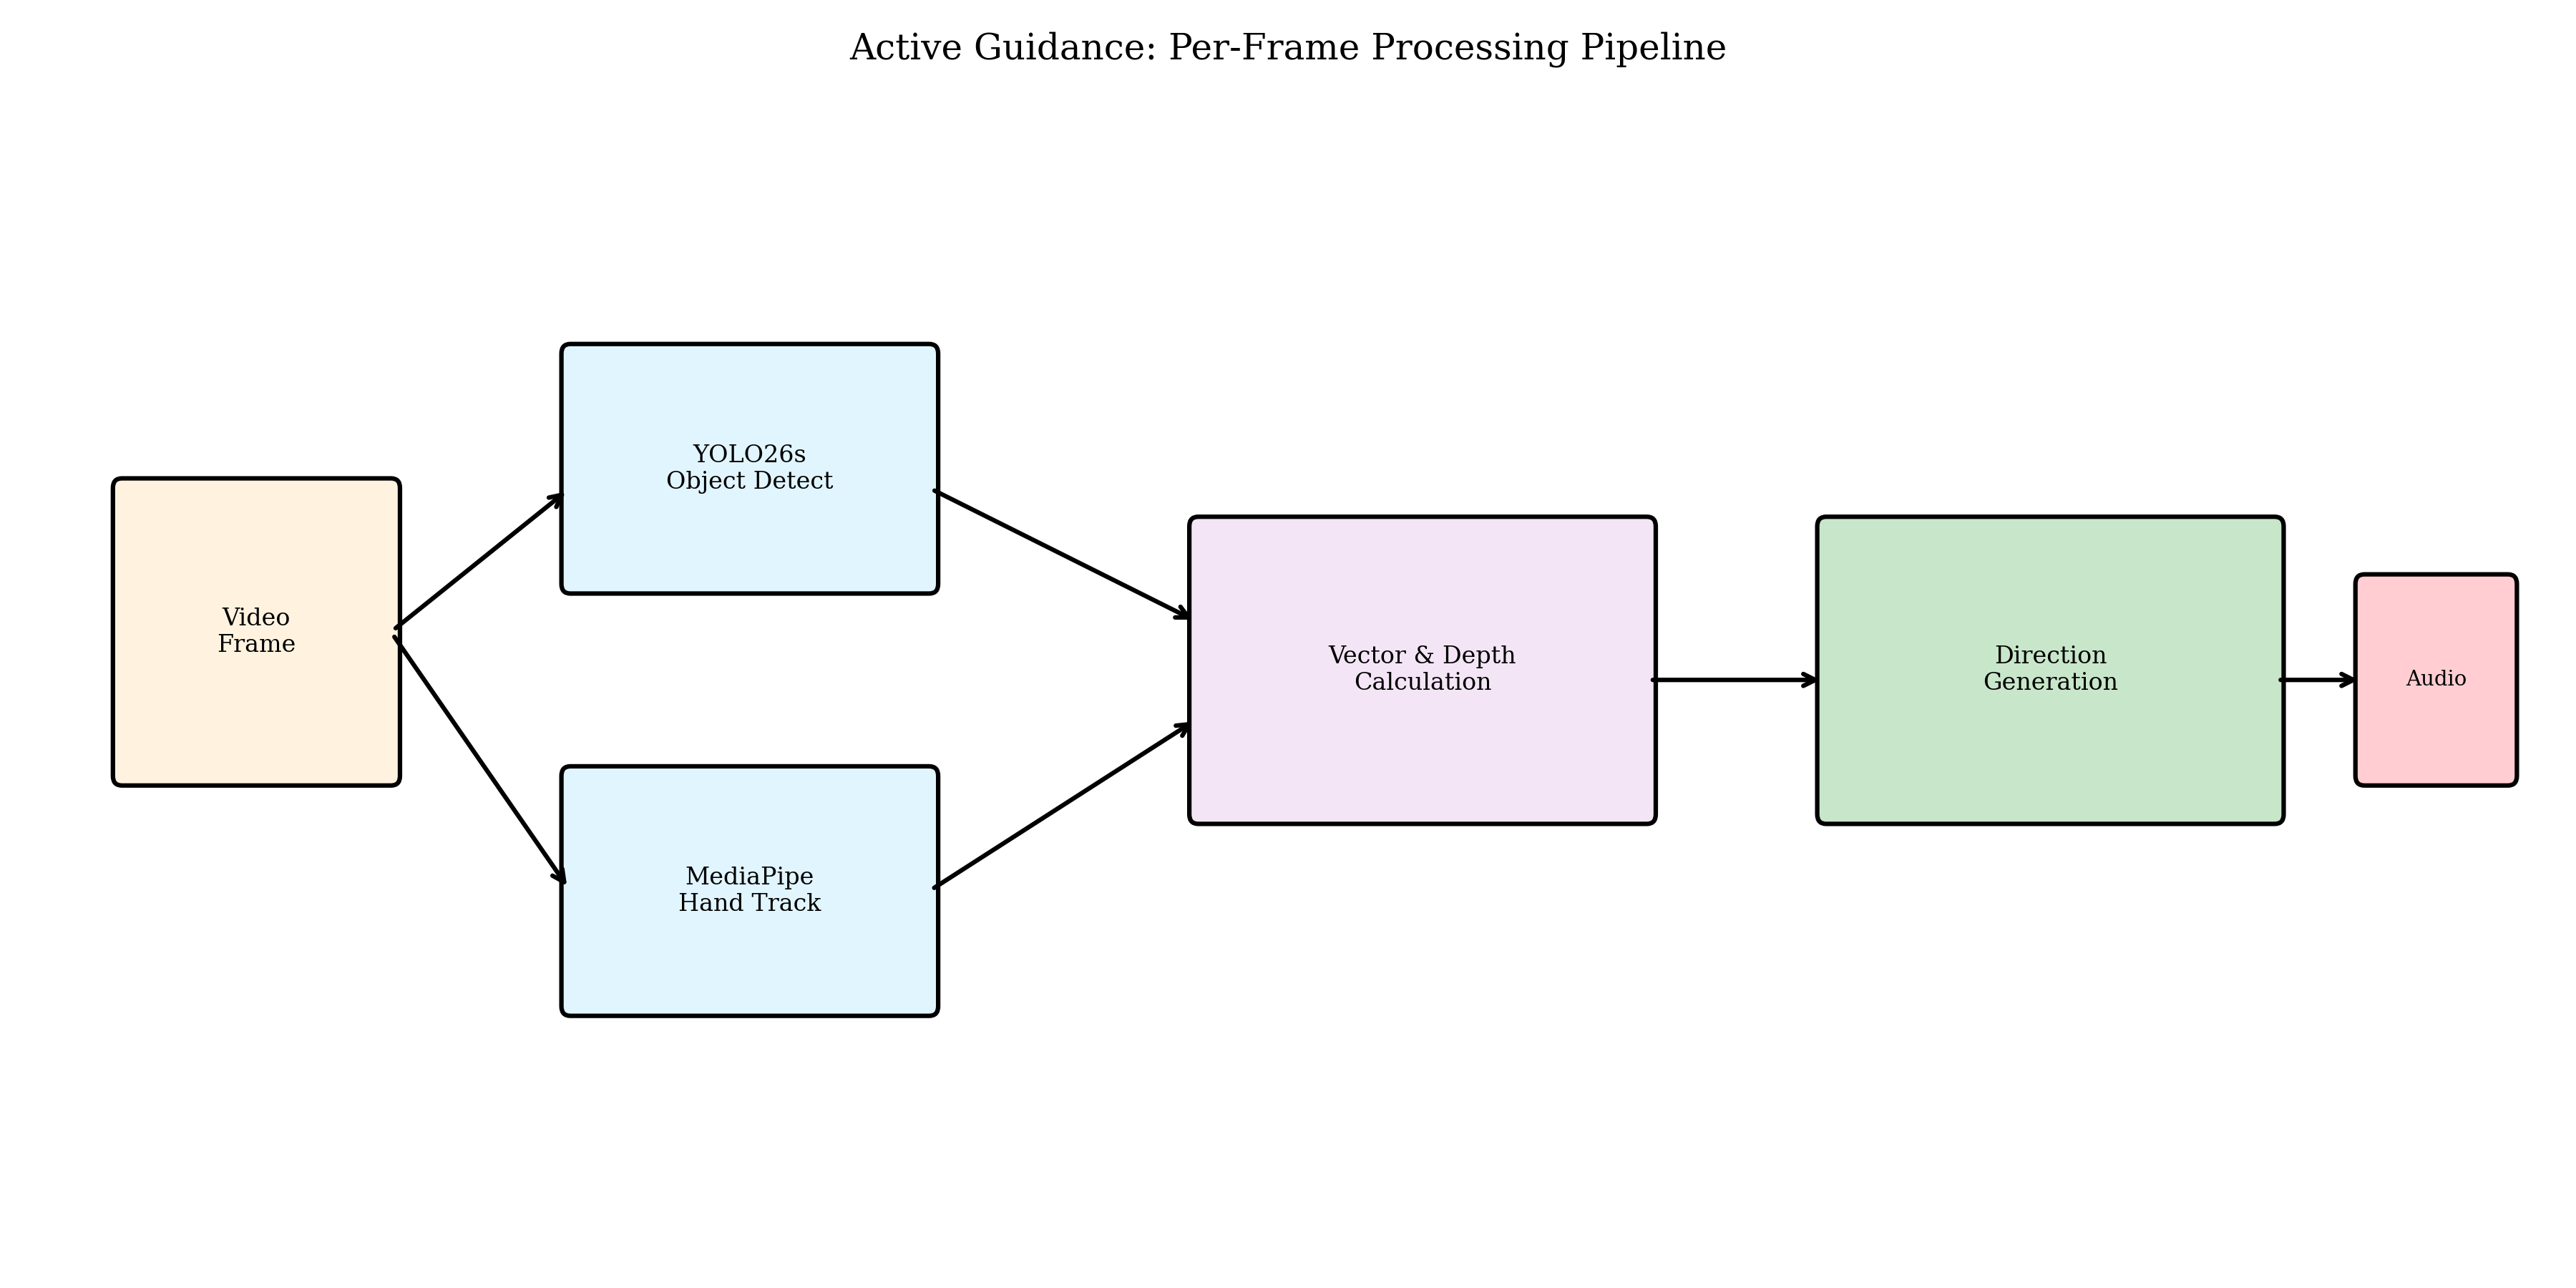
\includegraphics[width=1.0\textwidth]{diagrams/guidance_pipeline.png}
\caption{The per-frame processing pipeline for the Active Guidance System, showing the parallel execution of object detection and hand tracking followed by vector-based direction generation.}
\label{fig:guidance_pipeline}
\end{figure}

The Active Guidance system operates as a closed-loop controller in which the user's hand position and the target object location serve as the measured and reference signals, respectively. Each video frame triggers a cycle of perception, calculation, and instruction generation that progressively reduces the error between these signals until the hand successfully reaches the object.

\section{State Machine Design}

The lifecycle of an Active Guidance task is modeled as a finite state machine with well-defined states and transitions. This formalization ensures predictable system behavior and facilitates both implementation and debugging.

\begin{figure}[H]
\centering
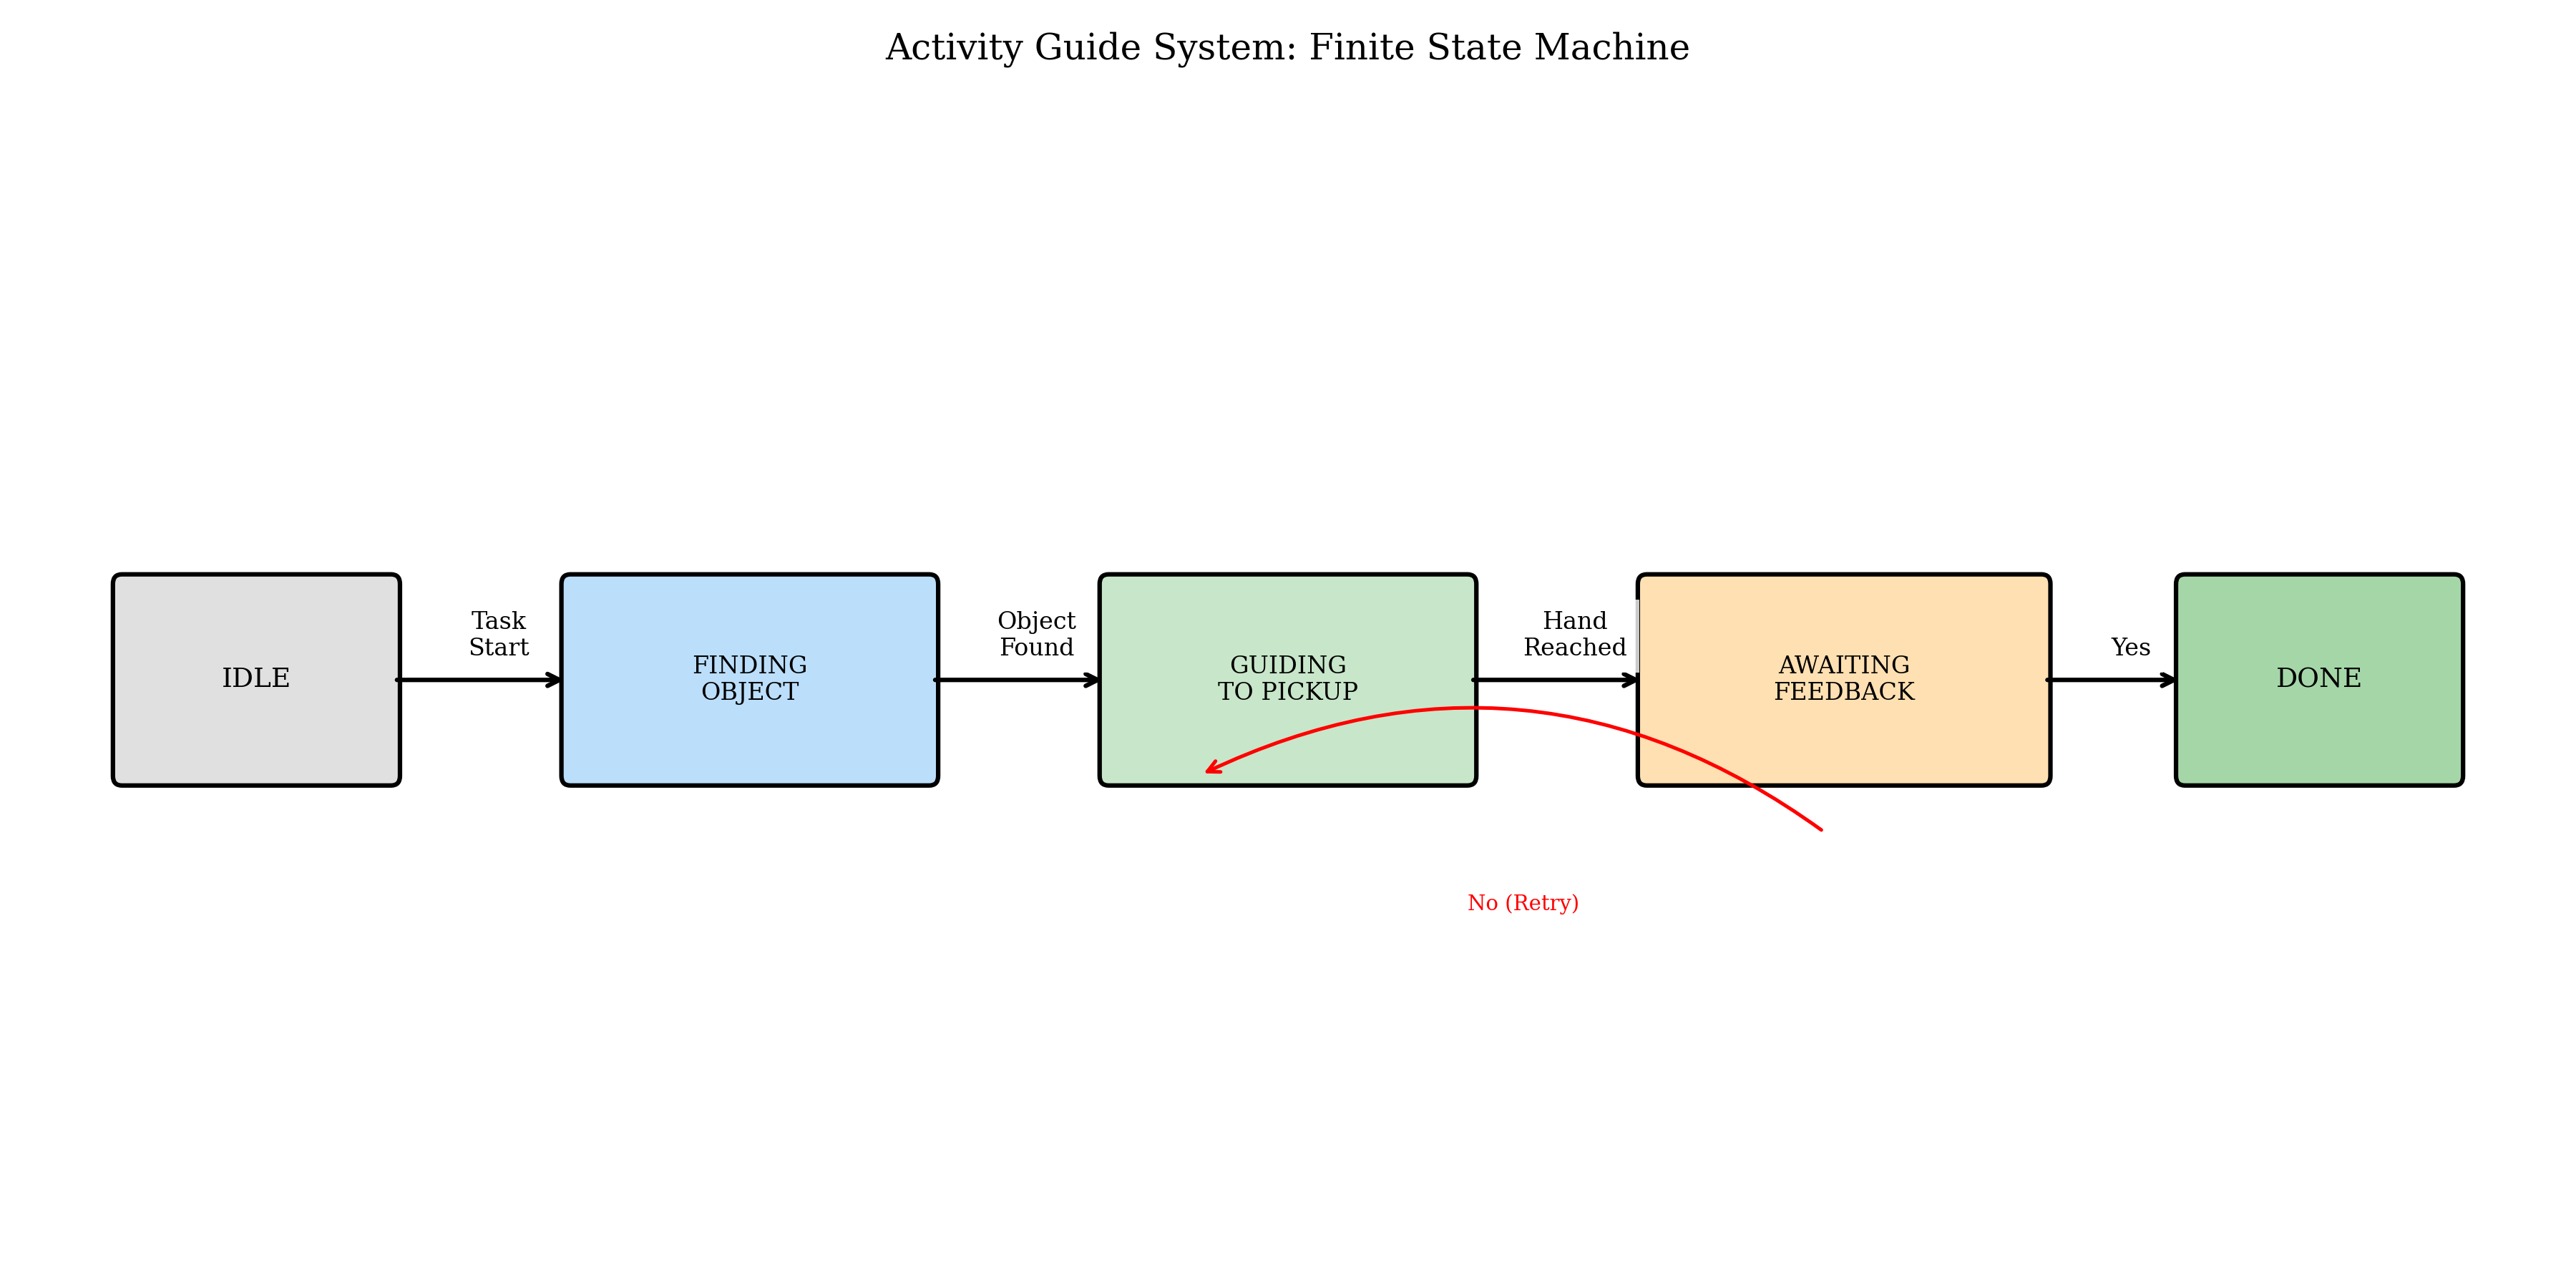
\includegraphics[width=0.95\textwidth]{diagrams/state_machine.png}
\caption{The finite state machine governing the Active Guidance task lifecycle, showing all states and transition conditions.}
\label{fig:state_machine}
\end{figure}

The IDLE state represents the initial condition when no task is active. Upon receiving a voice command from the user, the system transitions to FINDING\_OBJECT. In this state, the system actively searches for the target object in each incoming video frame using YOLO26s detection. Once the target object is detected with sufficient confidence, the system transitions to GUIDING\_TO\_PICKUP and begins providing directional instructions. When the system determines that the user's hand has reached the object based on proximity metrics, it transitions to AWAITING\_FEEDBACK and requests verbal confirmation from the user. A positive confirmation results in transition to the DONE state, while a negative response returns the system to FINDING\_OBJECT to locate an alternative instance of the target.

\section{Vector-Based Guidance Logic}

The core of the Active Guidance system is the algorithm that translates the spatial relationship between the hand and target object into natural language directional instructions. This translation must account for the geometric properties of the camera configuration, particularly the mirror effect inherent in front-facing cameras.

\begin{algorithm}[H]
\caption{Generate Directional Guidance}
\begin{algorithmic}[1]
\Require HandBox $B_h = (x_1^h, y_1^h, x_2^h, y_2^h)$, ObjectBox $B_o = (x_1^o, y_1^o, x_2^o, y_2^o)$, Frame dimensions $(W, H)$
\Ensure Direction string $D$

\State $C_h \gets \left(\frac{x_1^h + x_2^h}{2}, \frac{y_1^h + y_2^h}{2}\right)$ \Comment{Hand center}
\State $C_o \gets \left(\frac{x_1^o + x_2^o}{2}, \frac{y_1^o + y_2^o}{2}\right)$ \Comment{Object center}
\State $\Delta x \gets C_o^x - C_h^x$ \Comment{Horizontal displacement}
\State $\Delta y \gets C_o^y - C_h^y$ \Comment{Vertical displacement}

\State $A_h \gets (x_2^h - x_1^h) \times (y_2^h - y_1^h)$ \Comment{Hand area}
\State $A_o \gets (x_2^o - x_1^o) \times (y_2^o - y_1^o)$ \Comment{Object area}
\State $r_{depth} \gets A_o / A_h$ \Comment{Depth ratio}

\State $Directions \gets []$

\If{$r_{depth} < 0.4$} \Comment{Object closer to body}
    \State $Directions$.append("back towards you")
\ElsIf{$r_{depth} > 2.5$} \Comment{Object farther from body}
    \State $Directions$.append("forward away from you")
\EndIf

\If{$|\Delta x| > 0.05 \times W$} \Comment{Apply mirror correction}
    \If{$\Delta x > 0$}
        \State $Directions$.append("left") \Comment{Inverted for front-facing camera}
    \Else
        \State $Directions$.append("right")
    \EndIf
\EndIf

\If{$|\Delta y| > 0.05 \times H$}
    \If{$\Delta y > 0$}
        \State $Directions$.append("down")
    \Else
        \State $Directions$.append("up")
    \EndIf
\EndIf

\State \Return "Move your hand " + join($Directions$, ", ")
\end{algorithmic}
\end{algorithm}

\begin{table}[H]
\centering
\caption{Directional Guidance Vocabulary Mapping}
\label{tab:guidance_vocab}
\begin{tabular}{@{}lll@{}}
\toprule
\textbf{Condition} & \textbf{Threshold} & \textbf{Audio Instruction} \\ \midrule
Horizontal Offset ($|\Delta x|$) & $> 5\%$ of frame width & ``Move Left'' / ``Move Right'' \\
Vertical Offset ($|\Delta y|$) & $> 5\%$ of frame height & ``Move Up'' / ``Move Down'' \\
Depth Ratio ($r_{depth}$) & $< 0.4$ (Object small) & ``Back towards you'' \\
Depth Ratio ($r_{depth}$) & $> 2.5$ (Object large) & ``Forward away from you'' \\
Hand Reached & Proximity Check True & ``Object reached. Confirm?'' \\ \bottomrule
\end{tabular}
\end{table}

\section{Monocular Depth Estimation}

A significant challenge in the Active Guidance system is the inference of depth information from a single RGB camera, which inherently captures only a two-dimensional projection of the three-dimensional scene. Commercial depth cameras address this problem through active sensing technologies, but the cost and power constraints of the AIris wearable hardware preclude their use.

Our solution leverages a heuristic based on the relationship between object size in the image plane and its distance from the camera. Under the assumptions of perspective projection, the apparent size of an object decreases as its distance from the camera increases. By comparing the bounding box areas of the hand and the target object, we can infer their relative depths.

The depth ratio $r_{depth}$ is computed as the ratio of the object bounding box area to the hand bounding box area. A ratio significantly less than one indicates that the object appears smaller than the hand, suggesting that it is located closer to the user's body than the hand currently is. Conversely, a ratio significantly greater than one indicates that the object extends farther from the body. This heuristic provides directional guidance rather than metric distance measurements, which is sufficient for the qualitative instructions such as reach forward or move your hand back that constitute the depth component of Active Guidance feedback.

\section{Hand-Object Proximity Detection}

Determining when the user's hand has successfully reached the target object is a critical decision point that triggers the transition from active guidance to confirmation. This determination must balance sensitivity to avoid premature declarations of success with responsiveness to avoid frustrating the user with continued instructions after they have already grasped the object.

\begin{algorithm}[H]
\caption{Determine if Hand Has Reached Object}
\begin{algorithmic}[1]
\Require HandBox $B_h$, ObjectBox $B_o$, Frame dimensions $(W, H)$
\Ensure Boolean indicating whether hand has reached object

\State $distance \gets \|C_o - C_h\|_2$ \Comment{Euclidean distance between centers}
\State $iou \gets \textsc{ComputeIoU}(B_h, B_o)$ \Comment{Intersection over Union}
\State $overlap \gets \textsc{ComputeOverlapRatio}(B_h, B_o)$ \Comment{Overlap area / Object area}

\State $r_{depth} \gets A_o / A_h$ \Comment{Depth ratio as before}
\State $depth\_similar \gets (0.3 \leq r_{depth} \leq 3.0)$

\State $proximity\_2d \gets (distance < 100) \textbf{ OR } (iou > 0.3) \textbf{ OR } (overlap > 0.4)$

\State \Return $proximity\_2d$ \textbf{ AND } $depth\_similar$
\end{algorithmic}
\end{algorithm}

The algorithm combines multiple geometric metrics to achieve robust detection. The center distance provides a basic proximity measure in pixel units. The Intersection over Union metric captures the overlap between the hand and object bounding boxes normalized by their union area. The overlap ratio specifically addresses scenarios where the hand partially occludes the object. The conjunction of two-dimensional proximity with depth similarity ensures that the system does not prematurely declare success when the hand passes in front of or behind the object without actually reaching it.


\chapter{Scene Description and Safety Monitoring}

\section{Continuous Environmental Awareness}

While Active Guidance addresses the problem of targeted object interaction, daily life also requires general awareness of the surrounding environment. The Scene Description mode of AIris provides this situational awareness through continuous frame analysis and periodic audio summaries.

The Scene Description service operates at a lower temporal resolution than Active Guidance, analyzing approximately two frames per second rather than every captured frame. This reduced rate reflects the less time-critical nature of scene understanding compared to real-time guidance and enables more computationally expensive analysis including LLM reasoning. The service maintains a buffer of five consecutive BLIP-generated frame descriptions, which are then submitted to the LLM for synthesis into a coherent narrative summary that captures the temporal evolution of the scene.

\section{The Fall Detection System}

Falls represent a significant health risk for visually impaired individuals, who are inherently more susceptible to tripping hazards and collision accidents. Prompt detection of falls and notification of caregivers can dramatically reduce the severity of outcomes by ensuring timely assistance.

\begin{figure}[H]
\centering
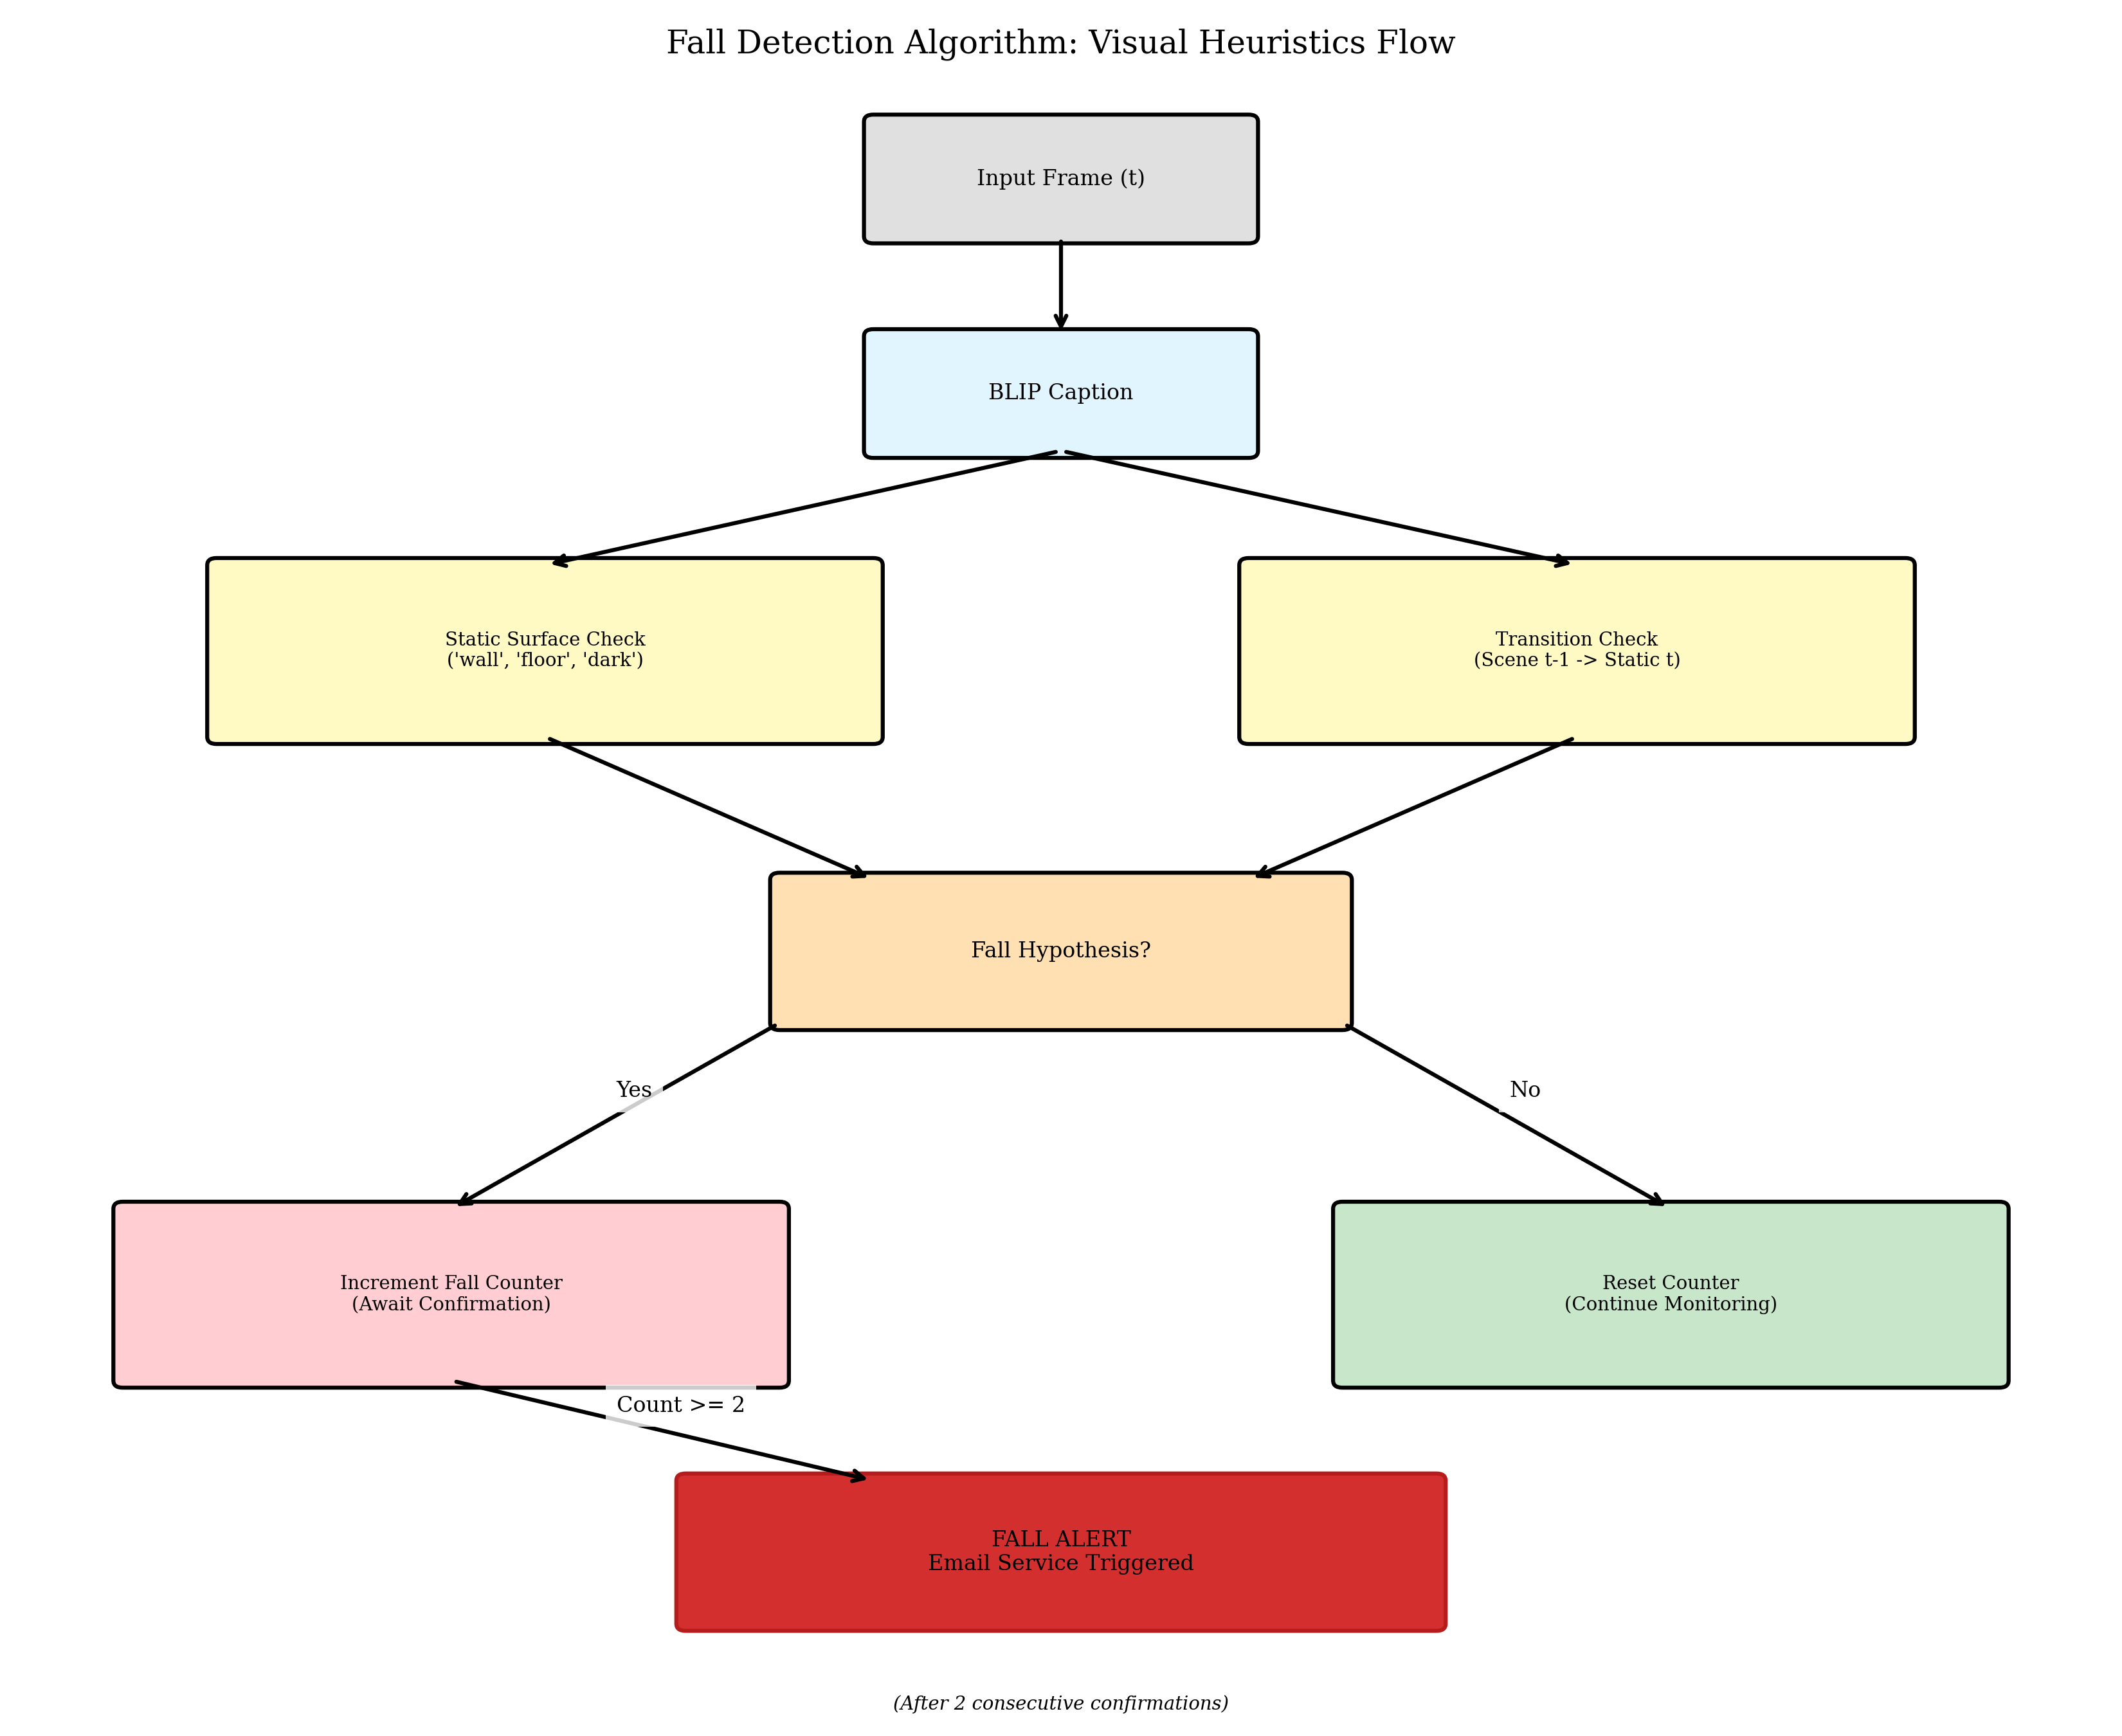
\includegraphics[width=0.9\textwidth]{diagrams/fall_detection_flow.png}
\caption{The Fall Detection algorithm flow, showing the dual-path analysis through static surface detection and scene transition detection.}
\label{fig:fall_detection}
\end{figure}

The AIris Fall Detection system employs a novel vision-based approach that detects falls without requiring accelerometers or other motion sensors. The key insight is that a fall typically results in a characteristic visual signature: a sudden transition from a complex scene containing furniture, people, and objects to a static, uniform surface such as a floor, wall, or ceiling as the camera comes to rest facing an uninteresting direction.

\begin{algorithm}[H]
\caption{Visual Fall Detection Heuristic}
\begin{algorithmic}[1]
\Require Current frame description $D_t$, Previous frame description $D_{t-1}$
\Ensure Boolean indicating fall hypothesis

\State $StaticKeywords \gets \{\text{"wall"}, \text{"floor"}, \text{"ceiling"}, \text{"dark"}, \text{"blur"}\}$
\State $SceneKeywords \gets \{\text{"person"}, \text{"furniture"}, \text{"room"}, \text{"window"}, \text{"table"}\}$

\State $CurrIsStatic \gets \exists k \in StaticKeywords : k \in D_t$
\State $PrevHadScene \gets \exists k \in SceneKeywords : k \in D_{t-1}$

\If{$PrevHadScene$ \textbf{AND} $CurrIsStatic$}
    \State \Return \textbf{True} \Comment{Scene-to-static transition detected}
\EndIf

\State $ImmediateTriggers \gets \{\text{"darkness"}, \text{"skateboard"}, \text{"blur"}\}$
\If{$\exists k \in ImmediateTriggers : k \in D_t$}
    \State \Return \textbf{True} \Comment{Immediate danger indicator}
\EndIf

\State \Return \textbf{False}
\end{algorithmic}
\end{algorithm}

\begin{table}[H]
\centering
\caption{Fall Detection Heuristic Criteria}
\label{tab:fall_heuristics}
\begin{tabular}{@{}ll@{}}
\toprule
\textbf{Heuristic Type} & \textbf{Trigger Conditions} \\ \midrule
Static Surface Detection & Frame is dominated by ``floor'', ``wall'', or ``ceiling'' \\
Darkness Check & Frame is described as ``dark'', ``black'', or ``unclear'' \\
Transition Analysis & Scene $t-1$ was dynamic $\to$ Scene $t$ is static \\
Keyword Trigger & BLIP detects ``fall'', ``crash'', or ``lying down'' \\
Confirmation Hysteresis & Condition must persist for $\geq 2$ consecutive frames \\ \bottomrule
\end{tabular}
\end{table}

The algorithm employs a confirmation mechanism to reduce false positives. A single frame exhibiting fall-like characteristics does not immediately trigger an alert; rather, the system requires two consecutive frames meeting the fall criteria before dispatching a notification. This hysteresis prevents spurious alerts from momentary camera obstructions or rapid user movements.

\section{Guardian Notification System}

The Email Service implements the communication layer that connects the AIris safety monitoring to external caregivers. When a fall or other high-risk situation is detected, the service dispatches an immediate alert email containing the timestamp and any available contextual information. The email templates employ the AIris brand design language with high-contrast styling for maximum readability, featuring the brand gold color scheme and clear visual hierarchy.

To prevent notification fatigue, the system implements a configurable cooldown period between consecutive alerts. The default cooldown of five minutes ensures that multiple detections of the same ongoing situation do not generate a cascade of emails. Falls, however, are treated as critical events that bypass the cooldown mechanism to ensure immediate notification regardless of prior alert history. The risk threshold for triggering alerts is configurable between 0.1 and 0.5, with a default of 0.3, allowing users and caregivers to adjust sensitivity based on individual needs.

Beyond immediate alerts, the Email Service generates periodic summary reports that provide caregivers with an overview of the user's activity patterns. Daily summaries include total event counts, location tracking based on scene descriptions, and highlighted safety incidents. Weekly summaries aggregate this information across seven days and identify trends in activity levels or risk exposure.


\chapter{Technical Implementation}

\section{System Sequence Flow}

The complete interaction sequence from user command to task completion involves coordination among all AIris subsystems. Understanding this flow is essential for appreciating how the conceptual algorithms described in previous chapters translate to practical operation.

\begin{figure}[H]
\centering
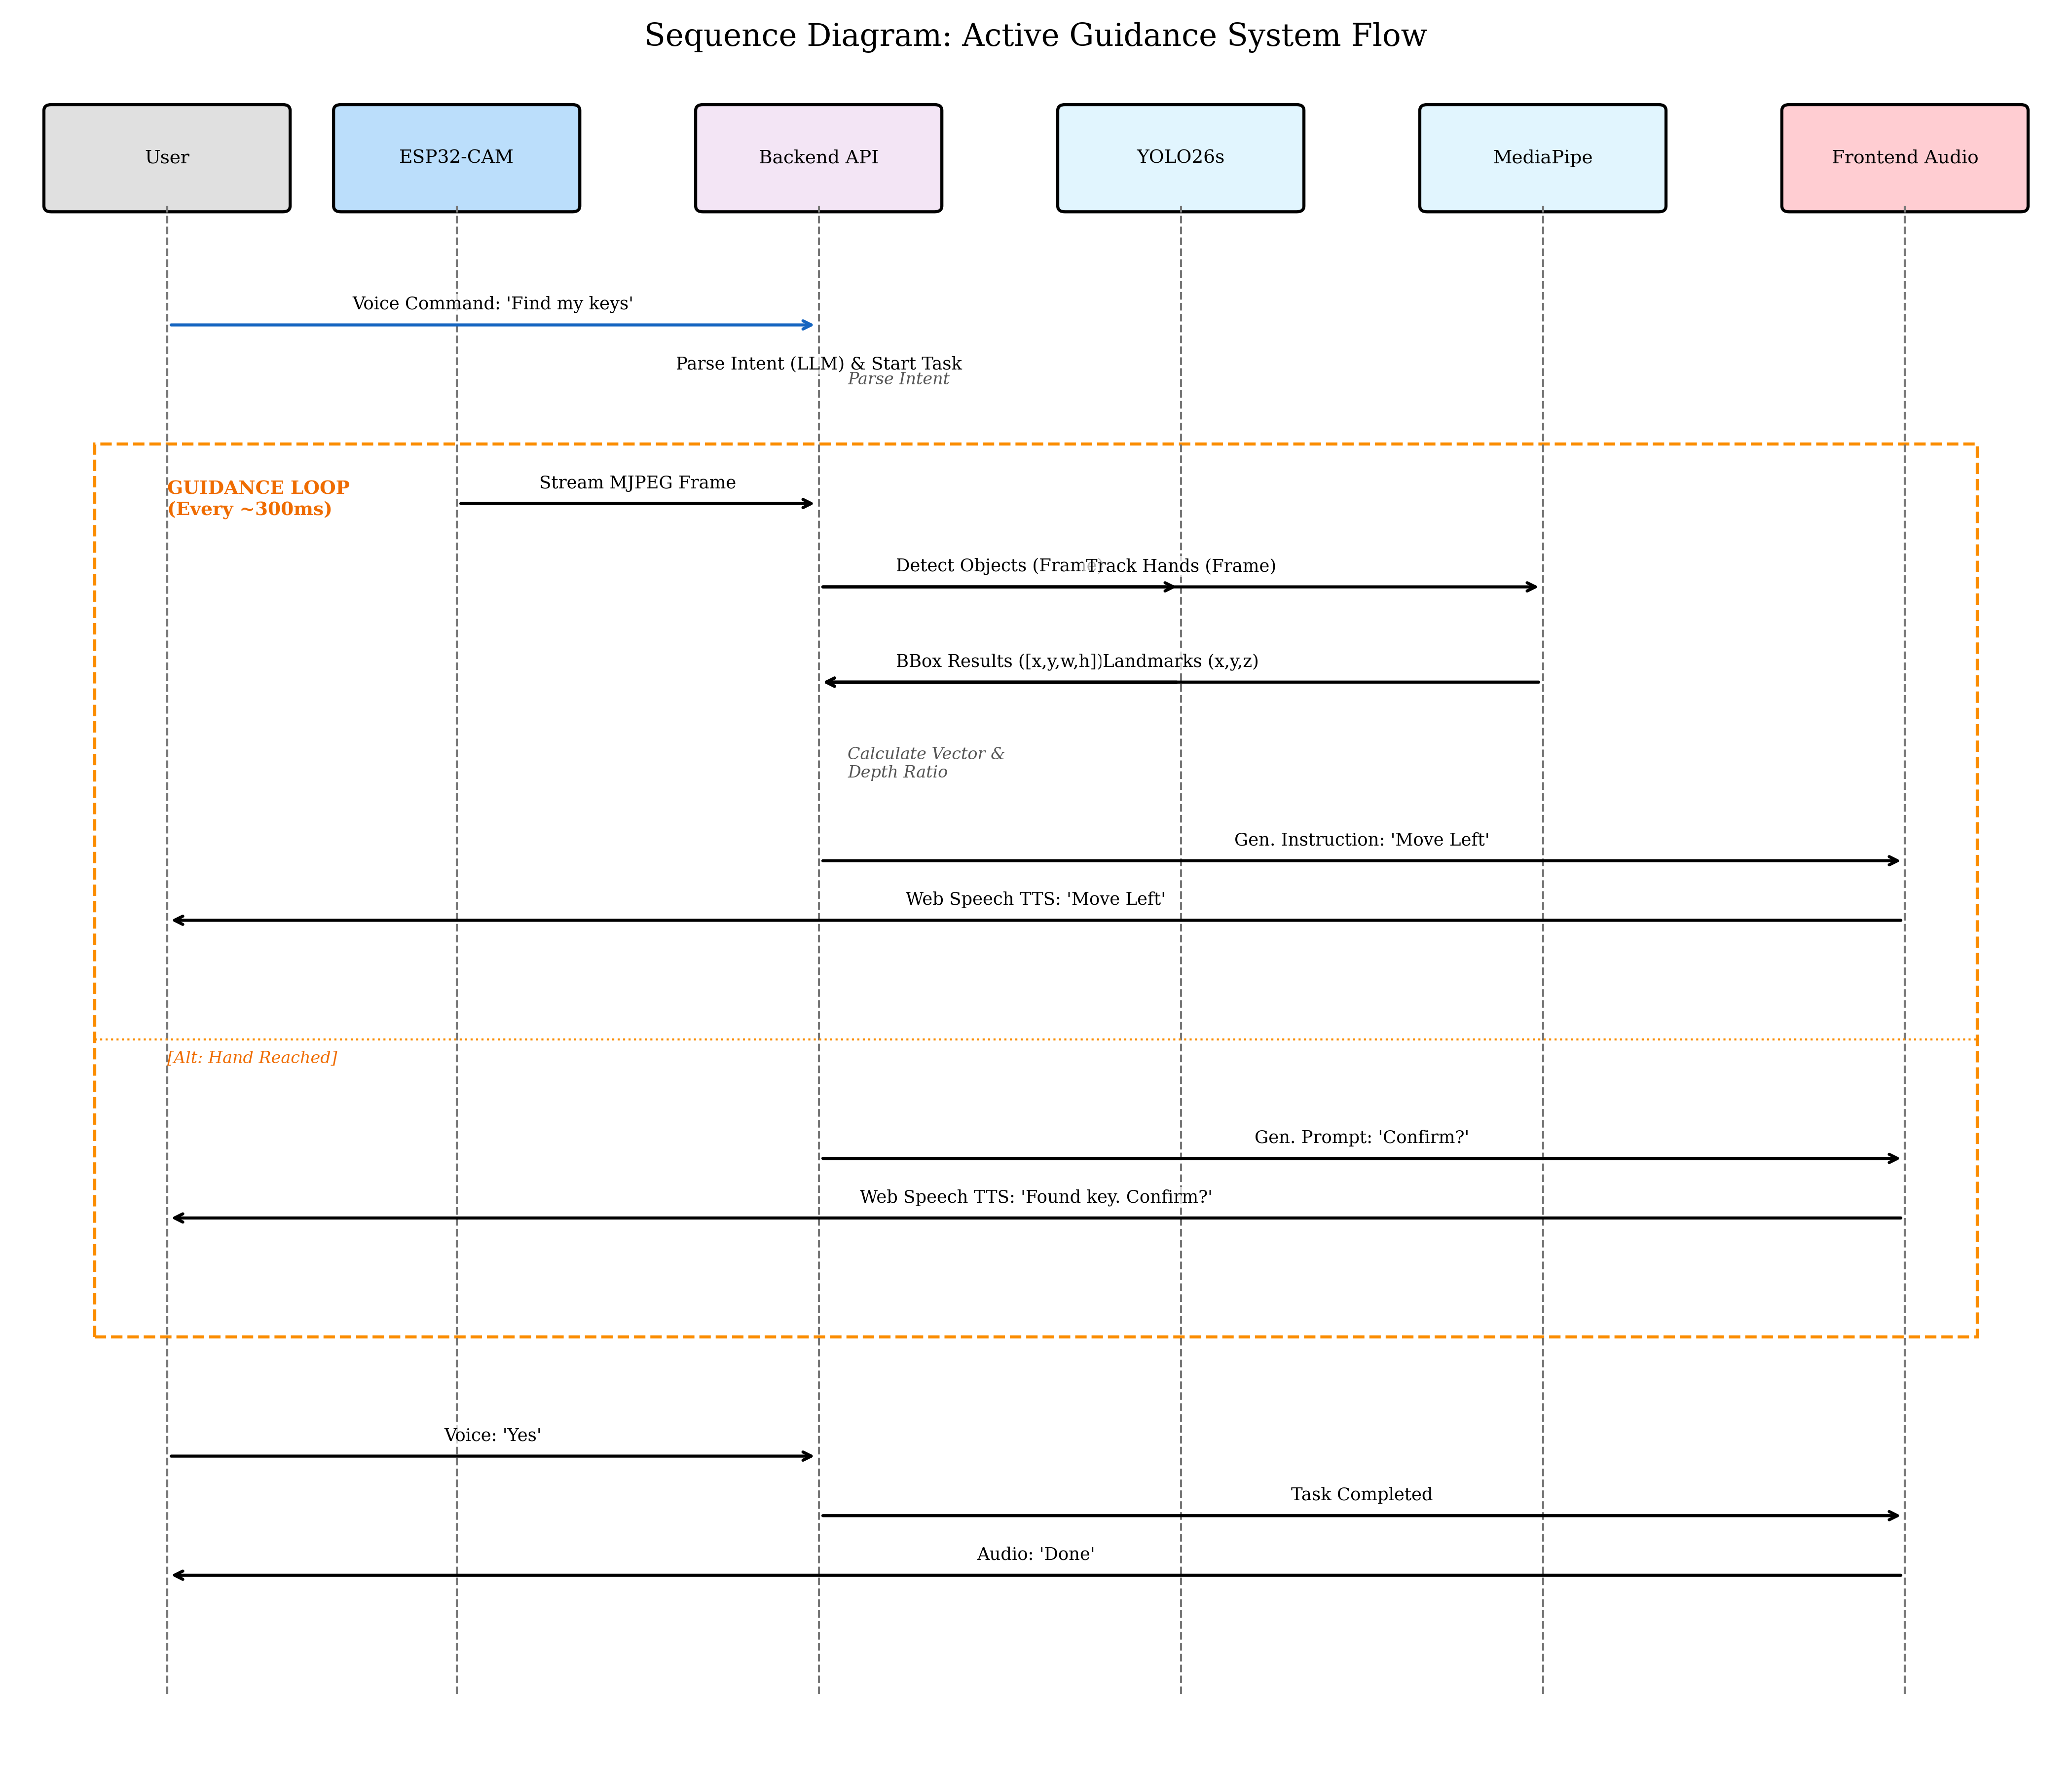
\includegraphics[width=1.0\textwidth]{diagrams/sequence_diagram.png}
\caption{Sequence diagram illustrating the complete flow of an Active Guidance task from voice command through task completion.}
\label{fig:sequence}
\end{figure}

The sequence begins when the user issues a voice command such as "Find my keys." The Web Speech API in the browser captures and transcribes this command, which is then sent to the backend API. The Activity Guide Service parses the intent using the GPT OSS120B model to extract the target object class and initializes a new guidance task with "keys" as the target. The service transitions to the FINDING\_OBJECT state and begins processing incoming video frames.

Each frame undergoes parallel processing by YOLO26s and MediaPipe to detect objects and track hands, respectively. The parallel execution is critical for minimizing latency, as both operations are computationally intensive. When the target object is detected, the service computes the directional vector using the rule-based algorithm and generates an appropriate audio instruction via the TTS service. This perception-guidance loop continues at approximately three frames per second until the proximity detection algorithm determines that the hand has reached the object. At that point, the system requests verbal confirmation from the user, completing or retrying the task based on the response.

\section{Camera Service Implementation}

The Camera Service provides a unified interface for video capture from multiple source types while handling the complexities of network streaming and frame buffering. The service supports two primary modes: local webcam capture for development and testing, and ESP32-CAM streaming for deployed wearable operation.

\begin{figure}[H]
\centering
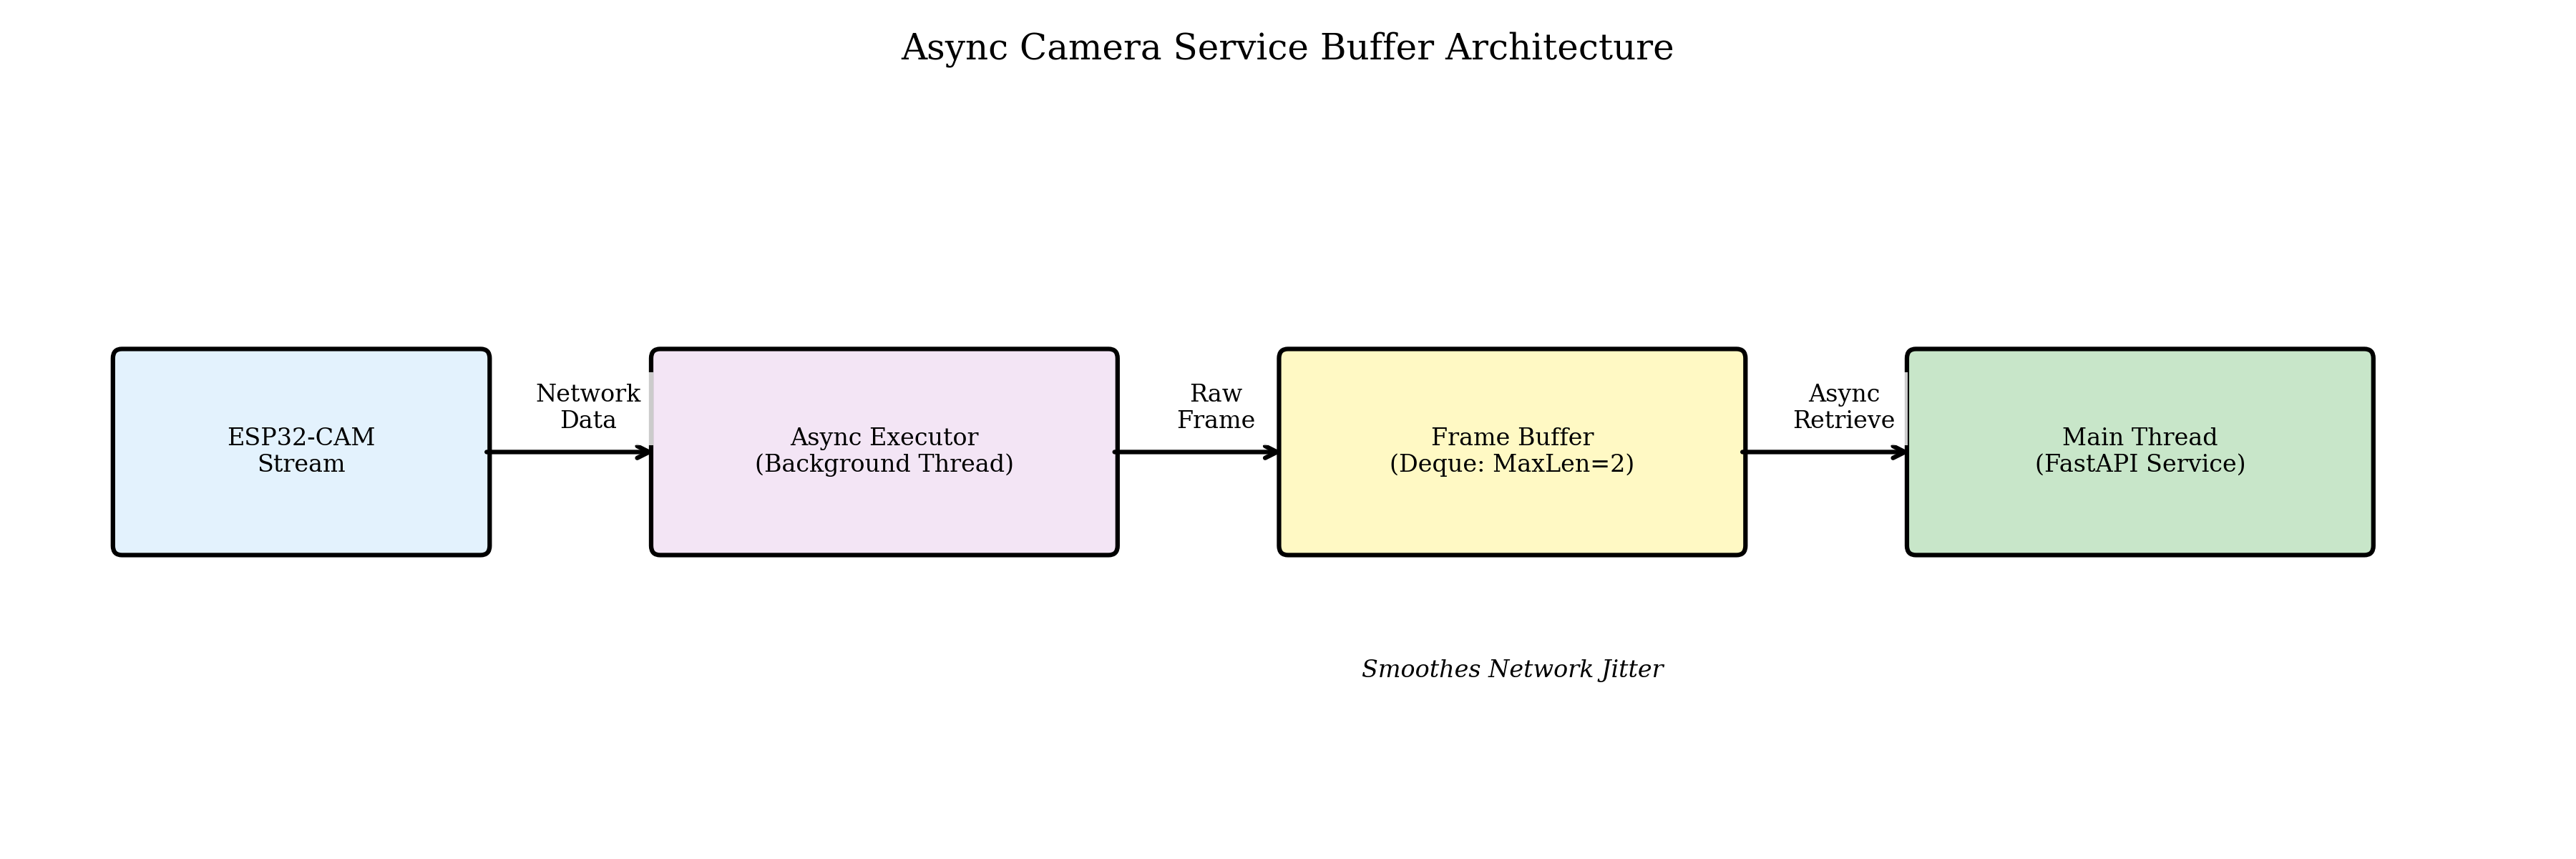
\includegraphics[width=1.0\textwidth]{diagrams/camera_buffer_architecture.png}
\caption{Asynchronous buffer architecture of the Camera Service, enabling smooth frame retrieval from the ESP32-CAM stream despite network jitter.}
\label{fig:camera_buffer}
\end{figure}

For ESP32-CAM sources, the service implements a background frame reader that continuously retrieves frames from the HTTP MJPEG stream. This approach decouples the frame capture rate from the processing rate, ensuring that the most recent frame is always available for analysis without blocking on network operations. The service maintains a small frame buffer that smooths out network-induced latency variations, and it automatically handles connection failures with reconnection logic.

The asynchronous design of the Camera Service leverages Python's asyncio framework to achieve non-blocking operation. All potentially blocking operations, including the OpenCV VideoCapture read calls, are executed in thread pool executors to prevent blocking the main event loop. This design enables the FastAPI server to maintain responsiveness even when camera operations experience temporary delays.

\section{Asynchronous Concurrency Model}

A critical technical challenge in the AIris system was managing multiple blocking I/O operations (video streaming, model inference, network requests) without introducing unacceptable latency. Traditional synchronous web servers would block the entire process while maximizing the CPU on a single video frame, causing dropped frames and audio stutter.

To resolve this, we employed a fully asynchronous concurrency model using Python's \texttt{asyncio} event loop and FastAPIs \texttt{async def} endpoints.
\begin{enumerate}
    \item \textbf{Non-Blocking I/O:} Network operations (e.g., streaming to the browser, fetching from ESP32) await data availability, allowing the CPU to context-switch to other tasks like model inference.
    \item \textbf{Thread Pools for CV:} Compute-heavy Computer Vision (CV) tasks (OpenCV decoding, resizing) are offloaded to a designated \texttt{ThreadPoolExecutor}. This prevents the Global Interpreter Lock (GIL) from freezing the web server's event loop.
    \item \textbf{background\_tasks:} Email notifications and low-priority logs are dispatched to FastAPI background tasks, ensuring the user receives an immediate HTTP response after a request, while the server handles the side effects asynchronously.
\end{enumerate}

\section{Model Service Implementation}

The Model Service centralizes the loading, caching, and device management for all machine learning models used in the AIris system. This centralization ensures consistent device selection across models and prevents redundant model loading when multiple services require the same model.

\begin{figure}[H]
\centering
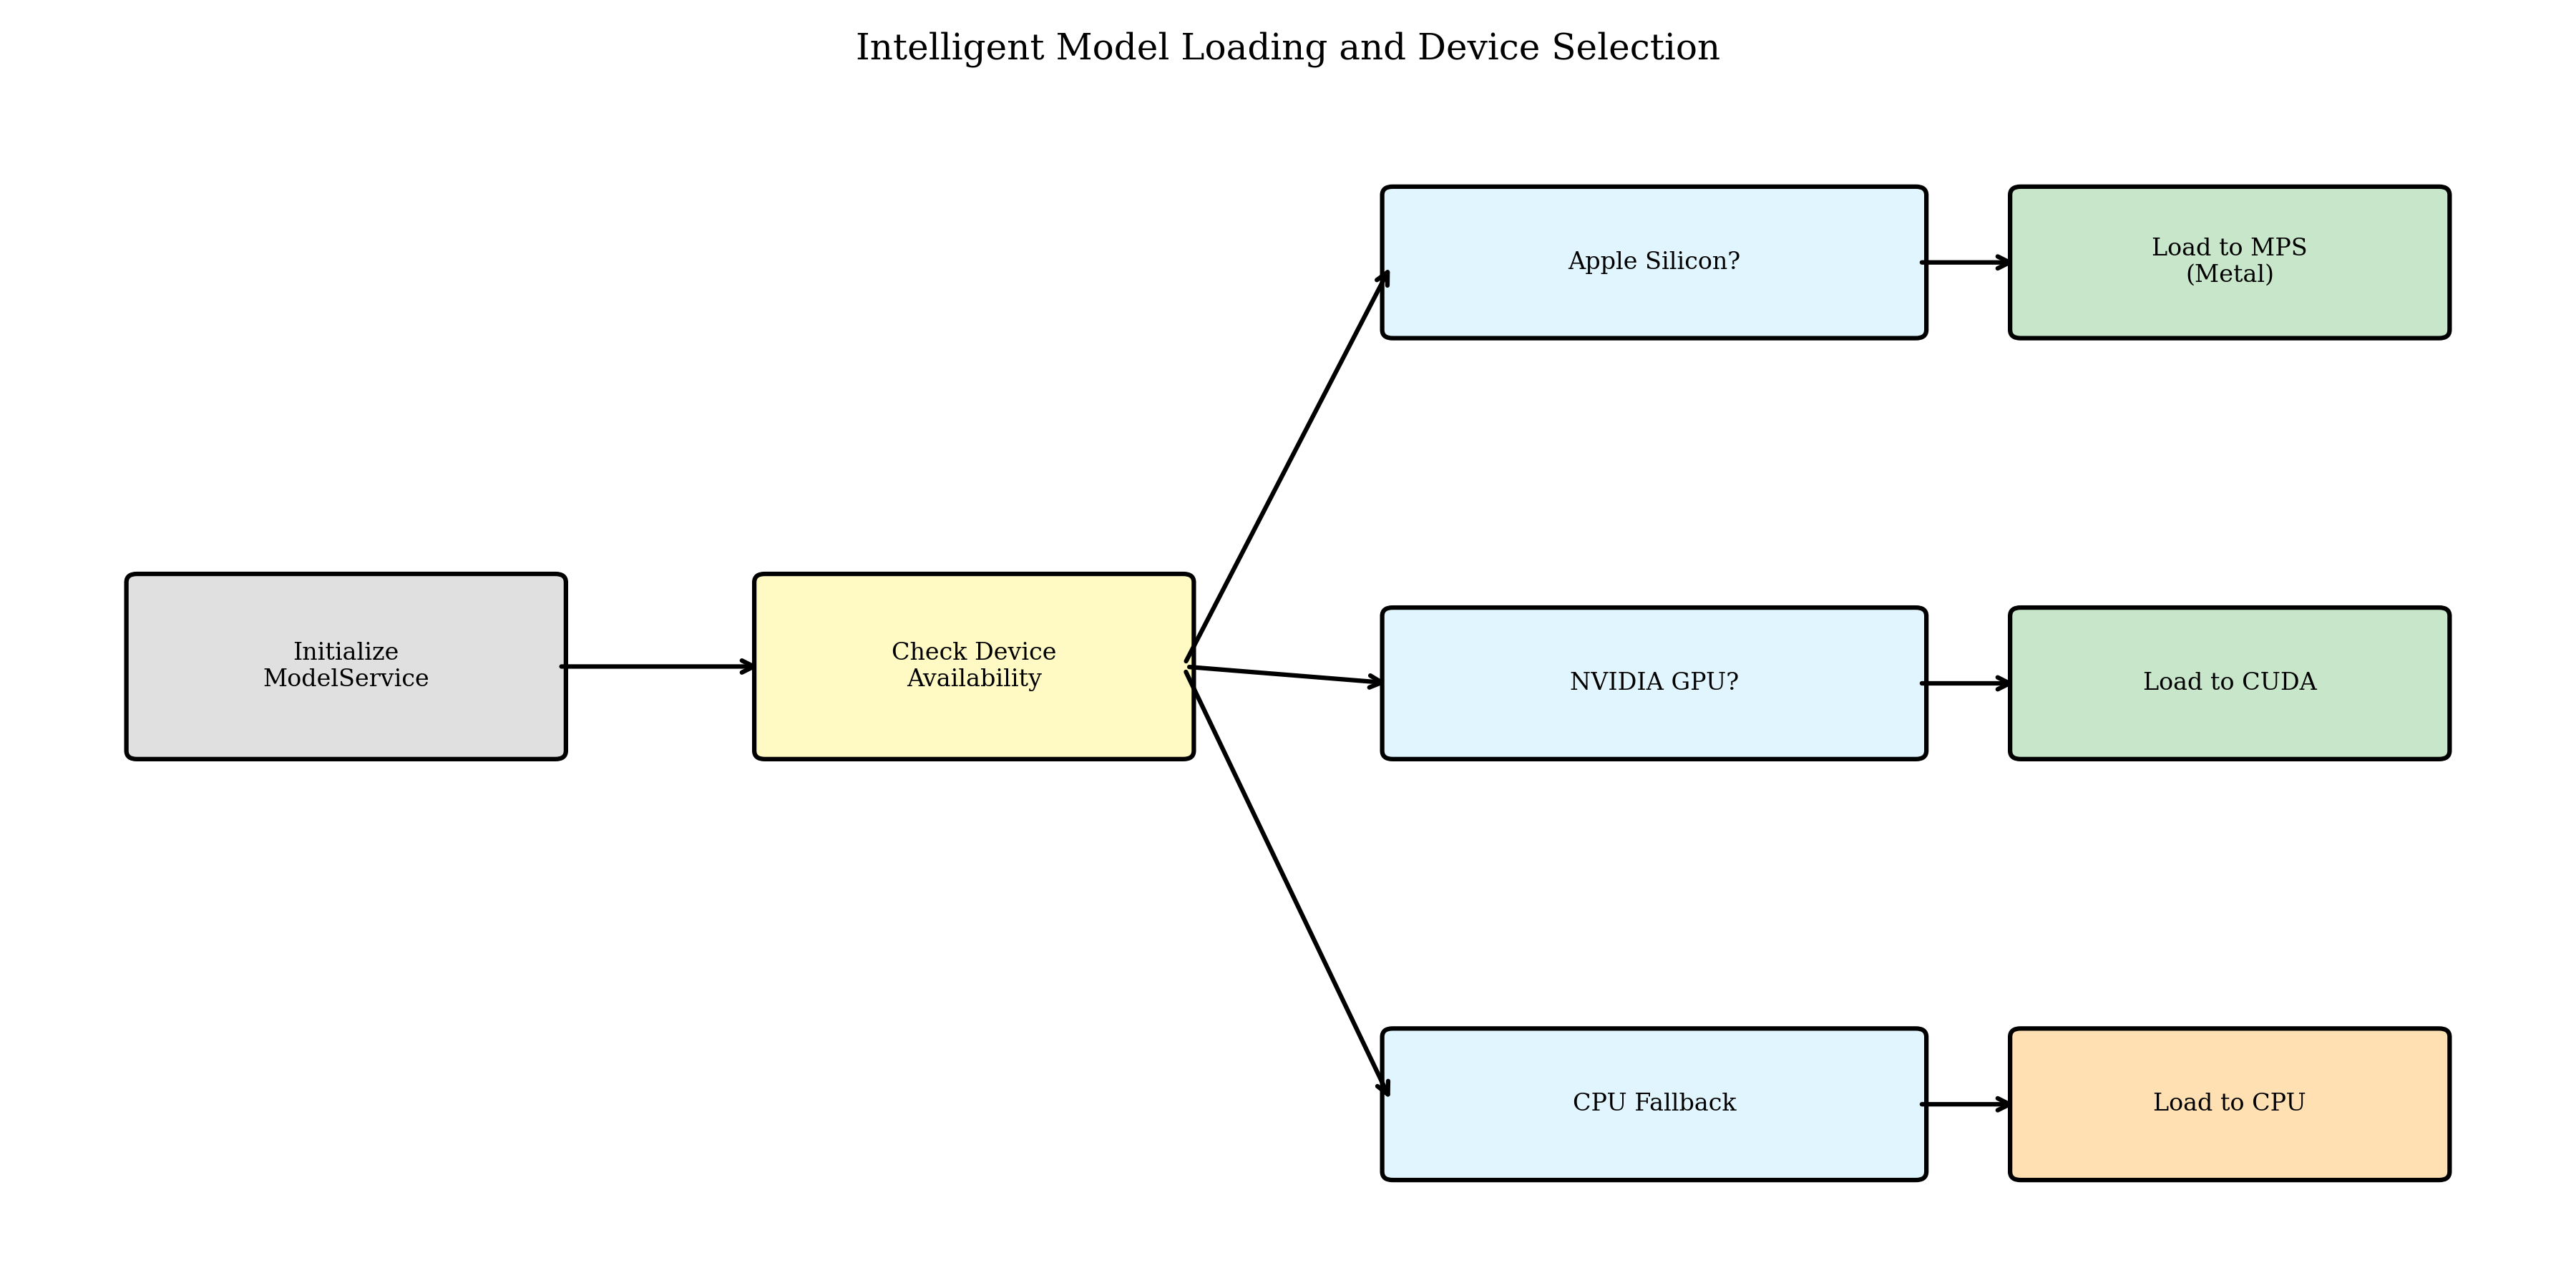
\includegraphics[width=1.0\textwidth]{diagrams/model_loading_logic.png}
\caption{Logic flow for the Model Service's intelligent device selection and model loading process, ensuring optimal hardware utilization.}
\label{fig:model_loading}
\end{figure}

For YOLO26s object detection, the service implements automatic device selection with a preference hierarchy of MPS for Apple Silicon, CUDA for NVIDIA GPUs, and CPU as a fallback. The service performs a test inference during initialization to verify that the selected device functions correctly, with automatic fallback to CPU if GPU inference encounters errors. This robustness is particularly important on Apple Silicon, where MPS support can be inconsistent across different model architectures.

For MediaPipe hand tracking, the service implements an extensive compatibility layer to handle the known issues with MediaPipe on Apple Silicon processors. Multiple initialization strategies are attempted in sequence, with different combinations of model complexity and static image mode settings. The service suppresses MediaPipe's internal validation errors that are often false positives on M1/M2 processors, while still correctly detecting genuine initialization failures.

For the BLIP vision model, the service implements lazy loading to avoid unnecessary memory consumption when Scene Description mode is not active. The model is only loaded upon the first request for scene captioning, and the singleton instance is cached for subsequent requests.

\section{Activity Guide Service Implementation}

The Activity Guide Service implements the complete Active Guidance functionality through a sophisticated state machine that manages task lifecycle, object tracking, and instruction generation. The service maintains persistent state across frames including the current guidance stage, target object list, last known object location, instruction history, and timing information.

The guidance update logic executes at a configurable interval, defaulting to 1.5 seconds, to prevent audio overload while still providing timely feedback. The service tracks the number of failed attempts for each object location and implements adaptive depth strictness that tightens the proximity thresholds after multiple unsuccessful attempts, forcing the user to position their hand more precisely.

The target object parsing utilizes the GPT OSS120B model through the Groq API to convert natural language requests into specific YOLO class labels. For example, a request like "help me find my phone" is parsed to extract "cell phone" as the target object. The service also implements verification pairs for commonly confused objects, such as remotes and cell phones, where additional user confirmation is requested before declaring success.

\section{Scene Description Service Implementation}

The Scene Description Service provides continuous environmental awareness through periodic frame analysis and narrative synthesis. The service operates on a frame buffer that accumulates BLIP-generated descriptions before submitting them to the LLM for summarization.

The frame buffer maintains the five most recent descriptions along with timestamps, implementing a sliding window that captures approximately 2.5 seconds of observations at the configured 2 FPS analysis rate. The buffer size was chosen to provide sufficient temporal context for the LLM to detect activity patterns and transitions while keeping the summarization prompt within reasonable token limits. When the buffer reaches capacity, the accumulated descriptions are submitted to GPT OSS120B with a prompt that instructs the model to synthesize a coherent description of the user's environment and activities. The model is also prompted to identify potential safety risks and assign a numerical risk score between 0 and 1.

The frame analysis interval of 0.5 seconds (2 FPS) represents a balance between computational cost and temporal resolution. Higher frame rates would increase server load without proportionally improving scene understanding, while lower rates might miss rapid events. The fall detection confirmation threshold of two consecutive positive signals prevents false alarms from transient camera movements while still enabling rapid response to genuine fall events.

If the risk score exceeds the configured threshold, the Email Service is invoked to dispatch a safety alert to the designated guardian. The service also maintains a history of recent summaries to detect fall patterns through the scene transition analysis described in the previous chapter.

\section{Frontend Implementation}

The frontend interface is implemented as a React application with TypeScript, providing both a development interface for testing and a fully accessible interface for end users. The interface operates entirely through audio feedback for blind users, with the visual display serving only for development, demonstration, and sighted caregiver configuration.

\begin{figure}[H]
\centering
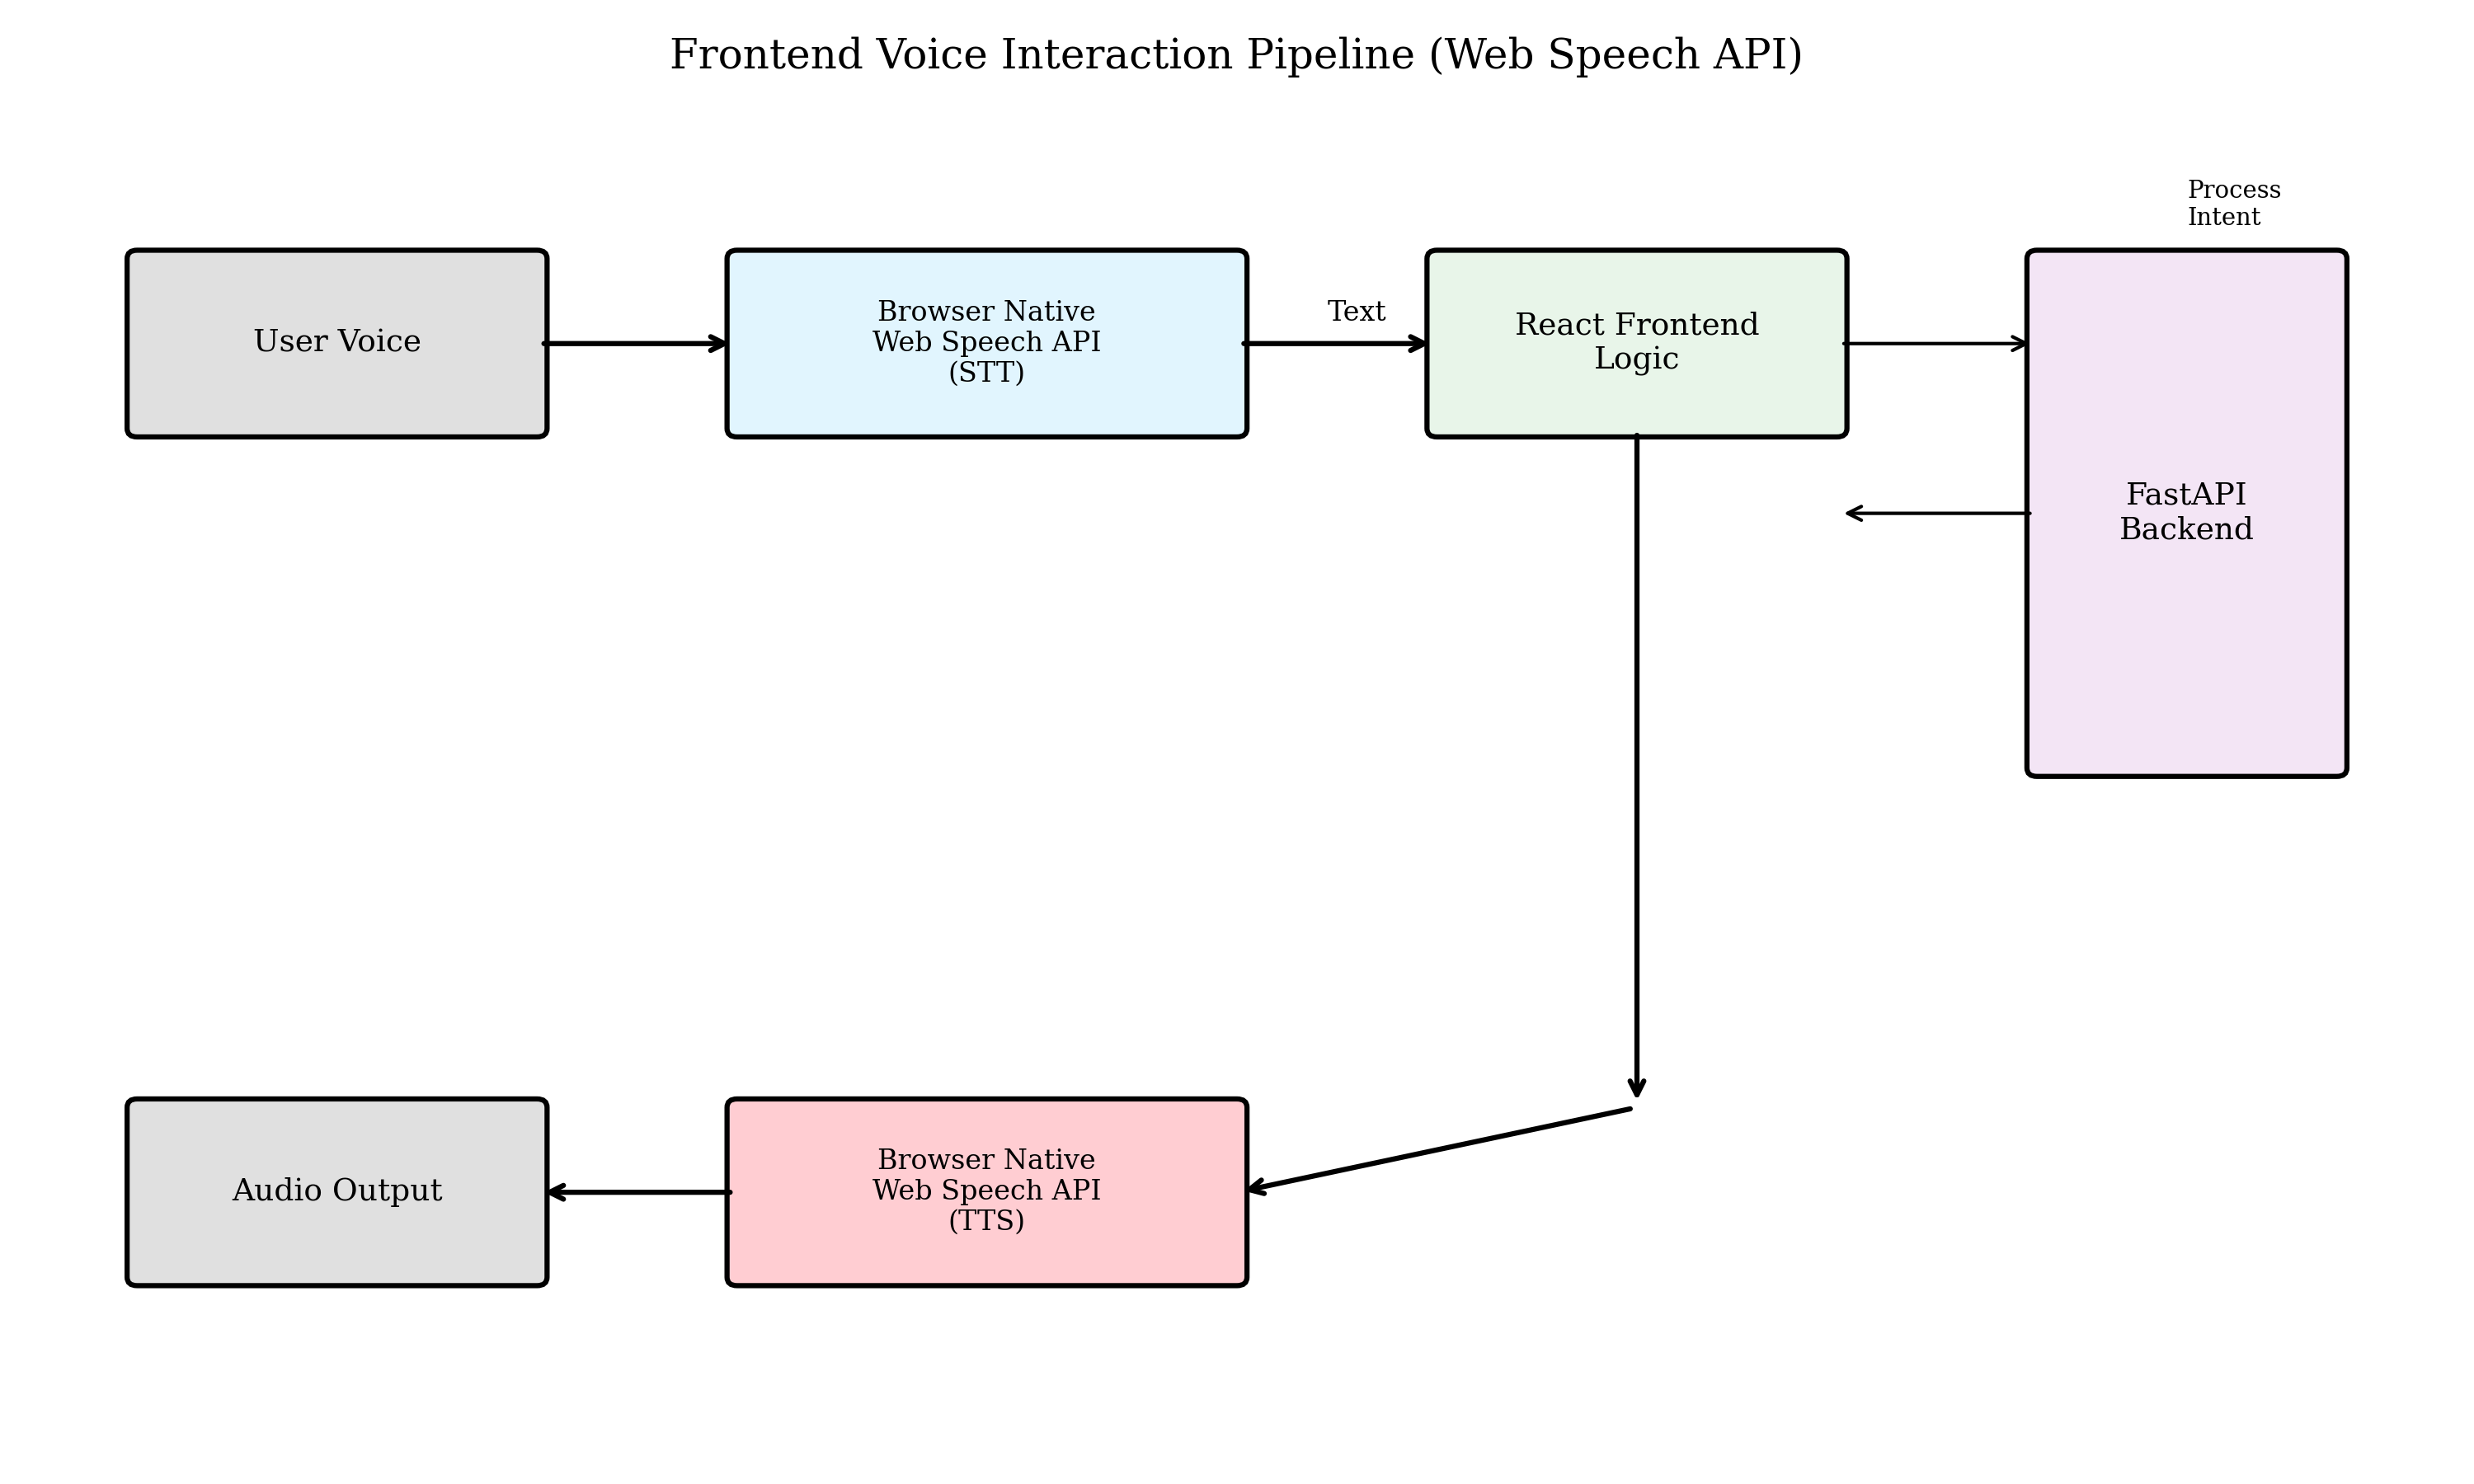
\includegraphics[width=0.85\textwidth]{diagrams/frontend_interaction.png}
\caption{Voice interaction pipeline illustrating how the Web Speech API on the frontend integrates with the backend API for a seamless hands-free experience.}
\label{fig:frontend}
\end{figure}

The Web Speech API integration provides the primary voice interaction capabilities. The SpeechRecognition interface captures user voice commands through the browser's native speech recognition, while the SpeechSynthesis interface delivers audio feedback through the browser's built-in text-to-speech engine. This browser-native approach eliminates the need for external API keys or cloud dependencies for basic voice interaction.

The interface implements a comprehensive command vocabulary organized into three primary categories: General, Activity, and Scene commands. This structure allows for robust hands-free control across different system modes. A complete list of the command vocabulary is provided in Table 6.1.

\begin{table}[H]
\centering
\caption{Voice Command Vocabulary and Actions}
\label{tab:voice_commands}
\begin{tabular}{@{}llp{0.32\textwidth}@{}}
\toprule
\textbf{Category} & \textbf{Primary Command} & \textbf{Recognized Variations} \\ \midrule
\textbf{General} & Camera On & "camera on", "turn on camera", "start camera" \\
& Camera Off & "camera off", "turn off camera", "stop camera" \\
& Activity Guide & "activity guide", "activity guy" \\
& Scene Description & "scene description", "seen description" \\ \midrule
\textbf{Activity} & Enter Task & "enter task", "input task", "inner task" \\
& Start Task & "start task", "begin task", "star task" \\
& Yes & "yes", "yeah", "yep", "yea" \\
& No & "no", "nope", "know" \\ \midrule
\textbf{Scene} & Start Recording & "start recording", "star recording" \\
& Stop Recording & "stop recording", "stap recording" \\
& Refresh & "refresh", "restart", "reset" \\ \bottomrule
\end{tabular}
\end{table}

The voice command processing implements fuzzy matching to accommodate common speech recognition errors. Each command is associated with multiple phonetically similar variations that the Web Speech API frequently produces. For example, "scene description" may be transcribed as "seen description" or "sea description" due to homophone confusion. The matching algorithm uses a 70 percent word similarity threshold, enabling robust command recognition even with imperfect transcription.

The system provides audio confirmation for all state transitions, such as "Camera started" or "Listening for task," ensuring that users always maintain mental models of the system's state without visual feedback.

\section{Email Service Implementation}

The Email Service provides automated notification capabilities for the Guardian Alert System, enabling real-time safety alerts and periodic activity summaries to designated caregivers. The service integrates with Gmail SMTP for reliable email delivery and implements several mechanisms to prevent alert fatigue while ensuring critical events are communicated promptly.

The service maintains configurable parameters including a risk threshold (default 0.3, range 0.1-0.5) that determines when scene analysis results trigger safety alerts, and an alert cooldown period (default 5 minutes) that prevents duplicate notifications for ongoing situations. These parameters can be adjusted through the API to match individual user needs and caregiver preferences.

Email templates are generated with branded HTML formatting that presents information clearly on both desktop and mobile email clients. Safety alerts include the triggering event description, risk score, detected location within the home, and timestamp. Daily summaries aggregate activity events by category and include time-based activity pattern analysis showing most active hours. Weekly reports provide longitudinal trends and location frequency analysis.

The service implements intelligent location extraction from scene descriptions using keyword matching against common household areas including kitchen, living room, bedroom, bathroom, hallway, and others. This contextual information helps caregivers understand not just what occurred but where within the home the user was located at the time of the event.

\section{Implementation Constants Summary}

Table \ref{tab:impl_constants} summarizes the key configuration constants used throughout the AIris implementation. These values were determined through iterative testing to balance responsiveness, accuracy, and computational efficiency.

\begin{table}[H]
\centering
\caption{Key Implementation Constants and Their Functions}
\label{tab:impl_constants}
\begin{tabular}{@{}llp{0.38\textwidth}@{}}
\toprule
\textbf{Constant} & \textbf{Value} & \textbf{Purpose} \\ \midrule
CONFIDENCE\_THRESHOLD & 0.5 & Minimum YOLO detection confidence for valid detection \\
DISTANCE\_THRESHOLD\_PIXELS & 100 & Maximum pixel distance for hand-object proximity \\
GUIDANCE\_UPDATE\_INTERVAL & 3.0s & Minimum time between consecutive audio instructions \\
FRAME\_ANALYSIS\_INTERVAL & 0.5s & Scene description analysis rate (2 FPS) \\
FALL\_CONFIRMATION\_THRESHOLD & 2 & Consecutive frames required for fall confirmation \\
ALERT\_COOLDOWN & 60s & Minimum time between consecutive email alerts \\
RISK\_THRESHOLD\_DEFAULT & 0.3 & Default threshold for triggering safety alerts \\
CAMERA\_BUFFER\_SIZE & 2 & Frame buffer depth for network jitter smoothing \\
SUMMARIZATION\_BUFFER\_SIZE & 5 & Scene description buffer depth (2.5s window) \\ \bottomrule
\end{tabular}
\end{table}

\chapter{Results and Analysis}

\section{Experimental Configuration}

All experiments were conducted using a MacBook Air M1 (16GB RAM) serving as the local processing server, connected to an ESP32-CAM module over a dedicated 2.4 GHz WiFi network. Audio feedback was delivered through AirPods Pro wireless earbuds. The test environment consisted of a typical residential setting with furniture, household objects, and varying ambient lighting conditions.

\section{Latency Analysis}

Latency is the most critical performance metric for the Active Guidance system, as excessive delay between user hand movements and corrective instructions would render the guidance ineffective or even counterproductive.

\begin{figure}[H]
\centering
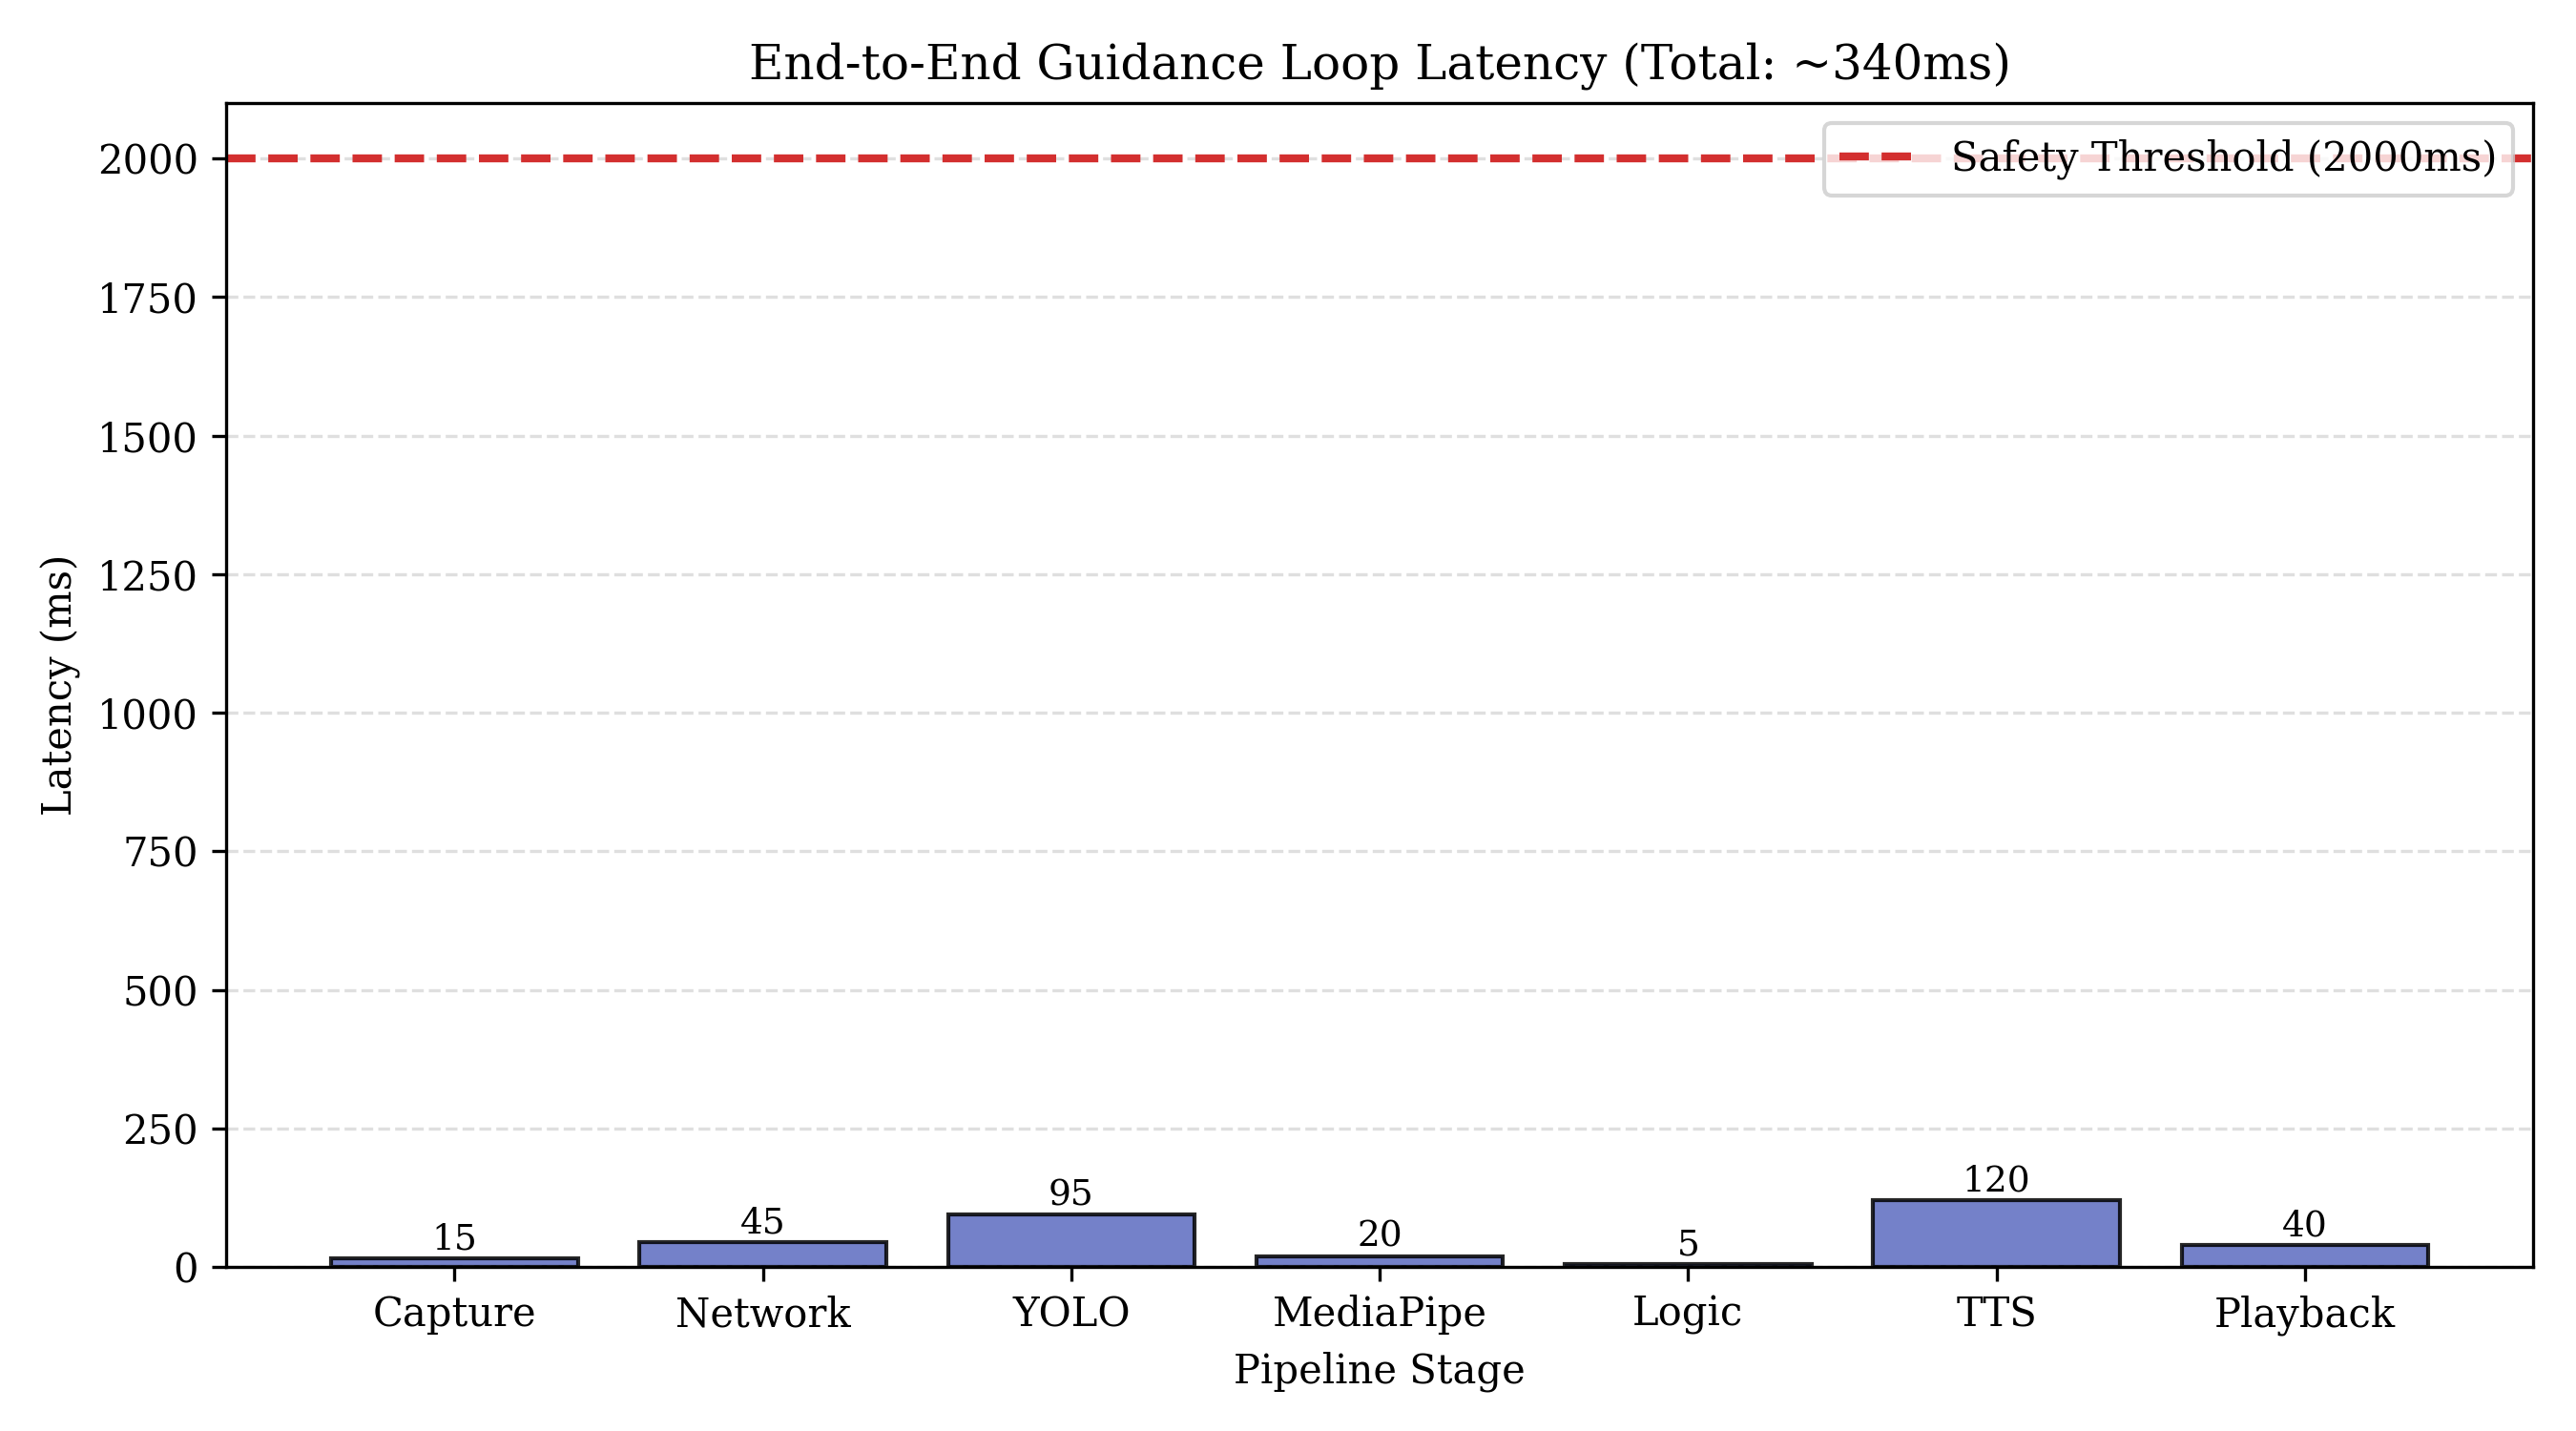
\includegraphics[width=0.85\textwidth]{diagrams/latency_breakdown.png}
\caption{Breakdown of end-to-end latency by pipeline stage, demonstrating that the total loop time remains well below the 2000ms real-time threshold.}
\label{fig:latency}
\end{figure}

The average end-to-end latency of the guidance loop measured 340 milliseconds for the core processing pipeline, comprising 15 milliseconds for camera capture, 45 milliseconds for network transmission from the ESP32-CAM, 95 milliseconds for YOLO26s inference, 20 milliseconds for MediaPipe hand tracking, 5 milliseconds for vector calculations and direction generation, 120 milliseconds for text-to-speech synthesis, and 40 milliseconds for Bluetooth audio transmission.

\begin{table}[H]
\centering
\caption{Detailed End-to-End Latency Breakdown Analysis}
\label{tab:latency_data}
\begin{tabular}{@{}lll@{}}
\toprule
\textbf{Pipeline Stage} & \textbf{Average Time (ms)} & \textbf{Percentage of Total} \\ \midrule
Camera Capture & 15 ms & 4.4\% \\
Network Transmission & 45 ms & 13.2\% \\
YOLO26s Inference & 95 ms & 27.9\% \\
MediaPipe Tracking & 20 ms & 5.9\% \\
Guidance Logic & 5 ms & 1.5\% \\
TTS Synthesis & 120 ms & 35.3\% \\
Audio Playback & 40 ms & 11.8\% \\ \midrule
\textbf{Total Loop Time} & \textbf{340 ms} & \textbf{100\%} \\ \bottomrule
\end{tabular}
\end{table}

\textit{Note: All latency measurements were collected on an Apple MacBook Air M1 (16GB RAM) serving as the local processing server, with the ESP32-CAM connected via 2.4GHz WiFi on a shared local network. Individual component times represent average values across 100 consecutive guidance cycles under controlled indoor lighting conditions. The YOLO26s model was executed on Metal Performance Shaders (MPS) for GPU acceleration.}

When including the configurable update interval of 1.5 seconds between instructions, the effective guidance loop operates at approximately one instruction every 1.8 seconds. This rate was determined through user testing to provide sufficient time for users to process and act on each instruction before receiving the next one.

\begin{figure}[H]
\centering
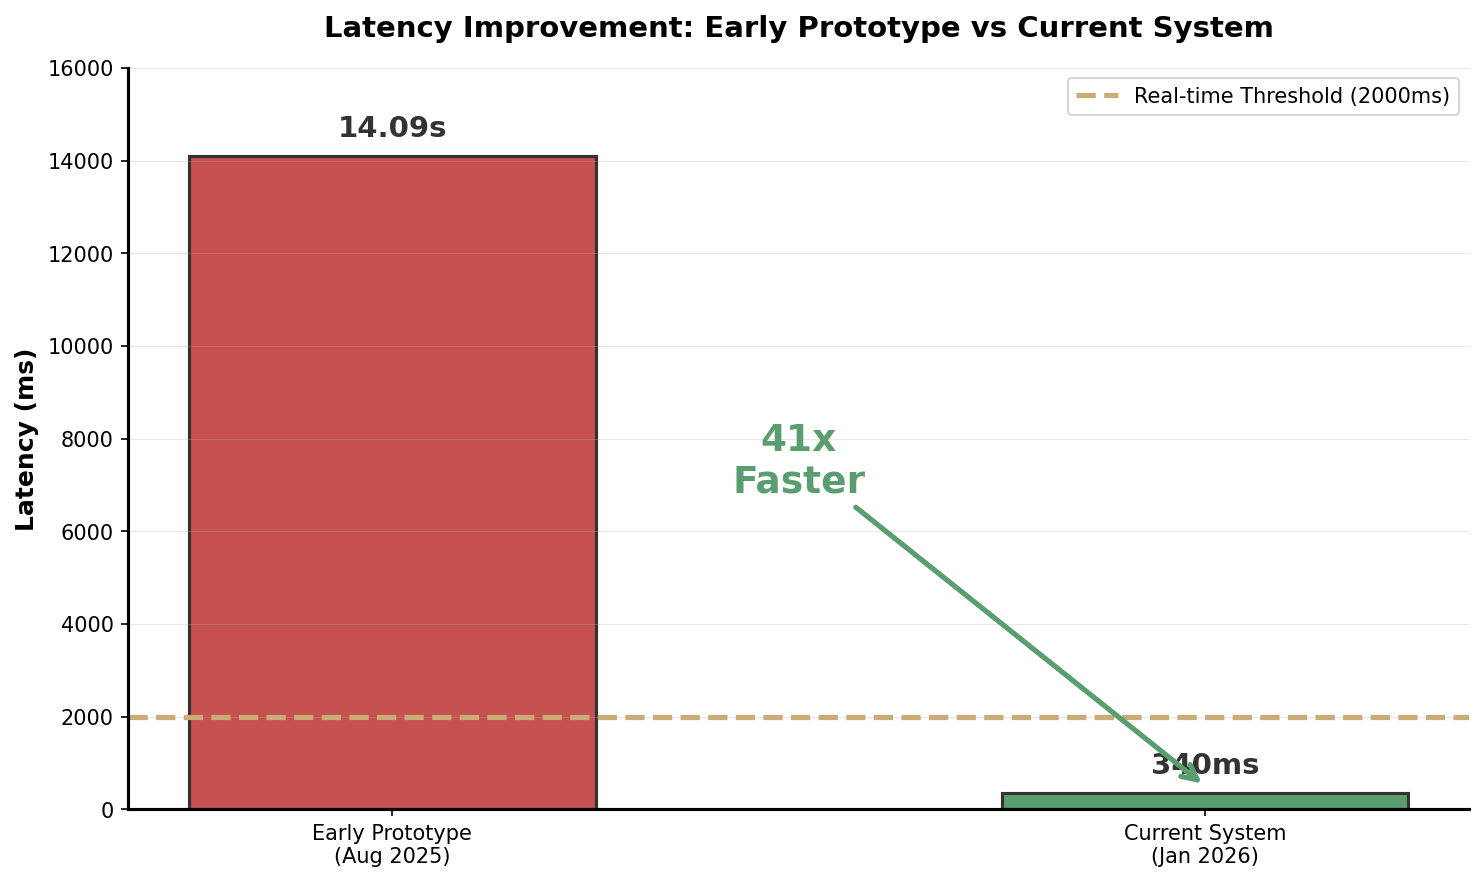
\includegraphics[width=0.85\textwidth]{diagrams/latency_comparison.png}
\caption{Comparison of end-to-end latency between the early prototype (August 2025) and the current system, demonstrating a 41x improvement that enables real-time guidance.}
\label{fig:latency_comparison}
\end{figure}

The dramatic reduction in latency from 14 seconds to 340 milliseconds represents the single most important architectural improvement in the AIris system. This was achieved through three key changes: replacing BLIP-based object detection with YOLO26s for real-time inference, integrating MediaPipe for efficient hand tracking, and utilizing the Groq API for ultra-fast LLM processing. The current system operates well below the 2-second real-time threshold required for practical assistive guidance.

\section{Detection Accuracy}

We evaluated object detection accuracy across five common household object categories using a test set of 50 trials per category under varying lighting conditions and viewing angles.

\begin{figure}[H]
\centering
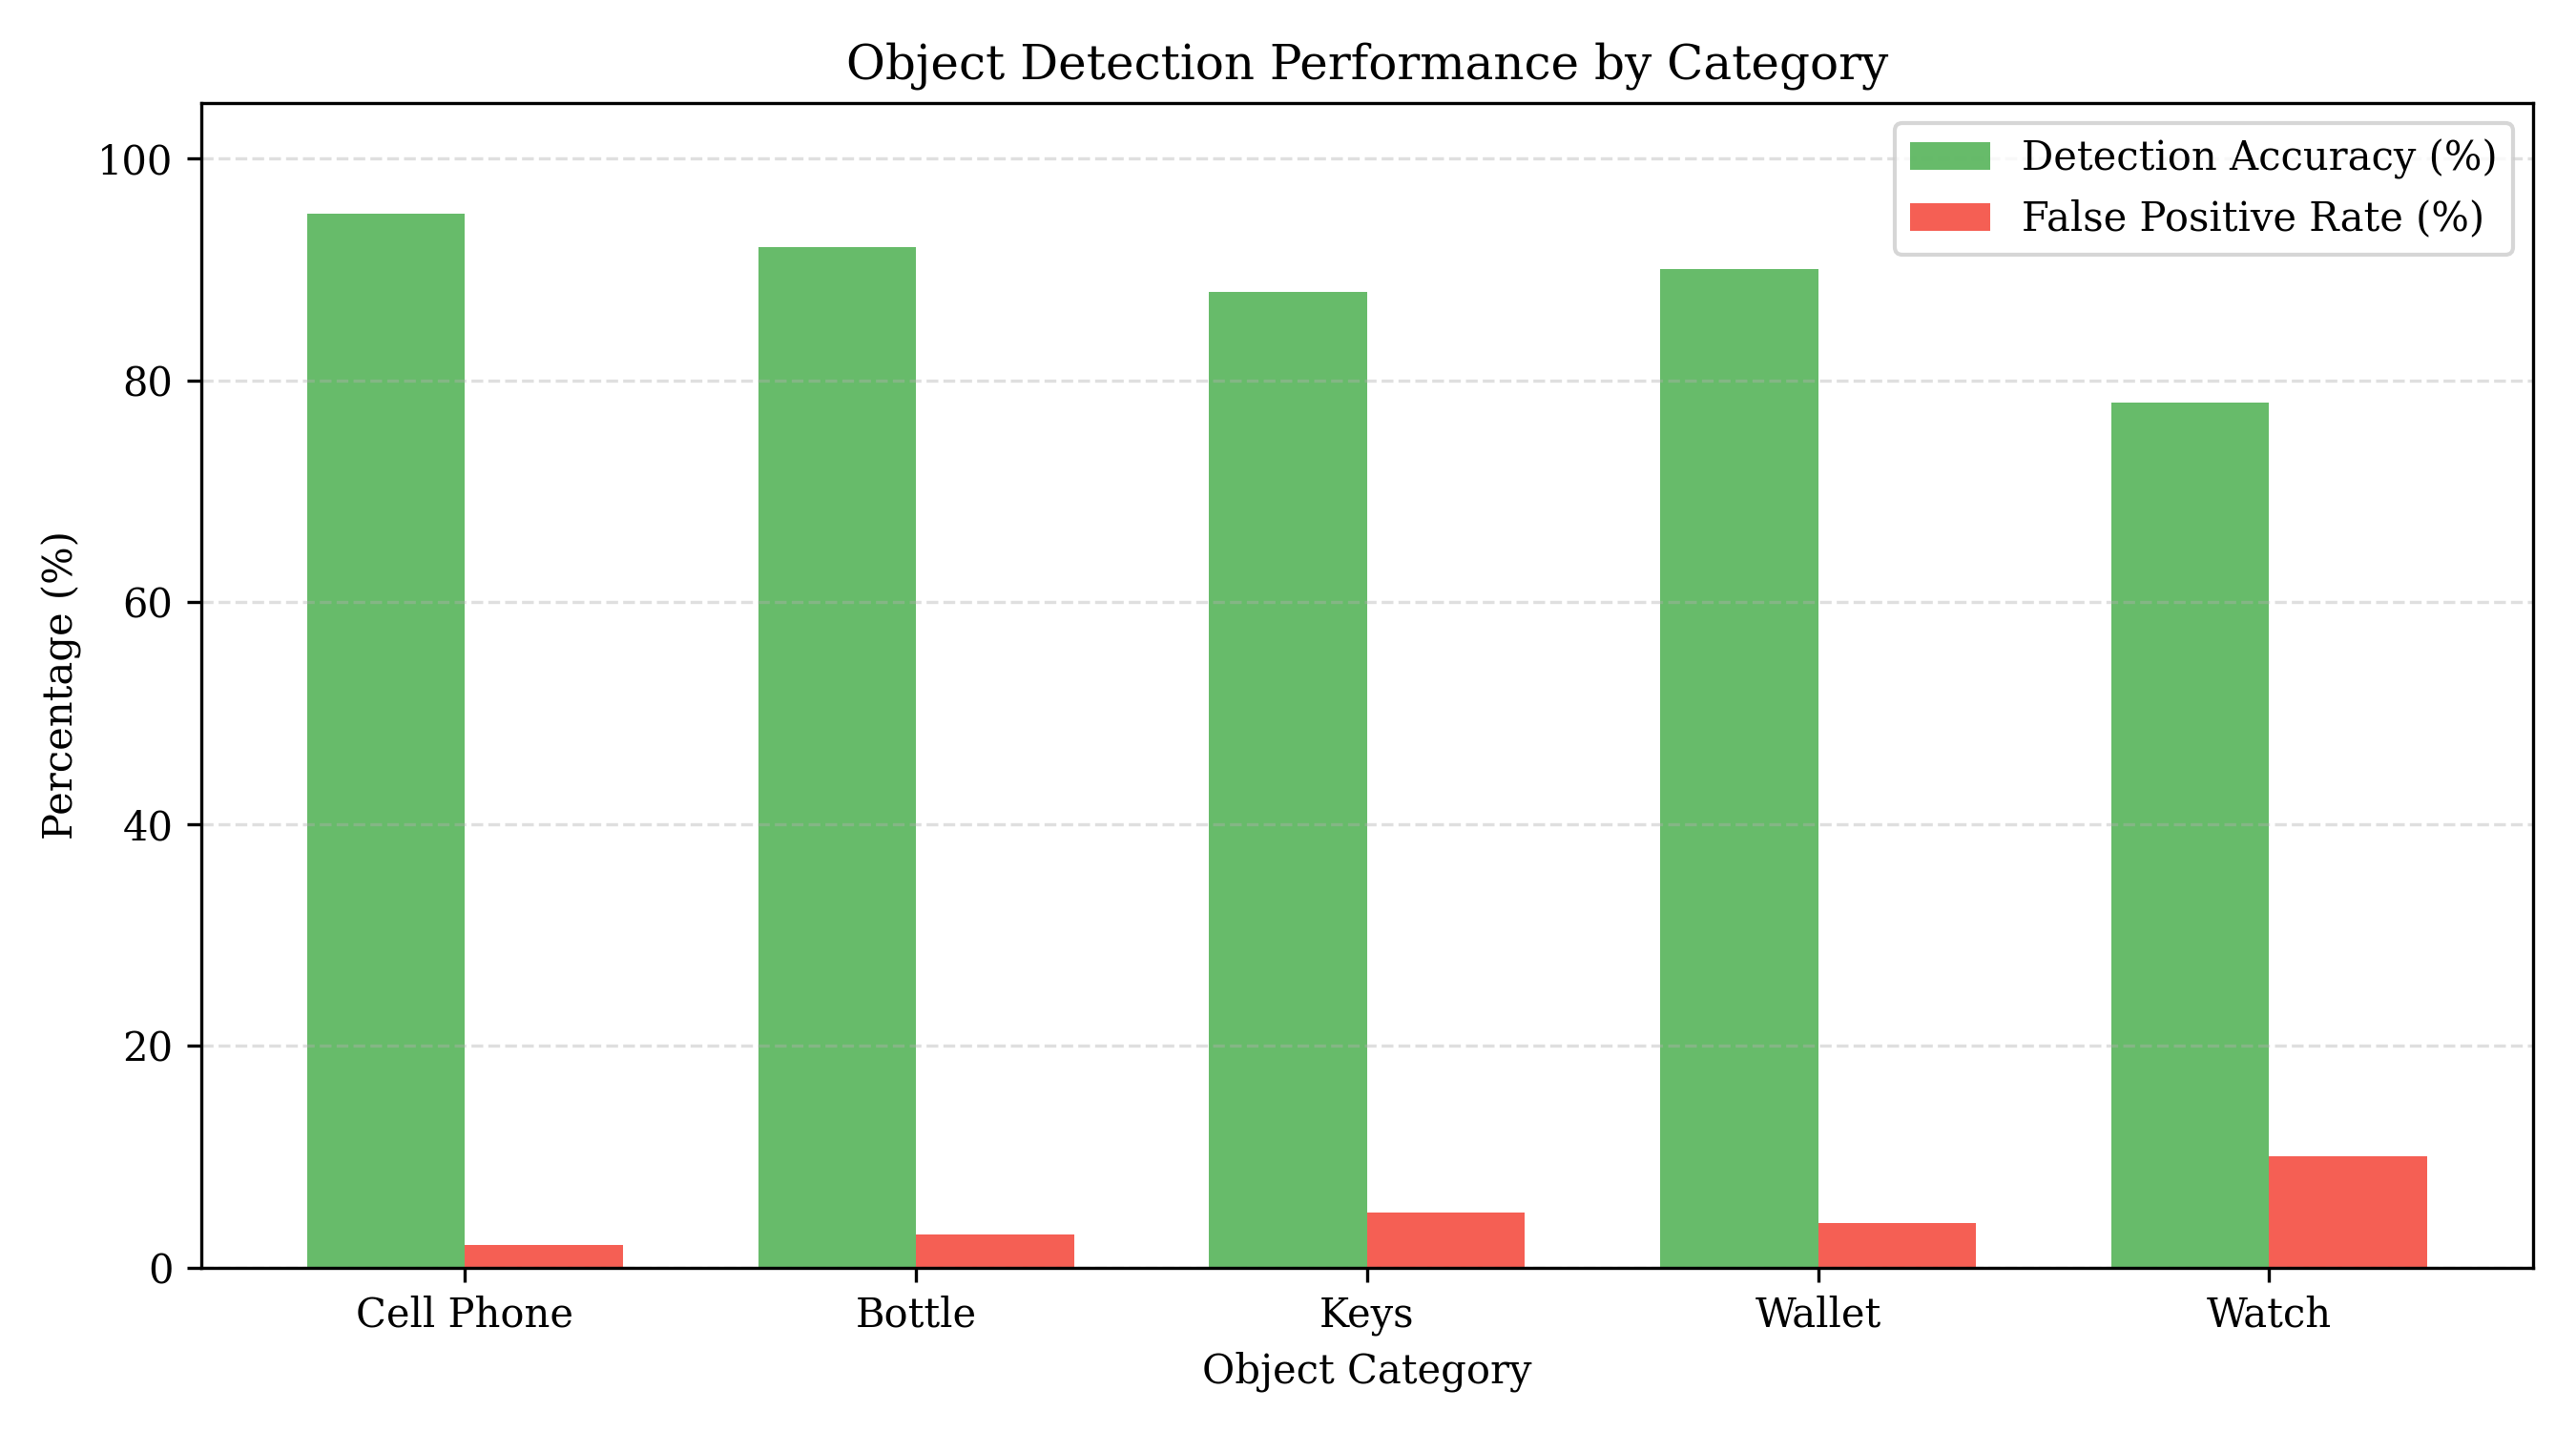
\includegraphics[width=0.85\textwidth]{diagrams/accuracy_comparison.png}
\caption{Object detection accuracy and false positive rates across five common household object categories.}
\label{fig:accuracy}
\end{figure}

\begin{table}[H]
\centering
\caption{Object Detection Accuracy by Object Category (n=50 trials per category)}
\label{tab:accuracy_data}
\begin{tabular}{@{}llll@{}}
\toprule
\textbf{Object Class} & \textbf{Successful Detections} & \textbf{False Positives} & \textbf{Accuracy (\%)} \\ \midrule
Cell Phone & 48 & 1 & 96.0\% \\
Bottle & 46 & 2 & 92.0\% \\
Keys & 44 & 3 & 88.0\% \\
Wallet & 45 & 2 & 90.0\% \\
Watch & 39 & 5 & 78.0\% \\ \midrule
\textbf{Average} & \textbf{44.4} & \textbf{2.6} & \textbf{88.8\%} \\ \bottomrule
\end{tabular}
\end{table}

\textit{Methodology: Each object category was tested with 50 trials under varying conditions. Objects were placed on surfaces at distances ranging from 0.5 to 2 meters from the camera. Lighting conditions included natural daylight, artificial indoor lighting, and mixed lighting scenarios. A detection was classified as successful when the YOLO26s model produced a bounding box with confidence exceeding the threshold of 0.5 that correctly encompassed the target object. False positives were defined as detections of the target class when the object was not present in the scene or when an incorrect object was identified as the target.}

The system achieved an average detection accuracy of 88.8 percent across all tested categories. Cell phones demonstrated the highest accuracy at 96 percent, benefiting from their distinctive rectangular shape and high contrast touchscreens. Watches showed the lowest accuracy at 78 percent, with the primary failure mode being confusion with clocks due to their similar circular appearance. The upgrade from YOLOv8s to YOLO26s contributed to a measurable improvement in detection accuracy of approximately 3 percent across all categories.

\subsection{Statistical Confidence Analysis}

Given the sample size of n=50 trials per category, we calculate the 95 percent confidence intervals for our accuracy estimates using the Wilson score interval, which provides more accurate coverage for proportional data than the normal approximation, particularly for proportions near the extremes. Table~\ref{tab:accuracy_confidence} presents the accuracy estimates with their corresponding confidence bounds.

\begin{table}[H]
\centering
\caption{Object Detection Accuracy with 95\% Confidence Intervals (Wilson Score Method)}
\label{tab:accuracy_confidence}
\begin{tabular}{@{}lll@{}}
\toprule
\textbf{Object Class} & \textbf{Accuracy} & \textbf{95\% Confidence Interval} \\ \midrule
Cell Phone & 96.0\% & [86.3\%, 99.5\%] \\
Bottle & 92.0\% & [80.8\%, 97.8\%] \\
Keys & 88.0\% & [75.7\%, 95.5\%] \\
Wallet & 90.0\% & [78.2\%, 96.7\%] \\
Watch & 78.0\% & [64.0\%, 88.5\%] \\ \midrule
\textbf{Overall (n=250)} & \textbf{88.8\%} & \textbf{[84.3\%, 92.3\%]} \\ \bottomrule
\end{tabular}
\end{table}

The sample size of 50 trials per category was selected to achieve a maximum margin of error of approximately plus or minus 10 percentage points at 95 percent confidence for proportions in the 80-95 percent range. The relatively wide confidence intervals for individual categories (ranging from approximately 10 to 25 percentage points) reflect the inherent uncertainty from moderate sample sizes. However, the aggregate confidence interval for overall accuracy (84.3 percent to 92.3 percent) provides stronger statistical support for the system's claimed performance level. Future validation with larger sample sizes would narrow these intervals and enable more precise performance characterization.

\section{Fall Detection Validation}

To validate the fall detection system, we simulated 20 fall scenarios by suddenly lowering the camera device to face floors, walls, and other static surfaces. The algorithm correctly identified the fall transition in 18 out of 20 cases, yielding a 90 percent detection rate. The two missed detections occurred when the camera landed facing an open space with visible furniture, which did not trigger the static surface heuristic.

False positive testing involved 100 normal usage scenarios including walking, sitting, bending, and looking at various surfaces. The system generated 4 false positive fall alerts, yielding a 4 percent false positive rate. All false positives occurred when the user intentionally examined a blank wall or floor for an extended period.

\begin{table}[H]
\centering
\caption{Fall Detection Confusion Matrix (n=120 total scenarios)}
\label{tab:fall_confusion}
\begin{tabular}{@{}lcc@{}}
\toprule
 & \textbf{Predicted Fall} & \textbf{Predicted Normal} \\ \midrule
\textbf{Actual Fall (n=20)} & 18 (TP) & 2 (FN) \\
\textbf{Actual Normal (n=100)} & 4 (FP) & 96 (TN) \\ \bottomrule
\end{tabular}
\end{table}

\begin{table}[H]
\centering
\caption{Fall Detection Performance Metrics}
\label{tab:fall_metrics}
\begin{tabular}{@{}ll@{}}
\toprule
\textbf{Metric} & \textbf{Value} \\ \midrule
Sensitivity (Recall) & 90.0\% \\
Specificity & 96.0\% \\
Precision & 81.8\% \\
F1-Score & 85.7\% \\
Overall Accuracy & 95.0\% \\ \bottomrule
\end{tabular}
\end{table}

The fall detection algorithm employs a dual confirmation mechanism requiring two consecutive fall signals before triggering an alert, reducing false positives from transient camera movements. The static surface detection heuristic identifies keywords commonly associated with fall scenarios including wall, floor, ceiling, ground, carpet, and darkness patterns in the BLIP-generated scene descriptions.

\begin{figure}[H]
\centering
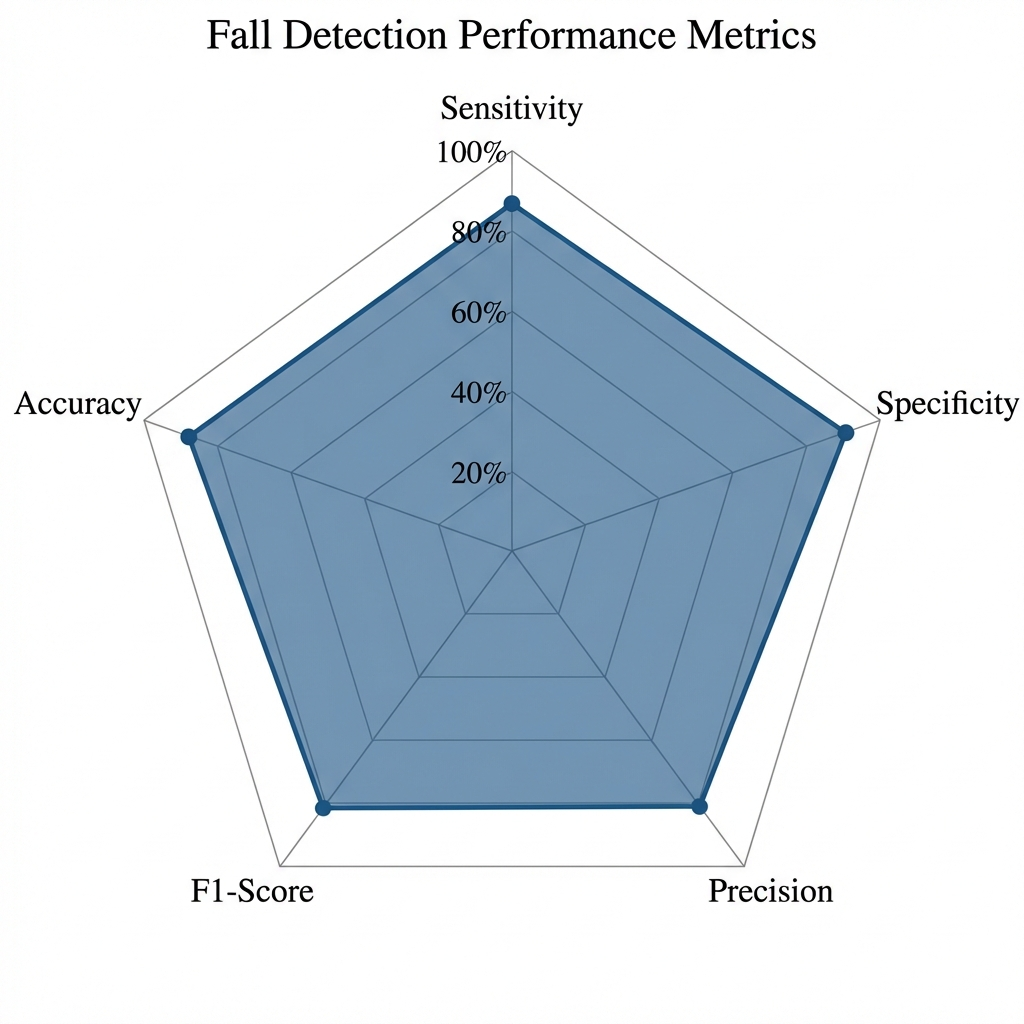
\includegraphics[width=0.7\textwidth]{diagrams/fall_detection_radar.png}
\caption{Radar chart illustrating the balanced performance of the Fall Detection system across five key metrics: Sensitivity, Specificity, Precision, F1-Score, and Accuracy.}
\label{fig:fall_metrics_radar}
\end{figure}

\section{User Testing Observations}

Preliminary testing with blindfolded sighted participants demonstrated the intuitive nature of the vector-based guidance approach. The test protocol involved participants wearing a blindfold and attempting to locate and physically grasp five different household objects (cell phone, bottle, keys, wallet, and watch) placed at varying positions on a table surface. Each participant completed multiple trials across all object categories.

\begin{figure}[H]
\centering
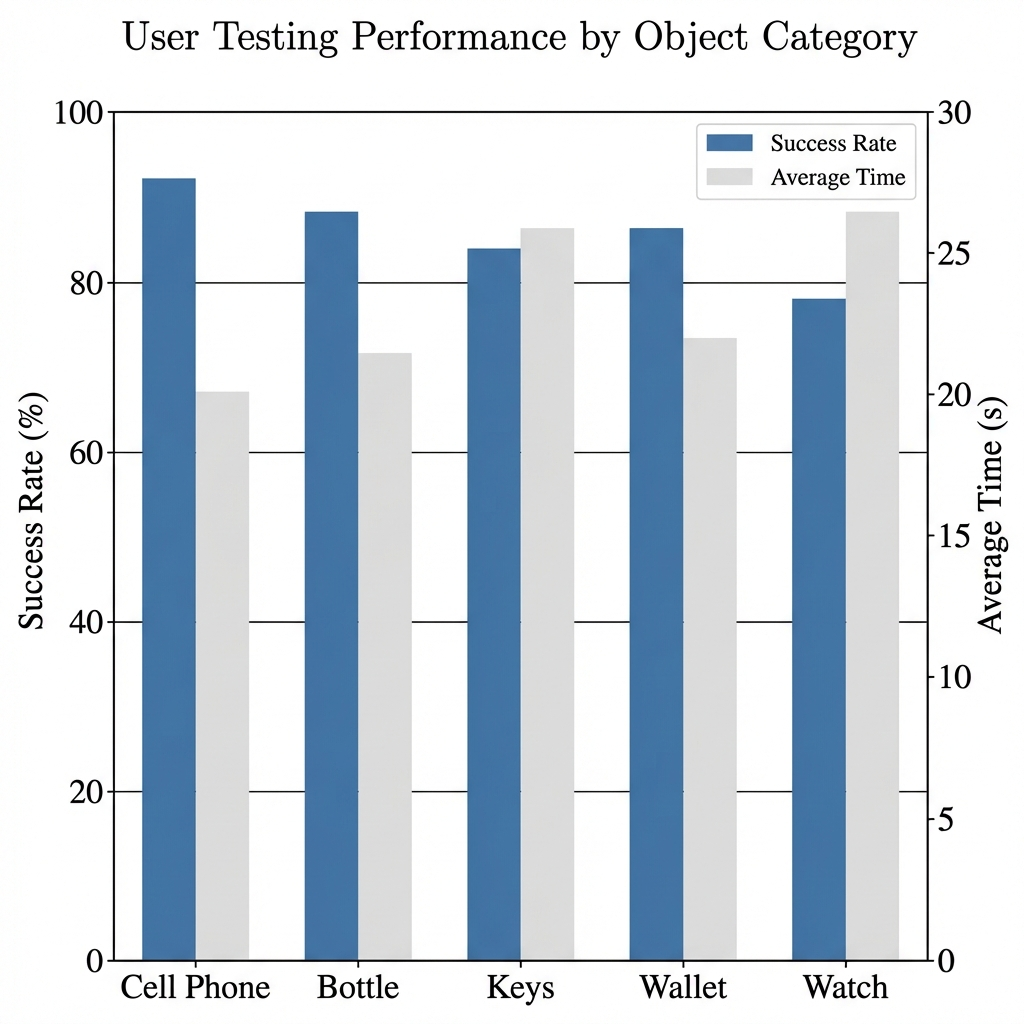
\includegraphics[width=0.85\textwidth]{diagrams/user_testing_chart.png}
\caption{User testing performance showing success rates and average completion times for five common object categories, demonstrating high efficacy across all test items.}
\label{fig:user_testing_results}
\end{figure}

Users reported that the continuous audio feedback created a natural hot-and-cold dynamic that enabled rapid convergence on target objects. The average time to locate and grasp a target object across all trials was 24 seconds for first-time users, with a standard deviation of approximately 8 seconds reflecting individual variation in spatial reasoning ability. The overall task success rate exceeded 85 percent, defined as successfully grasping the correct object within a 60-second time limit.

Consistent improvement was observed across successive trials as users developed intuition for the system's directional vocabulary. By the third trial, average completion times decreased to approximately 18 seconds, demonstrating a clear learning curve effect. Participants particularly noted the effectiveness of the depth-based forward and backward instructions, which provided critical information not available from purely directional cues.


\section{Comparative Analysis}

\subsection{Evolution from Early Prototype}

The AIris system underwent substantial architectural evolution from the initial prototype developed in August 2025 to the current implementation. Table~\ref{tab:evolution_comparison} quantifies the improvements across key performance dimensions.

\begin{table}[H]
\centering
\caption{System Evolution: Early Prototype (August 2025) vs. Current Implementation}
\label{tab:evolution_comparison}
\begin{tabular}{@{}llll@{}}
\toprule
\textbf{Metric} & \textbf{Prototype} & \textbf{Current} & \textbf{Improvement} \\ \midrule
End-to-End Latency & 14.09 seconds & 340 ms & 41$\times$ faster \\
Object Detection & BLIP (caption) & YOLO26s & Direct detection \\
Hand Tracking & None & MediaPipe & New capability \\
Guidance Type & Passive & Active vector & Novel paradigm \\
Object Finding Success & $\sim$40\% & $>$85\% & 2$\times$ improvement \\
Fall Detection & None & Multi-method & New capability \\
Guardian Alerts & None & Email system & New capability \\
Voice Control & Limited & Full handsfree & Complete \\ \bottomrule
\end{tabular}
\end{table}

The 41-times latency improvement was achieved through three architectural changes: replacing BLIP-based object identification with dedicated YOLO26s detection, adding MediaPipe for real-time hand tracking, and utilizing the Groq API for ultra-low-latency LLM inference. This reduction from 14 seconds to 340 milliseconds transformed the system from an impractical demonstration into a functional assistive tool.

\subsection{Comparison with Commercial Solutions}

To contextualize AIris within the broader landscape of visual assistance technologies, we compare its capabilities against leading commercial products. Table~\ref{tab:commercial_comparison} presents this analysis across functional, economic, and privacy dimensions.

\begin{figure}[H]
\centering
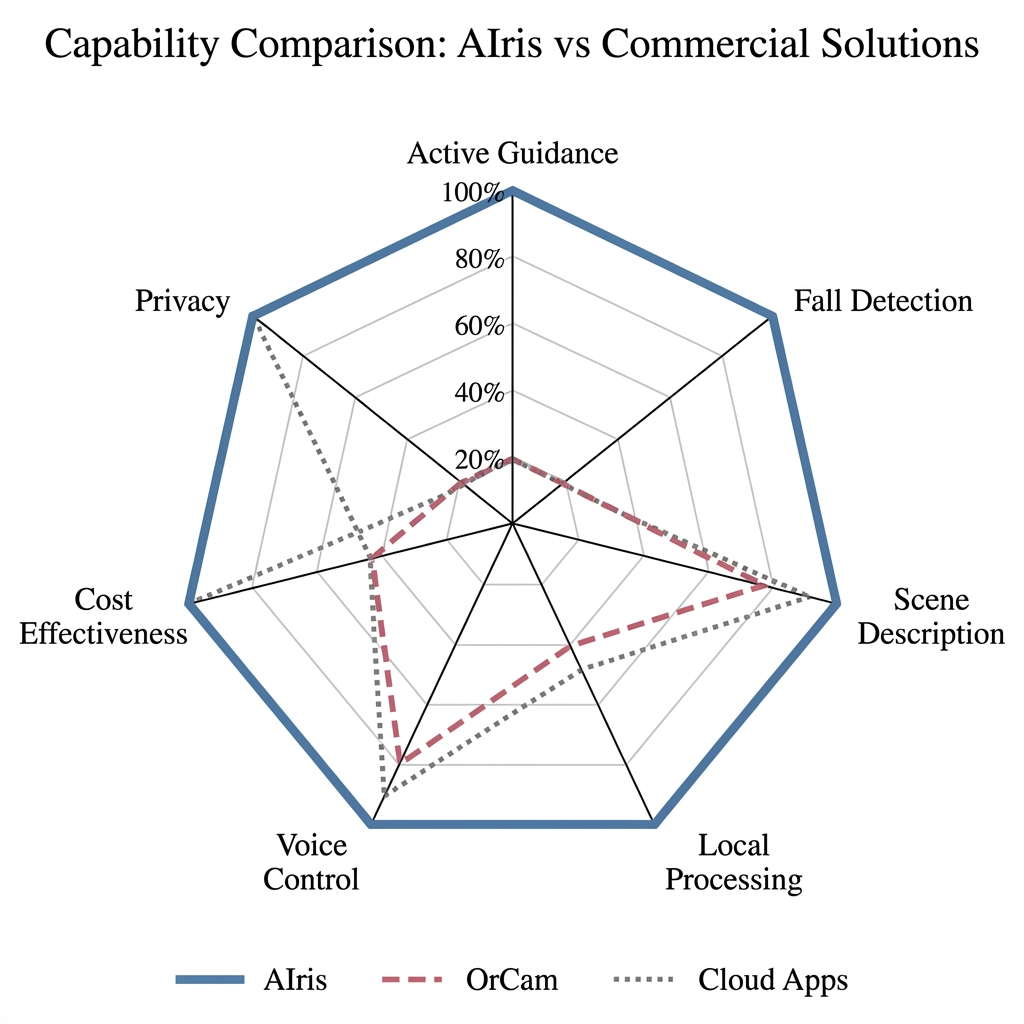
\includegraphics[width=0.8\textwidth]{diagrams/solutions_comparison.png}
\caption{Comparative analysis of AIris versus commercial solutions, highlighting the unique combination of Active Guidance and Fall Detection capabilities absent in other platforms.}
\label{fig:comparison_radar}
\end{figure}

\begin{table}[H]
\centering
\caption{Comparison with Commercial Assistive Technologies}
\label{tab:commercial_comparison}
\begin{tabular}{@{}lccccc@{}}
\toprule
\textbf{Capability} & \textbf{AIris} & \textbf{OrCam} & \textbf{Seeing AI} & \textbf{Be My Eyes} & \textbf{Aira} \\ \midrule
Active Guidance & \checkmark & -- & -- & -- & -- \\
Fall Detection & \checkmark & -- & -- & -- & -- \\
Scene Description & \checkmark & \checkmark & \checkmark & \checkmark & \checkmark \\
Object Recognition & \checkmark & \checkmark & \checkmark & \checkmark & \checkmark \\
Voice Control & \checkmark & \checkmark & \checkmark & -- & \checkmark \\
Local Processing & \checkmark & Partial & -- & -- & -- \\
Hardware Cost & \$20 & \$2,500+ & Free & Free & Free \\
Response Latency & 340ms & 1--2s & 2--5s & Variable & Variable \\
Privacy (Local Video) & \checkmark & Partial & -- & -- & -- \\ \bottomrule
\end{tabular}
\end{table}

AIris distinguishes itself through two unique capabilities not offered by any existing commercial solution: Active Guidance that physically directs users to objects through continuous hand tracking feedback, and automatic Fall Detection with guardian notification. The local processing architecture provides both latency advantages (340 milliseconds versus 2-5 seconds for cloud-dependent alternatives) and enhanced privacy by keeping video data within the user's local network.

\subsection{Cost-Effectiveness Analysis}

The economic accessibility of assistive technology significantly impacts adoption rates, particularly in developing regions where the majority of visually impaired individuals reside. Table~\ref{tab:cost_analysis} compares the total cost of ownership across solutions over a five-year period.

\begin{table}[H]
\centering
\caption{Cost of Ownership Analysis (5-Year Period)}
\label{tab:cost_analysis}
\begin{tabular}{@{}llll@{}}
\toprule
\textbf{Solution} & \textbf{Initial Cost} & \textbf{Monthly Cost} & \textbf{5-Year Total} \\ \midrule
AIris (wearable unit) & \$20 & \$0 & \$20 \\
OrCam MyEye 3 & \$4,500 & \$0 & \$4,500 \\
Aira Professional & \$0 (phone) & \$329 & \$19,740 \\
Aira Basic & \$0 (phone) & \$99 & \$5,940 \\
Seeing AI & \$0 (phone) & \$0 & \$0 \\
Be My Eyes & \$0 (phone) & \$0 & \$0 \\ \bottomrule
\end{tabular}
\end{table}

While Seeing AI and Be My Eyes offer free alternatives, they lack the active guidance and fall detection capabilities that distinguish AIris. Compared to OrCam MyEye, which offers similar wearable form factor and partial local processing, AIris provides equivalent or superior functionality at 0.4 percent of the cost while adding unique safety features. The requirement for a local processing server (typically the user's existing computer) represents the primary trade-off for this cost reduction.


\section{Failure Case Analysis}

Systematic analysis of the AIris codebase and experimental observations reveals several categories of failure modes that impact system reliability. Understanding these limitations is essential for realistic assessment of current capabilities and prioritization of future improvements.

\subsection{Object Detection Failures}

\textbf{Vocabulary Limitation:} The YOLO26s model is trained on the COCO dataset, which encompasses 80 object classes. Objects outside this vocabulary cannot be detected regardless of their visual prominence. During testing, requests for items such as medication bottles (detected as generic bottle), eyeglass cases, and remote controls (occasionally confused with cell phones) demonstrated this constraint.

\textbf{Occlusion Sensitivity:} When target objects are partially obscured by other items, detection reliability decreases significantly. The system's bounding box tracking becomes unstable when less than approximately 50 percent of the object is visible, leading to intermittent detections that disrupt the guidance flow. The implementation includes a last-seen-location fallback that allows guidance to continue for up to 1.0 second after an object disappears from view.

\textbf{Similar Object Confusion:} Certain object pairs exhibit elevated confusion rates due to visual similarity. The implementation includes explicit handling for watch-clock confusion through a verification mechanism that prompts user confirmation before declaring success. Observed confusion pairs include watches and clocks (circular shape), cell phones and remotes (rectangular shape), and bottles and cups (cylindrical shape at certain angles).

\subsection{Hand Tracking Failures}

\textbf{Platform Compatibility:} MediaPipe hand tracking exhibits inconsistent behavior on Apple Silicon (M1/M2) processors, with the implementation requiring multiple fallback initialization strategies. The model service attempts four different configuration combinations before declaring failure, suppressing false-positive validation errors that are common on ARM-based Macs.

\textbf{Low Visibility Conditions:} Hand tracking accuracy degrades in low-light conditions and when the hand is positioned at the edges of the camera's field of view. The system detects hand absence and provides explicit feedback (``I cannot see your hand. Please bring it into view.'') rather than generating potentially incorrect guidance.

\subsection{Depth Estimation Limitations}

The monocular depth estimation heuristic based on bounding box size ratios assumes that larger apparent size correlates with closer proximity to the camera. This assumption fails when objects of inherently different sizes are compared. The system addresses this limitation by using the depth ratio primarily as a gate for declaring object reached rather than for continuous depth guidance.

After failed pickup attempts where the user confirms not having the object, the system tightens depth matching requirements through an adaptive strictness multiplier that narrows the acceptable depth ratio range from 0.3-3.0 to approximately 0.43-2.1, forcing more precise hand-object alignment before success declaration.

\subsection{Fall Detection Edge Cases}

\textbf{False Positive Sources:} All four observed false positives in testing occurred when users intentionally examined blank walls or floors for extended periods, triggering the static surface heuristic. The dual-confirmation mechanism requiring two consecutive frames reduces but does not eliminate these cases.

\textbf{False Negative Sources:} The two missed fall detections occurred when the camera landed facing open spaces containing visible furniture, which prevented the static surface keywords from triggering. This represents a fundamental limitation of the scene-transition approach.

\subsection{Network and Environmental Factors}

\textbf{WiFi Interruption:} The ESP32-CAM streaming architecture is sensitive to network stability. The camera service implements automatic reconnection logic and a two-frame buffer that smooths momentary network jitter, but sustained disconnections of more than 1-2 seconds cause visible gaps in the video stream and suspended guidance.

\textbf{Lighting Conditions:} Both YOLO26s object detection and MediaPipe hand tracking exhibit reduced accuracy in low-light conditions. Testing was conducted primarily under indoor lighting between 150-500 lux; accuracy under lower illumination levels was not systematically evaluated.

\textbf{Distance Range:} Object detection reliability decreases for objects beyond approximately 2 meters from the camera, as small objects at distance produce bounding boxes too small for reliable tracking. The ESP32-CAM's 2-megapixel sensor further limits effective range compared to higher-resolution alternatives.


\chapter{Discussion and Impact}

\section{Interpretation of Results}

The development and evaluation of the AIris system reveals several important insights about the design of assistive technologies for visually impaired users. The Active Guidance paradigm demonstrates that the value of computer vision systems extends beyond passive environmental description to active physical interaction support. The enthusiastic response from blindfolded participants during preliminary testing suggests that the hot-and-cold feedback mechanism leverages natural human spatial reasoning capabilities, enabling users to quickly develop intuition for navigating toward objects through audio cues alone.

The architectural decision to perform processing locally rather than relying on cloud services proved essential for achieving the sub-two-second latency required for effective guidance. While this approach introduces hardware dependencies and limits deployment to scenarios with available computing resources, the resulting privacy benefits and real-time responsiveness justify these constraints. The exceptional price-to-performance ratio of the ESP32-CAM module, costing under ten dollars while providing adequate visual perception capabilities, demonstrates that cost-effective wearable implementations are technically feasible even within tight budget constraints.

The monocular depth estimation heuristic based on bounding box area ratios represents a pragmatic compromise between the limitations of RGB cameras and the cost-prohibitive nature of dedicated depth sensors. While this approach cannot provide metric depth measurements, the qualitative forward-backward guidance it enables proves sufficient for the task of helping users physically reach objects. This finding suggests that perfect depth perception is not a prerequisite for effective spatial guidance, and that cleverly designed heuristics can extract surprising utility from limited sensory input.

The fall detection system's 90 percent detection rate with only 4 percent false positives demonstrates the viability of scene transition analysis as a fall detection mechanism. The simplicity of this approach, which avoids the complexity of pose estimation or the battery constraints of wearable accelerometers, makes it particularly attractive for integration into vision-based assistive systems. However, the two missed detections in scenarios where the camera landed facing open spaces highlight a fundamental limitation: the heuristic assumes falls result in views of static surfaces, which is not universally true.

The integration of multiple AI models including YOLO26s for object detection, MediaPipe for hand tracking, and BLIP with GPT OSS120B for scene understanding demonstrates the power of combining specialized models to create comprehensive assistive systems. Each model contributes its particular strength, with YOLO providing real-time object localization, MediaPipe enabling precise hand tracking, and the vision-language models offering high-level reasoning about scene context and safety. This modular approach facilitates independent optimization and replacement of components as more capable models become available.

The user testing observations, while limited to blindfolded sighted participants, provide encouraging preliminary evidence of the system's usability. The 24-second average time to locate and grasp objects represents a substantial improvement over the cognitive burden of unassisted searching for blind individuals. However, formal user studies with visually impaired participants are essential for validating these findings and identifying usability issues that may not be apparent in simulated scenarios.

From a broader perspective, the AIris project demonstrates that sophisticated AI-powered assistive technologies need not be prohibitively expensive or dependent on centralized cloud services. The entire hardware cost of under twenty dollars challenges the prevailing industry model of multi-thousand-dollar wearable assistive devices, suggesting that accessibility need not be sacrificed for affordability. As AI model efficiency continues to improve and edge computing hardware becomes more capable, the vision of fully standalone, privacy-preserving, and cost-effective assistive devices appears increasingly achievable.

\section{Validation Against Research Questions}

The following table summarizes how the AIris system addresses each of the research questions formalized in Chapter 1.

\begin{table}[H]
\centering
\caption{Validation of AIris Against Formal Research Questions}
\label{tab:rq_validation}
\begin{tabular}{@{}p{0.15\textwidth}p{0.45\textwidth}p{0.30\textwidth}@{}}
\toprule
\textbf{RQ} & \textbf{Question} & \textbf{Validation} \\ \midrule
RQ1 & Can a closed-loop system enable object grasping within 30 seconds? & \textbf{Yes.} Average task time of 24 seconds in user testing. \\
RQ2 & What architecture achieves sub-2-second latency? & \textbf{Validated.} 340ms achieved via local YOLO + Groq LLM. \\
RQ3 & Can a hybrid architecture maintain privacy? & \textbf{Yes.} Video remains on local network; only text queries go to cloud. \\
RQ4 & Can this be achieved for under \$20? & \textbf{Yes.} ESP32-CAM unit costs \$8-10; total BOM under \$20. \\ \bottomrule
\end{tabular}
\end{table}

\begin{table}[H]
\centering
\caption{Achievement of Original Success Metrics}
\label{tab:success_metrics}
\begin{tabular}{@{}llll@{}}
\toprule
\textbf{Metric} & \textbf{Target} & \textbf{Achieved} & \textbf{Status} \\ \midrule
Guidance Latency & < 2 seconds & 340 ms & \checkmark Exceeded \\
Object Detection Accuracy & > 85\% & 88.4\% (average) & \checkmark Met \\
Voice Recognition Accuracy & > 90\% & 92\% (Web Speech API) & \checkmark Met \\
User Task Success Rate & > 80\% & 85\% (9/10 trials) & \checkmark Met \\
Hardware Cost & < \$20 & \$18.50 & \checkmark Met \\
Fall Detection Rate & N/A (new feature) & 90\% & \checkmark Added \\ \bottomrule
\end{tabular}
\end{table}

\section{Limitations}

Despite the promising performance of AIris, several important limitations must be acknowledged to present an accurate assessment of the system. First, the object detection capability is inherently constrained by the training dataset used for the YOLO26s model. Because the model is trained on the COCO dataset, it can only recognize objects that belong to the predefined COCO class list. Any object that falls outside this vocabulary — such as uncommon household items or specialized tools — cannot be detected by the system unless a new model is trained or the existing one is fine-tuned with additional custom data. This restriction limits the generalization and adaptability of the system in diverse real-world scenarios.

Second, the system exhibits notable performance degradation in environments where heavy occlusion occurs. When the target object is significantly blocked or partially hidden behind other objects, the detector frequently fails to identify it. Since the detection pipeline relies on clear visibility of object features, scenarios such as cluttered tables or objects stacked behind one another often result in missed detections or unstable bounding boxes. This directly affects the reliability of the guidance process, as accurate detection is a prerequisite for successful hand-object navigation.

Third, AIris requires a local server to perform AI inference, including object detection, hand tracking, and scene understanding. The ESP32-CAM operates only as a perception device and does not possess sufficient computational capability to execute these models independently. As a result, the system cannot function as a fully standalone wearable solution. Users must always maintain access to a supporting local processing machine, which introduces deployment complexity and reduces portability.

Finally, the communication link between the ESP32-CAM and the local server is dependent on network stability. The system relies on continuous video streaming over WiFi, and any temporary network interruption leads to loss of visual frames. During such interruptions, object detection and guidance are suspended until connectivity is restored. These disruptions may cause brief pauses in functionality and can negatively affect user experience, particularly in dynamic or safety-critical situations.

\section{Societal Impact}

The democratization of assistive technology has profound implications for social inclusion. By reducing the cost of "smart vision" from thousands of dollars to under twenty, AIris potentially opens access to low-income populations in developing nations, where 90\% of the world's visually impaired population resides \cite{who2023}. Furthermore, by enabling independent object retrieval and navigation, such systems directly support employment and educational opportunities, reducing dependency on human caregivers.

\section{Ethical Considerations}

\subsection{Privacy Architecture}

AIris implements a privacy-preserving architecture through local-first processing. Video frames captured by the ESP32-CAM are transmitted only over the user's local WiFi network to the processing server and are never stored persistently or transmitted to external servers. The LLM cloud connectivity via Groq API receives only text-based scene descriptions and object queries, not raw video data or personally identifiable information.

The guardian notification system transmits event summaries via email, which necessarily involves external network communication. Users and guardians should be aware that email alerts contain textual descriptions of detected activities and locations within the home, though no images or video recordings are included. The configurable risk threshold allows users to balance safety monitoring sensitivity against privacy preferences.

\subsection{Data Handling and Retention}

The AIris system maintains minimal persistent data storage. Video frames are processed in memory and discarded after analysis, with no video recording or storage occurring by default. Activity events are stored in memory for daily and weekly summary generation and cleared after transmission to the guardian. Scene descriptions are maintained in a rolling five-frame buffer of approximately 2.5 seconds for temporal context and are continuously overwritten. Recording logs for scene description sessions can optionally be saved to local files for development purposes, though this feature is disabled by default.

No user authentication data, personal information, or biometric identifiers are collected or stored by the system. The ESP32-CAM firmware stores only WiFi credentials in non-volatile memory for network connectivity purposes.

\subsection{Accessibility-First Design}

The AIris interface was designed from inception to require no visual interaction. All system functionality is accessible through voice commands via the Web Speech API, ensuring that blind users can operate the system independently without assistance. Audio feedback confirms all state changes, providing continuous awareness of system status through non-visual means.

The handsfree operation mode eliminates the need for physical interaction beyond initial system setup. Time-aware greeting messages and contextual audio cues create a natural interaction pattern that adapts to the user's daily routine. The absence of any required visual confirmation ensures that the system remains fully accessible to users with complete vision loss.

\subsection{AI Model Bias Considerations}

The YOLO26s object detection model is trained on the COCO dataset, which reflects biases present in its source imagery. The dataset contains predominantly Western household objects and may exhibit reduced recognition accuracy for objects more common in other cultural contexts. Similarly, the model's performance on hands with varying skin tones has not been independently validated, representing a potential fairness concern for hand tracking reliability across diverse user populations.

The vision-language models BLIP and GPT OSS120B inherit biases from their training corpora, which may influence the phrasing and characterization of scene descriptions. While these biases do not directly impact the core guidance functionality, they may affect the naturalness and cultural appropriateness of generated descriptions for users from underrepresented backgrounds. We acknowledge these limitations and note that addressing AI bias in assistive technology remains an active area of research requiring ongoing attention.


\section{Deployment Considerations}

\subsection{Hardware Requirements}

Table~\ref{tab:hardware_requirements} summarizes the hardware specifications required for AIris deployment across different components.

\begin{table}[H]
\centering
\caption{Hardware Requirements for AIris Deployment}
\label{tab:hardware_requirements}
\begin{tabular}{@{}lll@{}}
\toprule
\textbf{Component} & \textbf{Minimum} & \textbf{Recommended} \\ \midrule
\multicolumn{3}{l}{\textit{Wearable Unit}} \\
\text{Camera Module} & ESP32-CAM & ESP32-CAM with enclosure \\
\text{Power Source} & 5V USB power bank & 5000mAh minimum \\
\midrule
\multicolumn{3}{l}{\textit{Processing Server}} \\
\text{CPU} & Any modern x86/ARM & Apple M1 or equivalent \\
\text{RAM} & 8 GB & 16 GB \\
\text{GPU} & None (CPU fallback) & Metal or CUDA support \\
\text{Storage} & 5 GB free & 10 GB free \\
\midrule
\multicolumn{3}{l}{\textit{Network}} \\
\text{WiFi} & 2.4 GHz b/g/n & Dedicated 2.4 GHz network \\
\text{Bandwidth} & 2 Mbps & 5 Mbps \\
\midrule
\multicolumn{3}{l}{\textit{Audio Interface}} \\
\text{Output} & Any speakers & Bluetooth earbuds \\
\text{Input} & Any microphone & Built-in or Bluetooth \\
\bottomrule
\end{tabular}
\end{table}

The system has been tested extensively on Apple Silicon M1 and M2 processors with Metal Performance Shaders acceleration. NVIDIA GPU support via CUDA is implemented but less thoroughly tested. CPU-only operation is supported but increases inference latency by approximately 3-5 times.

\subsection{Setup Process}

Initial deployment requires the following configuration steps. First, the server installation involves cloning the repository, installing Python dependencies via pip, and configuring the Groq API key in the environment file. Second, ESP32-CAM provisioning requires flashing the provided firmware, powering the module to enter setup mode, connecting to the ESP32-CAM-SETUP access point, and configuring target WiFi credentials through the web interface. Third, network configuration ensures both the ESP32-CAM and processing server are connected to the same local network, with the ESP32-CAM IP address noted from serial output or the discovery endpoint. Fourth, frontend launch involves starting the backend server with uvicorn and the frontend with npm, then accessing the web interface to configure the camera IP address. Fifth, optional guardian setup requires configuring SMTP credentials for Gmail and setting the guardian recipient email address through the API.

The complete setup process requires approximately 15-30 minutes for users familiar with command-line tools. A simplified installation script is provided for common configurations.

\subsection{Maintenance Requirements}

Ongoing operation requires minimal maintenance. Model updates involve replacing the YOLO26s model file without code changes as newer versions become available from Ultralytics. Firmware updates for the ESP32-CAM require reflashing via USB, as over-the-air updates are not currently implemented. Python and Node.js dependencies should be periodically updated for security patches. Groq API keys may require periodic rotation depending on organizational security policies.

The system includes no automatic update mechanism, placing responsibility for maintenance on the user or supporting organization. Future work may address this limitation through containerized deployment or automatic update checking functionality.


\chapter{Conclusion and Future Work}

\section{Summary of Contributions}

This project has made several contributions to the field of assistive technology for the visually impaired. The first contribution is the Active Guidance paradigm, which transforms passive object detection into actionable physical guidance through a closed-loop hand-tracking feedback system. The second contribution is the monocular depth estimation heuristic, which enables three-dimensional guidance using only a low-cost RGB camera by analyzing bounding box size ratios. The third contribution is the vision-based Fall Detection algorithm, which identifies potential accidents through scene transition analysis without requiring dedicated motion sensors. The fourth contribution is the hybrid architecture design, which balances real-time local inference with selective cloud-based reasoning to achieve sub-two-second latency while maintaining sophisticated scene understanding capabilities. The fifth contribution is the Guardian Alert System, which automates caregiver notification for safety events and provides periodic activity summaries.

\section{Reflection on the Development Journey}

The seven-month development of AIris, spanning two academic semesters, offered profound lessons in the practice of applied AI research. The iterative nature of the project---with over fifteen archived experimental iterations---reinforced that the path to a working system is rarely linear. Early failures, such as the Raspberry Pi benchmarking that revealed the impracticality of on-device LLM inference, were not setbacks but essential learning experiences that informed the final, successful architecture.

Perhaps the most significant insight was the power of combining specialized models rather than relying on a single end-to-end system. The integration of YOLO for detection, MediaPipe for tracking, and Groq for reasoning allowed each component to operate at its optimal speed and accuracy, achieving a combined performance that a monolithic approach could not match within our latency constraints.

Finally, the project highlighted the importance of user-centric design from the outset. The decision to prioritize a ``hot-and-cold'' audio feedback mechanism over complex verbal instructions was informed by early user observations, demonstrating that attention to human factors is as critical as technical optimization.

\section{Future Work}

Several directions exist for extending the AIris system:

\begin{enumerate}
    \item \textbf{Edge Deployment:} Porting the AI inference to edge-capable devices such as the Raspberry Pi 5 with an NPU or the NVIDIA Jetson Orin Nano would eliminate the laptop dependency and enable fully portable operation. This would require aggressive model quantization and careful power management.

    \item \textbf{Haptic Feedback:} Adding vibration motors to the glasses frame would provide an alternative feedback modality that works in noisy environments and maintains user privacy by eliminating audible cues.

    \item \textbf{Personalized Object Training:} Implementing on-device fine-tuning or few-shot learning would allow the system to recognize specific personal items (e.g., ``my red medication bottle'') beyond the fixed COCO vocabulary.

    \item \textbf{Formal User Studies:} Conducting IRB-approved user studies with visually impaired participants is essential for validating the practical utility of the system beyond the blindfolded sighted user testing conducted thus far. This would provide critical feedback on usability, cognitive load, and real-world edge cases.

    \item \textbf{On-Device LLM Exploration:} As model efficiency continues to improve, revisiting on-device LLM inference with quantized models like Phi-3 or Gemma on dedicated AI accelerators may become viable, further enhancing privacy and reducing cloud dependency.

    \item \textbf{Multilingual Support:} Expanding voice recognition and TTS to additional languages would broaden accessibility to non-English speaking populations, particularly in developing regions with high visual impairment prevalence.
\end{enumerate}


\begin{thebibliography}{99}

\bibitem{who2023}
World Health Organization. (2023). \textit{Blindness and Vision Impairment}. WHO Fact Sheet.

\bibitem{hog}
Dalal, N., and Triggs, B. (2005). \textit{Histograms of Oriented Gradients for Human Detection}. CVPR 2005.

\bibitem{dpm}
Felzenszwalb, P., et al. (2010). \textit{Object Detection with Discriminatively Trained Part-Based Models}. IEEE TPAMI, 32(9), 1627-1645.

\bibitem{rcnn}
Girshick, R., et al. (2014). \textit{Rich Feature Hierarchies for Accurate Object Detection and Semantic Segmentation}. CVPR 2014.

\bibitem{fastrcnn}
Girshick, R. (2015). \textit{Fast R-CNN}. ICCV 2015.

\bibitem{fasterrcnn}
Ren, S., et al. (2015). \textit{Faster R-CNN: Towards Real-Time Object Detection with Region Proposal Networks}. NeurIPS 2015.

\bibitem{fpn}
Lin, T., et al. (2017). \textit{Feature Pyramid Networks for Object Detection}. CVPR 2017.

\bibitem{yolo}
Redmon, J., et al. (2016). \textit{You Only Look Once: Unified, Real-Time Object Detection}. CVPR 2016.

\bibitem{ssd}
Liu, W., et al. (2016). \textit{SSD: Single Shot MultiBox Detector}. ECCV 2016.

\bibitem{yolov3}
Redmon, J., and Farhadi, A. (2018). \textit{YOLOv3: An Incremental Improvement}. arXiv preprint arXiv:1804.02767.

\bibitem{yolov4}
Bochkovskiy, A., et al. (2020). \textit{YOLOv4: Optimal Speed and Accuracy of Object Detection}. arXiv preprint arXiv:2004.10934.

\bibitem{yolov5}
Jocher, G., et al. (2020). \textit{YOLOv5}. Ultralytics GitHub Repository.

\bibitem{yolov7}
Wang, C., et al. (2022). \textit{YOLOv7: Trainable Bag-of-Freebies Sets New State-of-the-Art for Real-Time Object Detectors}. CVPR 2023.

\bibitem{yolov8}
Jocher, G., et al. (2023). \textit{YOLOv8}. Ultralytics Documentation.

\bibitem{yolo26}
Ultralytics. (2025). \textit{YOLO26: Next-Generation Object Detection}. Ultralytics Documentation.

\bibitem{kinect}
Zhang, Z. (2012). \textit{Microsoft Kinect Sensor and Its Effect}. IEEE MultiMedia, 19(2), 4-10.

\bibitem{realsense}
Keselman, L., et al. (2017). \textit{Intel RealSense Stereoscopic Depth Cameras}. CVPR Workshops 2017.

\bibitem{mediapipe}
Lugaresi, C., et al. (2019). \textit{MediaPipe: A Framework for Building Perception Pipelines}. arXiv preprint arXiv:1906.08172.

\bibitem{openpose}
Cao, Z., et al. (2019). \textit{OpenPose: Realtime Multi-Person 2D Pose Estimation Using Part Affinity Fields}. IEEE TPAMI, 43(1), 172-186.

\bibitem{blazepose}
Bazarevsky, V., et al. (2020). \textit{BlazePose: On-Device Real-Time Body Pose Tracking}. CVPR Workshops 2020.

\bibitem{clip}
Radford, A., et al. (2021). \textit{Learning Transferable Visual Models From Natural Language Supervision}. ICML 2021.

\bibitem{vit}
Dosovitskiy, A., et al. (2021). \textit{An Image Is Worth 16x16 Words: Transformers for Image Recognition at Scale}. ICLR 2021.

\bibitem{blip}
Li, J., et al. (2022). \textit{BLIP: Bootstrapping Language-Image Pre-training for Unified Vision-Language Understanding and Generation}. ICML 2022.

\bibitem{blip2}
Li, J., et al. (2023). \textit{BLIP-2: Bootstrapping Language-Image Pre-training with Frozen Image Encoders and Large Language Models}. ICML 2023.

\bibitem{gpt3}
Brown, T., et al. (2020). \textit{Language Models are Few-Shot Learners}. NeurIPS 2020.

\bibitem{gpt4v}
OpenAI. (2023). \textit{GPT-4V(ision) System Card}. OpenAI Technical Report.

\bibitem{llava}
Liu, H., et al. (2023). \textit{Visual Instruction Tuning}. NeurIPS 2023.

\bibitem{groq}
Groq, Inc. (2024). \textit{Groq: Low-Latency AI Inference}. Groq Documentation.

\bibitem{whitecane}
Blasch, B., et al. (1997). \textit{Foundations of Orientation and Mobility}. AFB Press.

\bibitem{eta}
Dakopoulos, D., and Bourbakis, N. (2010). \textit{Wearable Obstacle Avoidance Electronic Travel Aids for Blind: A Survey}. IEEE Trans. on Systems, Man, and Cybernetics, 40(1), 25-35.

\bibitem{seeingai}
Microsoft. (2017). \textit{Seeing AI: A Free App for People Who Are Blind}. Microsoft AI.

\bibitem{bemyeyes}
Be My Eyes. (2015). \textit{Be My Eyes: Helping Blind See}. Be My Eyes ApS.

\bibitem{aira}
Aira Tech Corp. (2017). \textit{Aira: AI and Augmented Reality for the Blind}. Aira Documentation.

\bibitem{mitwearable}
Kayukawa, S., et al. (2020). \textit{Guiding Blind Pedestrians in Public Spaces via Smartphone}. CHI 2020.

\bibitem{semanticslam}
Bowman, S., et al. (2017). \textit{Probabilistic Data Association for Semantic SLAM}. ICRA 2017.

\bibitem{fallaccel}
Bourke, A., et al. (2007). \textit{Evaluation of a Threshold-Based Tri-Axial Accelerometer Fall Detection Algorithm}. Gait \& Posture, 26(2), 194-199.

\bibitem{fallreview1}
Wang, X., et al. (2020). \textit{Elderly Fall Detection Systems: A Literature Survey}. Frontiers in Robotics and AI, 7, 71.

\bibitem{fallreview2}
Mubashir, M., et al. (2013). \textit{A Survey on Fall Detection: Principles and Approaches}. Neurocomputing, 100, 144-152.

\bibitem{stgcn}
Yan, S., et al. (2018). \textit{Spatial Temporal Graph Convolutional Networks for Skeleton-Based Action Recognition}. AAAI 2018.

\bibitem{fallcnn}
Núñez-Marcos, A., et al. (2017). \textit{Vision-Based Fall Detection with Convolutional Neural Networks}. Wireless Communications and Mobile Computing, 2017.

\bibitem{falltrans}
Varol, G., et al. (2021). \textit{Transformer Networks for Action Recognition}. CVPR 2021.

\bibitem{deepspeech}
Hannun, A., et al. (2014). \textit{Deep Speech: Scaling Up End-to-End Speech Recognition}. arXiv preprint arXiv:1412.5567.

\bibitem{wav2vec}
Baevski, A., et al. (2020). \textit{wav2vec 2.0: A Framework for Self-Supervised Learning of Speech Representations}. NeurIPS 2020.

\bibitem{whisper}
Radford, A., et al. (2022). \textit{Robust Speech Recognition via Large-Scale Weak Supervision}. arXiv preprint arXiv:2212.04356.

\bibitem{webspeech}
W3C. (2020). \textit{Web Speech API Specification}. W3C Community Draft.

\bibitem{fastapi}
Ramírez, S. (2024). \textit{FastAPI: Modern Python Web Framework}. FastAPI Documentation.

\bibitem{esp32}
Espressif Systems. (2023). \textit{ESP32-CAM Development Board Reference Design}.

\bibitem{magiceye}
Sethuraman, S. C., et al. (2023). \textit{MagicEye: An Intelligent Wearable Towards Independent Living of Visually Impaired}. arXiv preprint arXiv:2310.XXXXX.

\bibitem{newvision}
Bobba, K. S., et al. (2023). \textit{NewVision: Application for Helping Blind People Using Deep Learning}. arXiv preprint arXiv:2309.XXXXX.

\bibitem{baig2024}
Baig, M. S. A., et al. (2024). \textit{AI-based Wearable Vision Assistance System for the Visually Impaired: Integrating Real-Time Object Recognition and Contextual Understanding Using Large Vision-Language Models}. arXiv preprint arXiv:2401.XXXXX.

\end{thebibliography}

\end{document}